% main file
\documentclass[12pt, twoside, a4paper, openright]{book}

%\newcommand{\euskaraz}{eu} % Comentar para castellano

% Nota Importante: En el caso de castellano, la codificación de los archivos
% deberá ser utf-8

% Codificación del archivo / fitxategiaren kudeaketa
\usepackage{ucs}
\usepackage[utf8x]{inputenc}
\usepackage[T1]{fontenc}


% ################################################################
% #######     SIZE OF THE PAGES                     ##############
% ################################################################
\usepackage[left=3.5cm, right=2.5cm, top=4.0cm, bottom=3.0cm]{geometry}
% \usepackage[left=1.5cm, right=2.5cm, top=2.0cm, bottom=2.0cm]{geometry}


% ################################################################
% #######     HEADERS                               ##############
% ################################################################
\usepackage{fancyhdr}           % Para cambiar las cabeceras de las pginas

\pagestyle{fancy}
\renewcommand{\chaptermark}[1]{ \markboth{#1}{} }
\renewcommand{\sectionmark}[1]{ \markright{#1}{} }

\fancyhf{}
\fancyhead[LE,RO]{\thepage}
\fancyhead[RE]{\textit{ \nouppercase{\leftmark}} }
\fancyhead[LO]{\textit{ \nouppercase{\rightmark}} }

\fancypagestyle{plain}{ %
  \fancyhf{} % remove everything
  \renewcommand{\headrulewidth}{0pt} % remove lines as well
  \renewcommand{\footrulewidth}{0pt}
}


	% Redefine plain page style
	\fancypagestyle{plain}{
		\fancyhf{}
		\renewcommand{\headrulewidth}{0pt}
		\fancyfoot[LE,RO]{\thepage}
	}

	% Define pagestyle
	\pagestyle{fancy}
	\fancyhf{}
	% \renewcommand{\chaptermark}[1]{\markboth{ \emph{#1}}{}}
	\fancyhead[LO]{}
	\fancyhead[RE]{\leftmark}
	\fancyfoot[LE,RO]{\thepage}

	% Code for creating empty pages
	% No headers on empty pages before new chapter
	% \makeatletter
	% \def\cleardoublepage{\clearpage\if@twoside \ifodd\c@page\else
		% \hbox{}
		% \thispagestyle{plain}
		% \newpage
		% \if@twocolumn\hbox{}\newpage\fi\fi\fi}
	% \makeatother \clearpage{\pagestyle{plain}\cleardoublepage}

	% Otra opción: considerar si funciona
	% this next section (till \makeatother) makes sure that blank pages
	%% are actually completely blank, cause they're not usually
	\makeatletter
	\def\cleardoublepage{\clearpage\if@twoside \ifodd\c@page\else
		\hbox{}
		\vspace*{\fill}
		\thispagestyle{empty}
		\newpage
		\if@twocolumn\hbox{}\newpage\fi\fi\fi}
	\makeatother


	% \pagestyle{fancy}				% use fancyhdr style
	% \setlength{\headheight}{13pt}

	% Limpiar estilo actual
	% \fancyhead{}
	% \fancyfoot{}
	% % or \fancyhf{}

	% \renewcommand{\headrulewidth}{0.4pt}    % Cabecera: subraya la cabecera (fijar en "0pt" si no se desea).
	% \renewcommand{\footrulewidth}{0pt}      % Pié: subraya el pie de página (fijar en "0pt" si no se desea).

	% There are seven letters you need to know before you can define your own header/footer:
	% E: Even page
	% O: Odd page
	% L: Left field
	% C: Center field
	% R: Right field
	% H: Header
	% F: Footer

% 	\fancyhead[CO,CE]{---Draft---}
% 	\fancyfoot[CO,CE]{Confidential}

% 	\fancyfoot[RO, LE] {\thepage}
% 	% or \fancyhf[FRO,FLE]...
% 
% 	\fancyhead[RE]{\nouppercase{\leftmark}}	% Cabecera: incluye información del nivel superior (Capítulo) % a la derecha (R) de las páginas pares (E), evitando escribir % todo en mayúsculas (que sería la opción por defecto).
% 	% or \fancyhf[HRE]...
% 
% 	\fancyhead[LO]{\nouppercase{\rightmark}}% Cabecera: incluyer información del nivel inferior (Sección) % a la izquierda (L) de las páginas impares (O), evitando escribir % todo en mayúsculas (que sería la opción por defecto).

	% \renewcommand{\chaptermark}[1]{%
		% \markboth{\small\slshape\chaptername{} \thechapter: #1}{}
		% }
	% \renewcommand{\sectionmark}[1]{%
		% \markright{\small\slshape\thesection : #1}
		% }

\renewcommand{\chaptermark}[1]{\markboth{#1}{}}
\renewcommand{\sectionmark}[1]{\markright{\thesection\ #1}}


%% which sections are numbered
\setcounter{secnumdepth}{2}

 
% ################################################################
% #######     Bibliografia                          ##############
% ################################################################
% \usepackage{natbib}
% \newcommand{\citenp}[2][ ]{\citeauthor{#2}#1 (\citeyear{#2})}
% \bibpunct{}{}{;}{a}{,}{,~}
% \newcommand{\myetal}{\emph{et~al.}}
% \bibliographystyle{plainnat4}
\bibliographystyle{apalike}


% To insert development comments (todos, corrections...)
\usepackage[textsize=scriptsize,textwidth=2cm]{todonotes}
% How to use: 
% - \todo{comentario/iruzkina} (insert into tex)
% - \todo[inline]{}

% ################################################################
% #######     FONT TYPES                            ##############
% ################################################################
% Charter
%\usepackage[bitstream-charter]{mathdesign}
% 	\renewcommand{\rmdefault}{mdbch} % charter
\DeclareSymbolFont{usualmathcal}{OMS}{cmsy}{m}{n}
\DeclareSymbolFontAlphabet{\mathcal}{usualmathcal}
%\usepackage{charter}
% \renewcommand{\rmdefault}{bch}
% \renewcommand{\bfdefault}{b}

% times erabili beharrean
\usepackage{mathptmx}
\usepackage[scaled=.90]{helvet}

% \renewcommand{\rmdefault}{ppl}
% \usepackage{mathpazo} % palatino
% \linespread{1.05}        % Palatino needs more leading
% \usepackage[bitstream-charter]{mathdesign}
% \usepackage{libertine}

%\usepackage[scaled]{berasans}

%\usepackage[scaled]{beramono}
% \renewcommand{\sfdefault}{fxbf}
	% libertine
% 		\renewcommand{\rmdefault}{fxlj} % Linux libertine 


% Sans serif


% ################################################################
% #######     GRAPHICS                              ##############
% ################################################################
\usepackage{graphicx}
\DeclareGraphicsExtensions{.png,.gif,.jpg,.pdf}
% \graphicspath{./irudiak/}
% \newcommand{\irudia}[3]{%
	% \begin{figure}[htb!]
	% \centering%
	% \includegraphics[width=#2]{#1}
	% \caption{#3}
	% \label{fig:#1}
	% \end{figure}
% }

\usepackage[figuresright]{rotating}

\newcommand{\fitx}[1]{\texttt{#1}}

%%%%%%%%%%%%%%%%%%%%%%%%%%%%%%%%%%%%%%%%%%%%%%%%%%%%%%%%%%%%%%%%
%%%%%%%%%%%  PARRAFOEN ESTILOA    %%%%%%%%%%%%%%%%%%%%%%%%%%%%
\frenchspacing
\widowpenalty=1000

% \titlespacing{\section}{1pc}{0ex plus .1ex minus .2ex}{1pc}
% \titlespacing{\section}{0pt}{*1}{*1}
\setlength{\parindent}{0cm} % anula indentacion de parrafos
\setlength{\parskip}{1.5ex plus 0.5ex minus 0.5ex}   % establece separacion entre parrafos a 8 puntos

\setlength\headheight{15pt}

\usepackage{setspace} % Lerroen arteko espazioa
%\singlespacing
\onehalfspacing
%\doublespacing
%\setstretch{1.1}

% hobeto ``justifika''tzeko
%\usepackage[protrusion=true,expansion=true]{microtype}


%%%%%%%%%%%%%%%%%%%%%%%%%%%%%%%%%%%%%%%%%%%%%%%%%%%%%%%%%%%%%%%%
%%%%%%%%%%% IZENBURUEN ESTILOA   %%%%%%%%%%%%%%%%%%%%%%%%%%%%
\usepackage[sf,outermarks]{titlesec}
% \usepackage[compact]{titlesec}

\titleformat{\chapter}[display]
  {\bfseries\Large}
  {\filleft\Huge\thechapter. \Large\MakeUppercase{\chaptertitlename}}
  {4ex}
  {\titlerule
	\vspace{2ex}%
	\filright}
  [\vspace{2ex}%
   \titlerule]

% ATalen formatua
\renewcommand{\thepart}{\arabic{part}}
\titleformat{\part}[display]
  {\bfseries \Large}
  {\filcenter \Huge\thepart. \Huge\MakeUppercase{\partname}}
  {4ex}
  {%marra
    \vspace{2ex}%
    \filcenter \huge  \filright} %filcenter
  [\vspace{2ex}%
   ]





%usepackage{calc} % para hacer calculos al establecer las medias ej: \textwidth -2px
% \usepackage{sectsty}
% \newcommand{\cabecerasformatosection}[1]{%
	% {\makebox[0.98\linewidth][l]{#1}}
% }
% \newcommand{\cabecerasformatosubsection}[1]{%
	% {\makebox[0.98\linewidth][l]{\textsl{#1}}}
% }
% \newcommand{\cabecerasformatosubsubsection}[1]{%
	% {\framebox[1.1\width][l]{#1}}
% }
% \sectionfont{\cabecerasformatosection}
% \subsectionfont{\cabecerasformatosubsection}
% \subsubsectionfont{\cabecerasformatosubsubsection}
% \sectionfont{\sffamily}
% \subsectionfont{\sffamily\textsl}
% \subsubsectionfont{\sffamily}


\usepackage{appendix}
% \usepackage{glossaries}
% Erabilera 
% http://en.wikibooks.org/wiki/LaTeX/Glossary
% latexmk erabiliz gero, ikusi http://tex.stackexchange.com/questions/1226/how-to-make-latexmk-use-makeglossaries

% Glosario-en eskuliburu zabaldua
% http://osl.ugr.es/CTAN/macros/latex/contrib/glossaries/glossaries-user.html#x1-140002.2



\usepackage{color}  
\usepackage{xcolor}
\usepackage{colortbl}

\definecolor{light-gray}{cmyk}{0,0,0,.3} 
\definecolor{orange}{rgb}{1,0.7,0}
\definecolor{light-brown}{RGB}{184,134,11}

\definecolor{gray90}{gray}{.90}
\definecolor{gray75}{gray}{.75}
\definecolor{gray95}{gray}{.95}

\definecolor{lightgray}{gray}{.8}
\definecolor{lightlightgray}{gray}{.95}

\definecolor{atzekokolorea}{gray}{.97}
\definecolor{atzekokoloreasol}{gray}{.7}
\definecolor{atzekokoloreafitx}{gray}{.97}
\definecolor{atzekokoloreafitx_markoa}{gray}{.65}

\usepackage{textcomp} % XML kodea formateatzeko

\usepackage{listings}

\lstset{
    tabsize=4,
    basicstyle=\scriptsize,
    upquote=true,
    aboveskip={1.5\baselineskip},
    columns=fixed,
    showstringspaces=false,
    extendedchars=true,
    breaklines=true,
    showtabs=false,
    showspaces=false,
    showstringspaces=false,
    identifierstyle=\ttfamily,
    commentstyle=\color[rgb]{0.133,0.545,0.133},
    stringstyle=\color[rgb]{0.627,0.126,0.941}\ttfamily,
    morekeywords={SCORE},keywordstyle=\color{red},
    emph={SCORE,CODE,ID,LEMA,POS},emphstyle=\color{light-brown},
    moreemph={[2]top,num,ENtitle,TERM,WF,SYNSET,ENdesc,ENnarr,EStitle,ESdesc,ESnarr,EXP,DOC,DOCNO,DOCID,HEADLINE,TEXT},emphstyle={[2]\color{blue}}
}



\lstset{ frame=Ltb,
     framerule=0pt,
     aboveskip=0.5cm,
     framextopmargin=3pt,
     framexbottommargin=3pt,
     framexleftmargin=0.4cm,
     framesep=0pt,
     rulesep=.4pt,
     backgroundcolor=\color{gray90},
     rulesepcolor=\color{black},
     %
     stringstyle=\ttfamily,
     showstringspaces = false,
     basicstyle=\small\ttfamily,
     commentstyle=\color{gray45},
     keywordstyle=\bfseries,
     %
     numbers=left,
     numbersep=15pt,
     numberstyle=\tiny,
     numberfirstline = false,
     breaklines=true,
   }
 
\lstnewenvironment{listing}[1][]
   {\lstset{#1}\pagebreak[0]}{\pagebreak[0]}
\lstdefinestyle{consola}
    {
        numbers=none,
        xleftmargin=\parindent,
        xrightmargin=\parindent,
        aboveskip=3mm,
        belowskip=0.01mm,
        basicstyle=\scriptsize\bf\ttfamily,
        backgroundcolor=\color{gray75}
    }
\lstdefinestyle{no_fileconf}
{
    numbers=none,
    xleftmargin=\parindent,
    xrightmargin=\parindent,
    aboveskip=3mm,
    belowskip=0.01mm,
    basicstyle=\footnotesize\ttfamily,
    backgroundcolor=\color{gray90},
}
\lstdefinestyle{fileconf}
{
        xleftmargin=\parindent,
        xrightmargin=\parindent,
        aboveskip=3mm,
        belowskip=0.01mm,
        basicstyle=\footnotesize\ttfamily,
        backgroundcolor=\color{gray95},
}

\lstset{
	float=[*],
	lineskip=0pt,
	inputencoding=utf8x,
	extendedchars=\true,
% 	texcl=true,
    basicstyle=\scriptsize\ttfamily,             % print whole listing small
	backgroundcolor=\color{atzekokolorea},
	framesep=3pt,frame=single,framerule=0.6pt,framexleftmargin=1pt,
	tabsize=4, 
	linewidth=0.98\linewidth,
	xleftmargin=5pt,
	breaklines=true,
	moredelim=[il][\sffamily\scriptsize\slshape\itshape\color{GRISARGIA}]{º},
	moredelim=[is][\bfseries]{ª}{ª},
%     keywordstyle=\color{black}\bfseries,
% 	fontadjust=true,
                                   % underlined bold black keywords
%     identifierstyle=,              % nothing happens
%     commentstyle=\color{white}, 	% white comments
%     stringstyle=\ttfamily,         % typewriter type for strings
%     showstringspaces=false,        % no special string spaces
%     showtabtruee,        % no special string spaces
% 	upquote=true,
	keepspaces=true,
	% showspaces=true,
	% showtabs=true,
	columns=fullflexible
	}

\lstset{
  literate={á}{{\'a}}1
           {é}{{\'e}}1
           {í}{{\'i}}1
           {ó}{{\'o}}1
           {ú}{{\'u}}1
		   {ñ}{{\~{n}}}1
}


% \renewcommand*\thelstnumber{(\the\value{lstnumber})}

% \lstnewenvironment{komandoak}{\lstset{upquote=true,escapechar=}}{}
% ,numbers=left, stepnumber=1, numbersep=5pt
\lstnewenvironment{komandoak}{
	\lstset{
			upquote=true,
			escapeinside={(!}{!)},
% 			escapebegin=\begin{bfseries},escapeend=\end{bfseries},
% 			morecomment=[l]{\#},
% 			commentstyle=\itshape,
			frameround=tttt
				}}{}


\usepackage{longtable}
\usepackage{multirow}
\usepackage{multicol}

\usepackage{tabulary}

\usepackage{amsmath}
\usepackage{url}
\usepackage{bm} % bold maths symbols

\usepackage{paralist} % compactenum...
\usepackage{booktabs} %\tauletan \toprule, \bottomrule...
% \usepackage{algorithmic} % algoritmoen zerrenda lortzeko
% \usepackage{algorithm} % algoritmoen zerrenda lortzeko

% \usepackage{soul} % text highlighting \hl

% \usepackage[Bjornstrup]{fncychap} 
% \ChTitleVar{\raggedleft\LARGE\bfseries}

\usepackage{tocbibind} % hau ez badut jartzen, gaien aurkibidea eta bibliografia ez dira agertzen pdf-ko bookmark-ean

% ################################################################
% #######     HIZKUNTZA / IDIOMA                    ##############
% ################################################################


% Azaleko testua
\ifdefined\euskaraz
	\newcommand{\upvehu}{Euskal Herriko Unibertsitatea UPV/EHU}
	\newcommand{\gradua}{Informatika Ingeniaritzako Gradua}
	\newcommand{\gapizenburua}{Gradu Amaierako Proiektua}
	\newcommand{\informatikafakultatea}{Informatika Fakultatea}
	\newcommand{\abstract}{Laburpena}
\else
	\newcommand{\upvehu}{Universidad del País Vasco UPV/EHU}
	\newcommand{\gradua}{Grado en Ingeniería Informática}
	\newcommand{\gapizenburua}{Proyecto de Fin de Grado}
	\newcommand{\informatikafakultatea}{Facultad de Informática}
	\newcommand{\abstract}{Resumen}
\fi

\usepackage[font=small,labelfont=bf]{caption}

\ifdefined\euskaraz
	\usepackage[basque]{babel}
	% \hyphenation{Ko-man-do-in-ter-pre-ta-tzailea ba-te-ra-ga-rri-ta-suna ezau-garri}

	\addto\captionsbasque{
		\renewcommand{\contentsname}{Gaien aurkibidea}
		\renewcommand{\listfigurename}{Irudien aurkibidea}
		\renewcommand{\listtablename}{Taulen aurkibidea}
		% \renewcommand{\listalgorithmname}{Algoritmoen zerrenda}
		\renewcommand{\appendixname}{Eranskina}%
		\renewcommand{\appendixpagename}{Eranskinak}
		\renewcommand{\appendixtocname}{Eranskinak}
		% \renewcommand{\bibname}{Bibliografia}
		% \renewcommand{\abstractname}{Laburpena}
		%% Hau ez badut jartzen, Irudia eta Taula maiuskulaz jartzen ditu
		\renewcommand{\tablename}{Taula}
		\renewcommand{\figurename}{Irudia}
		% Glosategietarako
		% \renewcommand*{\glossaryname}{Glosategia}%
		% \renewcommand*{\acronymname}{Akronimoa}%
		% \renewcommand*{\entryname}{Notazioa}%
		% \renewcommand*{\descriptionname}{Deskribapena}%
		% \renewcommand*{\symbolname}{Symboloa}%
		% \renewcommand*{\pagelistname}{Orri zerrenda}%
		% \renewcommand*{\glssymbolsgroupname}{Symboloak}%
		% \renewcommand*{\glsnumbersgroupname}{Zenbakiak}%
}

	%% Captionak euskarazko ordenean
	\DeclareCaptionLabelFormat{euskaraz}{#2\bothIfSecond{\nobreakspace}{#1}}
	\captionsetup{labelformat=euskaraz}
\else
	\usepackage[spanish]{babel}
	\addto\captionsspanish{
		\renewcommand{\tablename}{Tabla}
		\renewcommand{\listtablename}{Indice de tablas}
		\renewcommand{\appendixname}{Anexo}
		\renewcommand{\appendixpagename}{Anexos}
		\renewcommand{\appendixtocname}{Anexos}
	}
	
	% tabla de contenido sin numeracion 
	% \renewcommand\contentsname{Tabla de contenido}
	% lista de figuras 
	% \renewcommand\listfigurename{Lista de figuras}
	% \clearpage

	% lista de tablas
	% \renewcommand\listtablename{Lista de tablas}
		% \renewcommand{tablename}{tabla}
\fi

\usepackage[hyperindex,bookmarks,colorlinks=true,citecolor=blue,urlcolor=blue,linkcolor=blue,pdftex,unicode]{hyperref}

%Autor, titulo y fecha
\newcommand{\egilea}{Haritz Medina Camacho}
\newcommand{\izenburua}{Editor específico para extensiones de aumentación web}
\newcommand{\data}{Junio de 2014}

\hypersetup{
	pdfauthor = {\egilea},
	pdftitle = {\izenburua},
	pdfsubject = {\gapizenburua - \informatikafakultatea},
	pdfkeywords = {\today},
	pdfcreator = {},
	pdfproducer = {}
}

% \makeglossaries	% according to manual, in the preamble and after hyperref

% line in order to check if utf-8 is properly configured: áéíóúñ


%Mis configuraciones
\usepackage{subfig}
\setlength{\parindent}{16pt}

\ifdefined\euskaraz
	%\newcommand{\espezialitatea}{konputagailuen Ingeniaritza}
	% \newcommand{\espezialitatea}{Konputazioa}
	 \newcommand{\espezialitatea}{Software Ingeniaritza}
\else
	%\newcommand{\espezialitatea}{Ingeniería de Computadores}
	% \newcommand{\espezialitatea}{Computación}
	 \newcommand{\espezialitatea}{Ingeniería del Software}
\fi


\title{\izenburua}
\author{\egilea}


\begin{document}
\frontmatter
% \maketitle
\thispagestyle{empty}

\newcommand{\HRule}{\rule{\linewidth}{0.5mm}} 

% Aurrekariak
\begin{center}
  
\includegraphics[width=0.5\textwidth]{template/figs/ehu-logo-osoa.jpg} \\[1.3cm]
  % \textsf{\upvehu}\\[0.15cm]
   {\Large \gradua}\\
   {\espezialitatea}\\[1.5cm]

  {\large {\gapizenburua}}\\[0.2cm]
\HRule \\[0.5cm]

% Titulua
{ \LARGE 
\begin{spacing}{1}
  \textbf{\izenburua}
\end{spacing}
}
 \vspace{0.5cm}
\HRule \\[2.0cm]

% Egilea
{ Autor\\}
{\Large \textsl{\egilea}}
\vspace{2.0 cm}


\includegraphics[width=0.35\textwidth]{template/figs/logo_infor.pdf} \\[0.1cm]
%Urtea
% \vfill
{\large \textsf{\data}}

\end{center}

% line in order to check if utf-8 is properly configured: áéíóúñ

\cleardoublepage


\chapter*{\abstract}
\addcontentsline{toc}{chapter}{\abstract}
\setcounter{page}{1}
% \thispagestyle{empty}

No todos los usuarios interaccionan de la misma manera con el mismo sitio web. Tienen diferentes necesidades, objetivos, costumbres y conocimientos. Esto suele derivar en una navegación en la web bastante pobre. 

Una navegación pobre hace que el usuario deje de ser productivo. No consigue focalizarse en la tarea que quiere realizar, dedica excesivo tiempo, o incluso, es incapaz de realizarla.

De ahí la necesidad de hacer adaptaciones de los sitios web a diferentes usuarios. Por desgracia, el desarrollador del sitio puede carecer del tiempo, los recursos, o la visión para soportar esta personalización. Esto avala el interés de que sean los propios usuarios quienes adapten el sitio web. El principal inconveniente de esto, es los conocimientos que se le exigen al usuario para realizar esta adaptación.

Este proyecto se enmarca en el desarrollo de un editor gráfico para soportar la adaptación por parte de usuarios finales. A este tipo de técnica se le conoce como \emph{Web Augmentation} (a partir de ahora WA).

El termino WA hace referencia a cambios en un sitio web ofreciendo una realidad (el sitio web original) pero aumentada (con modificaciones hechas por el usuario sobre esa realidad), con las que este puede ser más productivo o sentirse más cómodo.

En este proyecto se han trabajado en tres áreas. El primer área, relacionado con la investigación sobre editores utilizados en el mercado. El segundo, relacionado con el desarrollo de animaciones de widgets de un sitio web concreto. Finalmente, el tercero, orientado a la generación automática de una WA a partir de un modelo generado por WebMakeUp, un editor de WAs para usuarios finales.

\textbf{Palabras clave}: Aumentación web, Programación de usuario final, Javascript
\cleardoublepage

% Remove parskip for toc
% \setlength{\parskip}{0ex plus 0.5ex minus 0.2ex}
\setcounter{tocdepth}{2}	% Titles level degree at table of contents
\tableofcontents			% Show a table of contents

\newpage
\listoffigures

\newpage
\listoftables

% Change to a more spaced text-style
\setlength{\parskip}{1.3ex plus 0.2ex minus 0.2ex}
\renewcommand{\baselinestretch}{1.3}

	\fancyhf{}
	\fancyhf[OLH]{\rightmark}
	\fancyhf[ERH]{\leftmark}
	\fancyhf[ORH,ELH]{\thepage}

\mainmatter
\chapter{Introducción}
\label{ch:introduccion}

Para conocer la necesidad del proyecto, primero hay que introducir brevemente dos conceptos fundamentales dentro del proyecto, las aumentaciones web y dentro de ellas el editor WebMakeUp.

\section{Sobre las aumentaciones}
\label{sec:SobreAumentaciones}

Para describir de una buena manera en qué consiste una aumentación web o aumentación de navegador, primero se debe conocer su origen. El término aumentación web tiene como base el termino realidad aumentada (\emph{augmented reality}).

La realidad aumentada, tal y como se describe en Wikipedia \footnote{\url{http://en.wikipedia.org/wiki/Augmented_reality}} es la visión de la realidad a través de un dispositivo tecnológico donde se solapan elementos de la vida real con elementos virtuales. En la Figura \ref{fig:1-AugmentedReality} se muestra una aplicación de iOS donde mediante la cámara y el uso del GPS, consigue ubicar al usuario en el sitio donde se encuentra. En este caso la aplicación muestra la realidad, es decir, la calle; y además elementos virtuales, emplazamientos sobre algunos locales cercanos al lugar donde se encuentra, ofreciendo cierta información adicional.

\begin{figure}
\begin{center}
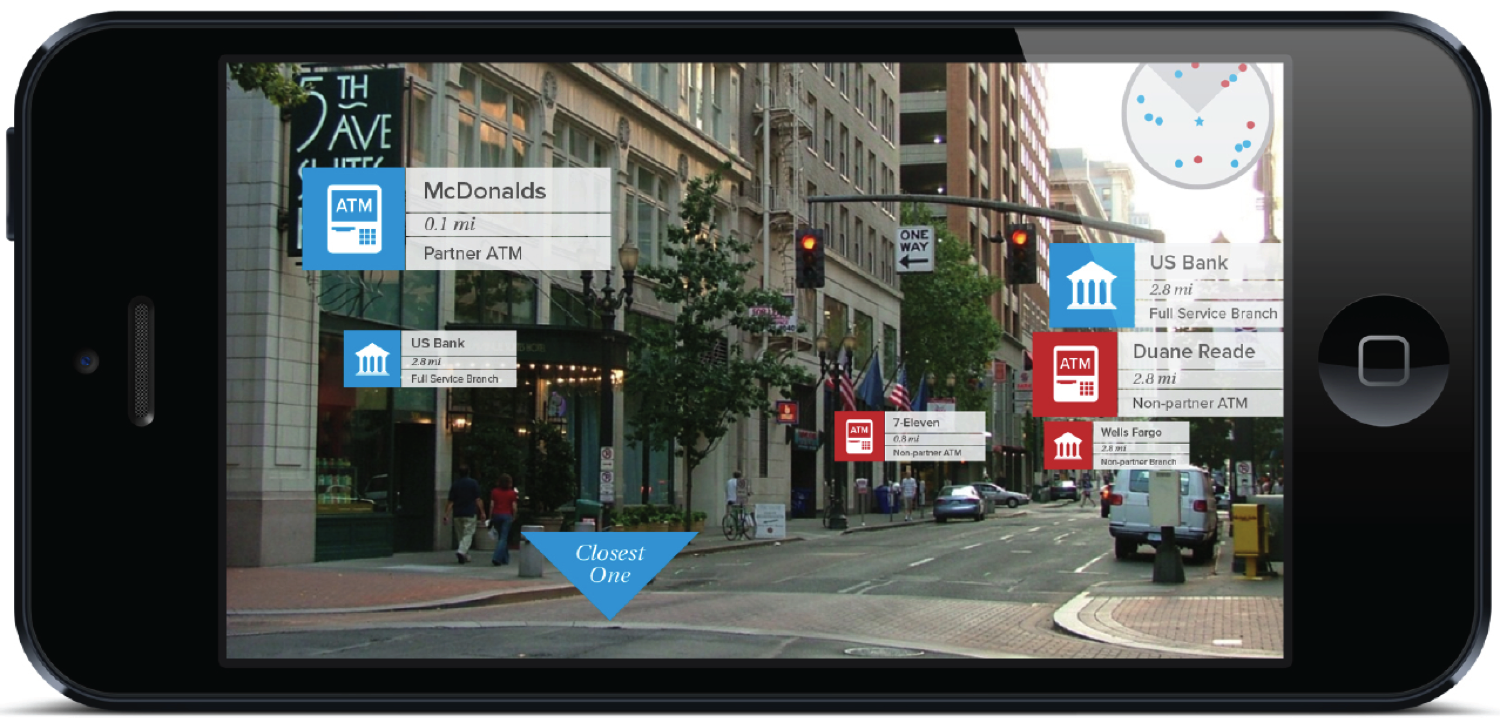
\includegraphics[width=0.85\textwidth]{figs/1-AugmentedReality.png}
\caption{Imagen sobre una aplicación de realidad aumentada.}
\label{fig:1-AugmentedReality}
\end{center}
\end{figure}

La aumentación web por tanto tiene un cometido muy similar al de la realidad aumentada, donde en este caso basándose en un sitio web concreto se realizan modificaciones virtuales, es decir, el sitio web real no se modifica, pero si se hace a la hora de presentarla al usuario con tal de satisfacer sus necesidades.

Estas necesidades pueden ser diferentes, pero habitualmente lo que se trata de mejorar es la focalización en las cosas que se quieren trabajar en el sitio web. Para ello se retiran elementos que no son necesarios y se cambian de sitio otros (dependiendo de la importancia que tengan para la labor que se esté desarrollando sobre ese sitio web).

En la arquitectura WWW (World Wide Web) existen dos agentes principales: el proveedor de contenidos (el servidor web) y el que renderiza (como por ejemplo el navegador web). El proveedor proporciona un contenido, habitualmente el mismo (o similar para todos los usuarios), que él considera adecuado para la mayoría de visitantes. Aun así las necesidades de todos los usuarios no son las mismas y puede que ese sitio web no permita realizar una navegación completamente satisfactoria en un usuario final.

Para resolver estas necesidades existen dos opciones. La primera es que lo haga el/los \emph{webmaster}. El webmaster será capaz de resolver las necesidades de cada uno de los usuarios ofreciendo contenido diferente acorde a esas necesidades, una labor costosa. La segunda solución es delegar parte de la responsabilidad al usuario.

Para ello se utilizan \emph{plugins}, extensiones, \emph{userscripts}, etc. Actualmente, la mayoría de navegadores admiten este tipo de tecnologías.


\section{Sobre WebMakeUp}
\label{sec:SobreWebMakeUp}

Las tecnologías que existen requieren de bastantes conocimientos de desarrollo software y conocimientos técnicos como pueden ser \emph{Javascript}, \emph{html} o \emph{css}. Habitualmente los usuarios carecen de ese tiempo, tanto para aprenderlos, como para desarrollarlos posteriormente.

De esta problemática surge la solución de realizar un editor DIY (\emph{Do-it yourself}), es decir, que un usuario sin necesidad de grandes conocimientos pueda realizar una aumentación. Con ella se pueden cubrir sus necesidades al acceder a un sitio web concreto. Mediante este editor bautizado como \textbf{WebMakeUp} se pueden crear \emph{mods} de un sitio web.

Un mod de un sitio web consiste en una modificación del contenido. Este contenido lo ofrece el proveedor del sitio web al que se accede. Los cambios que se pueden afectan al contenido Document Object Model (a partir de ahora DOM) HTML \footnote{¿Qué es el DOM HTML?: \url{http://www.w3schools.com/js/js_htmldom.asp}}, estilo o forma CSS, o interacción mediante Javascript. 

El contenido se relaciona con el concepto de Widget, es decir, un "trozo" de un sitio web, que puede abarcar desde toda la página, hasta un simple enlace, imagen, vídeo, etc. Un Widget puede tener o no interacción, y asociado a él va un estilo concreto. El usuario crea, modifica o destruye widgets para poder realizar una aumentación.

\begin{figure}
\begin{center}
\subfloat[TV Guía original]{
	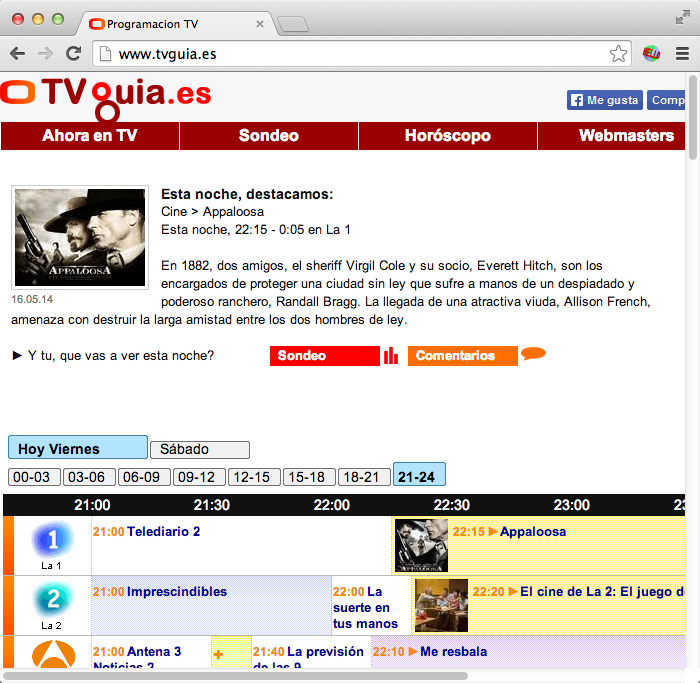
\includegraphics[width=0.5\textwidth]{figs/1-TVGuiaBefore.png}
	\label{fig:1-TVGuiaBefore}
}
\subfloat[TV Guia modificada]{
	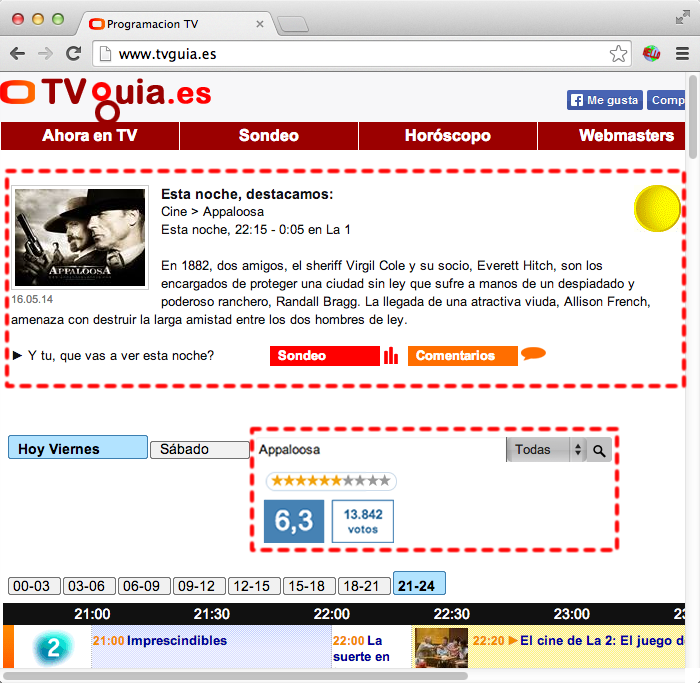
\includegraphics[width=0.5\textwidth]{figs/1-TVGuiaAfter.png}
	\label{fig:1-TVGuiaAfter}
}
\caption{\emph{www.tvguia.es} antes y después de ser modificada: se elimina el canal \emph{La 1} y se añaden ratings de filmaffinity sobre la película de la noche.}
\label{fig:1-TVGuia}
\end{center}
\end{figure}

Por ejemplo, en la Figura \ref{fig:1-TVGuia} se muestra la página web \url{www.tvguia.es} que ofrece la programación de las cadenas de televisión, donde se destaca en la parte superior la película de la noche. Mediante WebMakeUp se ha hecho un mod, donde se elimina la programación del canal \emph{La 1} y se añade el \emph{rating} (o puntuación) que le dan en \emph{www.filmaffinity.com} a la película destacada.

Gracias a este mod, se puede evitar ver información que no interesa (como puede ser la programación de un canal en concreto). También añadir información de otros sitios webs que interese dependiendo del contenido que sale en la propia web (como puede ser en este caso puntuación de la película obtenida de Filmaffinity).

El editor WebMakeUp se encarga de facilitar al usuario esta tarea ofreciendo un Lenguaje Específico de Dominio (\emph{Domain Specific Language}, a partir de ahora DSL), que trata de describir mediante un lenguaje lo más natural posible para un usuario final la manera de concebir una aumentación web.

Para definir este DSL hay que basarse en varias premisas. Una de ellas es la de poder realizarla en poco tiempo, en un \emph{coffee-break} o tiempo de tomar el café, unos 30 minutos. Estos coffee-breaks están condicionados a interrupciones por parte de compañeros de trabajo. Asimismo, los usuarios finales suelen ser bastante impacientes, quieren ver resultados rápido y sin necesidad de realizar grandes esfuerzos. También se ha tenido en cuenta el poco conocimiento del usuario, no conoce conceptos de programación, ni tiene la necesidad de ello, por tanto el editor tiene que ser lo más intuitivo posible y alejarse de la programación tratando de acercarse al lenguaje más afín al usuario.

Como buena muestra de estas propiedades, se ha desarrollado un pequeño vídeo\footnote{Vídeo de ejemplo de realización de una aumentación en WebMakeUp: \url{http://onekin.org/downloads/
public/WebMakeup/video.mov}} que describe cómo se realiza la aumentación web de la Figura \ref{fig:1-TVGuia}.

\section{Sobre el proyecto}
\label{sec:SobreProyecto}

Este documento refleja el trabajo realizado en tres áreas muy concretas de la aplicación WebMakeUp. Se han dividido en tres tareas, pero para garantizar la completa comprensión de las mismas y dado que tienen relación con el resto de la herramienta desarrollada, también se mencionarán otros aspectos a lo largo del propio documento.

El primero de los ámbitos en los que se trabaja está ubicado en las fases iniciales del proyecto. En ella hay que \textbf{buscar y analizar herramientas orientadas al usuario final} que tuvieran cabida con el concepto que se quería trabajar WYSIWYG (\emph{What You See Is What You Get}, es decir, que lo que ves es lo que vas a obtener). Para ello se tiene que investigar y analizar herramientas de desarrollo y editores orientados a usuarios finales (por ejemplo, Photoshop, muy relacionado con el concepto WYSIWYG). El objetivo, por tanto, es tratar de ajustarse a lo que se necesita, para poder describir el DSL y a su vez hacerlo \emph{user-friendly}, sencillo para el usuario.

Otra de las tareas importantes, que abarca gran parte del proyecto, \textbf{es la de describir las animaciones (o interacciones) de la aumentación} (conocido en WebMakeUp como modelo de orquestación u \emph{Orchestration}). Se opta en una primera versión por realizarlo de una manera gráfica mediante diagramas de transición de estados (\emph{State Transition Diagram}, a partir de ahora STD). Pero, finalmente, esta metodología no se ha decidido aplicar en base a estudios con usuarios finales, dada la complejidad que generaban. Para ello se decidió sustituir por la técnica basada en blinks (pestañeo), donde un Widget tiene dos estados \emph{enable} (mostrándose) o \emph{collapse} (ocultándose). La interacción con otros Widgets provocará esos blinks, alternando de un estado a otro.

El tercer aspecto, consiste en \textbf{transformar la aumentación en una extensión para el navegador Google Chrome}. Esto se hace a partir del modelo existente en el editor WebMakeUp. El usuario a medida que va trabajando con el editor, de manera interna se va generando un modelo de datos. El objetivo de esta tercera tarea es la de a partir de ese modelo generar una extensión funcional de Google Chrome. Con ello se evita tener que programar o conocer la plataforma. 

Cabe destacar que el proyecto tiene una dificultad clara en el desarrollo y la investigación, dada la temática, que es muy novedosa. Aun así, a lo largo del proyecto se trabajan otros valores añadidos, que se irán desglosando a lo largo del propio documento. Por ejemplo, metodologías ágiles de desarrollo, trabajos con herramientas colaborativas, etc.

\subsection{Estructura de la memoria}

La estructura de la memoria se divide en diferentes capítulos.

En el Capítulo \ref{cha:Antecedentes} se habla de los antecedentes del proyecto. Se comentan aspectos del marco de conocimiento que requiere este proyecto, las técnicas o herramientas que hay que conocer para el desarrollo del mismo, y la metodología de trabajo en grupo que existía.

El Capítulo \ref{cha:DOP} trata sobre los objetivos del proyecto. Se comentan las tareas y objetivos que se han definido para el cumplimiento del proyecto. A su vez, también se hace una breve mención de qué objetivos no se trataron y quedan como trabajo futuro.

El Capítulo \ref{cha:interacciones} habla sobre el desarrollo de la tarea introductoria de búsqueda de editores para ver cómo se podrían reflejar las aumentaciones de manera gráfica. Esto dará pie a la tarea de cómo reflejar las interacciones de aumentación, explicando las dos ideas que se han trabajado. La inicial, basada en diagramas de transición de estados, y la actual, basada en blinks.

El Capítulo \ref{cha:generador} se habla sobre el transformador de WebMakeUp. La idea de las interacciones con STDs, se utiliza para generar una extensión de Google Chrome a partir del modelo que proporciona WebMakeUp.

Además de lo que es el propio desarrollo del PFG, en el Capítulo \ref{cha:gestion} se comentarán los aspectos relacionados con la gestión del mismo, donde tienen cabida distintos aspectos de gestión, planificación, seguimiento y control, gestión de riesgos, de calidad, etc. Se observará cómo de satisfactoria ha sido la planificación y en qué medida se han cumplido los objetivos.

Se extraerán conclusiones en el Capítulo \ref{cha:conclusiones}, comentando cuáles han sido los objetivos, las enseñanzas y el trabajo futuro o las limitaciones del PFG.

Por último, comentar que existen diferentes anexos que complementan la lectura y completa la compresión del PFG. El Anexo \ref{sec:ActasDeReunion} presenta un acta de reunión de las múltiples que hay a lo largo del PFG. El Anexo \ref{sec:HerramientasGestion} se mencionan las diferentes herramientas de gestión que se han utilizado. El Anexo \ref{sec:ManualWebMakeUp} ofrece un breve manual de uso de WebMakeUp. Finalmente, el Anexo \ref{sec:CJS} describe ConstraintJS, una librería para implementar restricciones y máquinas finitas de estado (FSM) en Javascript.
\chapter{Antecedentes}
\label{cha:Antecedentes}


\section{Marco de conocimiento}

La base del desarrollo de este proyecto se centra en dos de las asignaturas cursadas a lo largo del Grado en Ingeniería Informática, que son Gestión Avanzada de la Información (GAI) y Desarrollo Industrial del Software (DIS).

En la primera de ellas, se estudian conceptos relacionados con la Web 2.0, la aumentación web. En la segunda de ellas, se estudian conceptos relacionados con el desarrollo dirigido por modelos.

También se ha requerido la necesidad de nociones aprendidas en Interacción Persona Computador, donde se abarcan aspectos relacionados con el desarrollo para usuarios finales y la idea del DIY (\emph{Do-it yourself}).

Una aumentación web, al igual que cualquier aplicación convencional, se divide en dos fases. Por un lado, la fase de edición de la aumentación, que es cuando se está describiendo cómo va a ser esa aumentación. Esta fase equivaldría a todo el desarrollo software, donde se analiza, desarrolla, implementa y verifica una aplicación. Por otro lado, está la fase de despliegue, que es una vez hecha la aplicación, donde se pone en marcha y utiliza.

Es importante diferenciar estas dos fases, dado que en este proyecto se ha trabajado en ambas, y lo que se genera en la fase de desarrollo se refleja posteriormente en la fase de puesta en marcha.

En una aumentación web existen diferentes artefactos. Hay widgets, que son componentes o "partes" del DOM de un sitio web, como imágenes, texto, tablas, etc. Los widgets colocados en un orden concreto ofrecen un sitio web en el que el usuario navega. Estos widgets además disponen de características de interacción, es decir, al interactuar con ellos se producen eventos que hacen cambiar el comportamiento de otros widgets. Por ejemplo, al hacer doble clic sobre un widget, se puede hacer para que se oculte algo. A esto en el proyecto se le llama modelo de orquestación.

Para reflejar estos aspectos, se requiere por un lado en el editor una manera de representarlos de cara al usuario, y por otro lado, una representación interna en forma de datos con la que trabajar con ellos, consiguiendo generar la extensión resultante en base al modelo (desarrollo dirigido por modelos).

\section{Marco instrumental}

Dentro del proyecto, se trabaja fundamentalmente con tres herramientas o tecnologías. Por un lado, tanto el desarrollo del propio editor, como el código generado está desarrollado prácticamente en Javascript. Cabe destacar que Javascript es el lenguaje utilizado para el desarrollo de extensiones de Google Chrome y por tanto la elección de Chrome implicaba disponer de conocimientos de Javascript. De igual manera, el propio WebMakeUp es un instrumento utilizado en el PFG. Este proporciona el framework de representación del modelo de datos (tanto el del usuario final mediante la interfaz del editor, como el modelo interno, con la representación para cargar, guardar o exportar aumentaciones realizadas en WebMakeUp).

\subsection{Javascript}

Javascript es el lenguaje del lado cliente en navegadores web más utilizado. Existen alternativas cómo VisualBasic Script (prácticamente obsoleto en navegadores web), Flash (de Adobe) o Silverlight (de Microsoft).

Javascript es un lenguaje interpretado, es decir, es código fuente que se interpreta en tiempo de ejecución. Esto permite, entre otras cosas, que sea independiente de la plataforma donde se ejecuta (Platform Independent). Aspecto muy útil en la web, dado que existen diferentes navegadores, sistemas operativos,etc. e Internet es un punto de encuentro para todos ellos.

Javascript al ser interpretado, requiere de un motor que lo interprete y ejecute ese código. Actualmente todos los navegadores modernos disponen de uno, pero no todos interpretan el código de la misma manera. De ahí surge la necesidad de crear un estándar como \emph{ECMAScript}. Los navegadores deben aceptar ese estándar. Si el código está escrito cumpliendo con \emph{ECMAScript} se garantiza que funciona en todos los navegadores que cumplan con el estándar.

\subsection{Google Chrome}

Google Chrome es el navegador web que se decidió utilizar en el proyecto WebMakeUp. Google Chrome es un navegador de propósito general desarrollado por Google.

Chrome, entre sus múltiples características, permite la modificación de sitios webs en el lado cliente mediante aplicaciones conocidas como extensiones. Estas extensiones están desarrolladas en Javascript.

En el apartado \ref{sec:PSM-GoogleChrome} se comenta más en profundidad el funcionamiento de Google Chrome.

\subsection{WebMakeUp}

WebMakeUp es un editor desarrollado como extensión de Google Chrome. Este editor se integra dentro del propio navegador y el trabajo con él es dentro del propio navegador.

El objetivo de WebMakeUp es el de funcionar como un editor de mods de sitios web. Hacer \emph{modding} sobre un sitio web se podría asemejar a hacer \emph{tunning} en un automóvil, donde el coche sigue siendo el mismo que el de fábrica, pero donde se le añaden, retiran o sustituyen componentes haciéndolo más agradable al usuario que lo va a utilizar.

Los componentes en WebMakeUp se llaman widgets. Los widgets además de ofrecer contenido, también disponen de interacciones. Estas interacciones permiten al usuario interactuar con los widgets para que cambien el comportamiento del sitio web, por ejemplo, ocultando y mostrando los propios widgets.

El Canvas tiene como funcionalidad mostrar la aumentación de una manera gráfica donde se muestran los widgets y las interacciones entre ellos. Se podría decir que uno de los objetivos primordiales de WebMakeUp es el de realizar una herramienta sencilla, usando como metáfora otra herramienta ya conocida. En este caso, el Canvas se inspira en el lienzo de Photoshop que es donde se refleja de manera gráfica y con un simple vistazo toda la edición de una fotografía. En este caso, WebMakeUp y su interfaz reflejan toda la aumentación en un simple vistazo.

Por tanto, WebMakeUp funciona en tiempo de edición, es decir, presenta un editor para poder describir las aumentaciones.

\section{Marco laboral}

La idea de realizar un editor como WebMakeUp surge del grupo Onekin\footnote{Sitio web del grupo Onekin: http://www.onekin.org/}. El grupo Onekin es un grupo de investigación localizado en la Facultad de Informática de San Sebastián que pertenece a la Universidad del País Vasco/Euskal Herriko Unibertsitatea. Este grupo basa sus estudios en diferentes ámbitos de la ingeniería del software, como es la ingeniería de Portlets, líneas de productos software (\emph{Software Product Line} o SPL), en la ingeniería de aplicaciones web y otras más.

Basándose en el lema de Onekin, \emph{``If you want to go quickly, go alone. If you want to go far, go together.``}, que viene a decir, si quieres ir rápido ve sólo, pero si quieres llegar lejos ve unido; el director de proyecto me propuso participar en el proyecto de WebMakeUp.
\chapter{Documento de Objetivos del Proyecto}
\label{cha:DOP}

% Cabecera de pagina con DOP
\chaptermark{DOP}

Hay diversos objetivos en este proyecto. Por un lado, la participación en el proyecto WebMakeUp con la realización de tres tareas. Por otro lado, a nivel personal la realización de un proyecto con el que aprender a utilizar diferentes tecnologías. Estas tecnologías servirán tanto para la realización del producto como del proyecto.

Estas tres tareas se han ido definiendo a medida que el proyecto iba progresando, dado que al ser un proyecto de investigación, el objetivo va cambiando a medida que se va determinando por dónde avanzar. Por tanto se podría decir que en un inicio los objetivos no estaban claramente definidos y se han ido encaminando durante el transcurso del mismo. De igual manera, al tratarse de un desarrollo ágil no toda la funcionalidad desarrollada se ha puesto en marcha, si no que se han podido descartar partes a lo largo del propio desarrollo.

La primera de las tres tareas de desarrollo viene dada en los comienzos de WebMakeUp. En la primera fase del desarrollo, se requiere una labor de análisis del contexto. Hay que buscar una manera sencilla de cara al usuario de representar la zona de trabajo y el cómo se van a disponer de las herramientas para que fuese \emph{user-friendly} (sencillo para el usuario final). Para ello se tuvo que hacer un estudio de editores de diferente tipo con tal de encontrar alguno que pudiera coincidir con lo que se quiere describir en WebMakeUp, una aumentación web.

La segunda de las tareas del proyecto viene a partir de la necesidad de trabajar con las interacciones entre widgets. Un usuario, al interaccionar con el sitio web, genera eventos. Estos producen cambios de contenido. En primer lugar, se ha trabajado con diagramas de transición de estados (STD). Cada uno de estos estados representa una disposición de los widgets y las transiciones entre estados se hacen en base a eventos (Apartado \ref{sec:modeloSTD}). Posteriormente tras pruebas con usuarios finales se decide cambiar de representación y utilizar un sistema basado en blinks (Apartado \ref{sec:modeloBlinks}).

La tercera de las tareas y la más importante una vez teniendo un primer prototipo funcional de la herramienta es reflejar esa aumentación. A partir de un modelo de datos que proporciona el editor generar una extensión de Google Chrome con la aumentación descrita. Por tanto se trata de un desarrollo en base a modelos descritos en un lenguaje específico de dominio (DSL). Para ello se definen algoritmos y técnicas que hay que verificar meticulosamente.

Al igual que como objetivos se plantean estas tareas, también hay otros objetivos transversales en la realización de este proyecto. Entre ellos destacan: el aprendizaje de cómo funciona un proyecto de investigación, el trabajar con documentación colaborativa, desarrollo con control de versiones (en este caso GIT) y metodologías ágiles basada en prototipos, gestión de tareas mediante una herramienta colaborativa, gestión de la calidad en el desarrollo, aprendizaje de patrones de diseño, etc. En general, diferentes técnicas que complementan un proyecto innovador.

Otro de los posibles objetivos que se podía haber desarrollado en este proyecto es el desarrollo multiplataforma de las aumentaciones realizadas. Esto implica disponer de múltiples generadores, uno por cada navegador al que se quiera extender estas aumentaciones; o disponer de un tipo de extensión compatible con todas las plataformas, como por ejemplo los \emph{userscripts}\footnote{Descripción de userscripts: http://en.wikipedia.org/wiki/Userscript}.
\chapter{Modelo para las interacciones de aumentación}

\label{cha:interacciones}

\chaptermark{Interacciones de aumentación}

Las interacciones de aumentación constituyen la parte dinámica de la aplicación WebMakeUp. Las interacciones se realizan entre el usuario y los widgets. El usuario, a medida que va trabajando con el sitio web, puede generar diferentes tipos de eventos Javascript (clic-ar, pasar el ratón por encima, escribir en un widget, arrastrar y soltarlo, etc.).

En una aumentación web, además de añadir y quitar contenido de un sitio web, se le puede dotar de interacción usuario-widgets, haciéndolo más dinámico. Por ejemplo, puede existir un botón que al pulsarlo muestre u oculte cierto contenido, o que al escribir en un cuadro de texto si la palabra está mal formada se muestre otro widget en color rojo indicando que hay un error. Todo esto y mucho más se hace mediante Javascript, que es el encargado en el lado cliente de todo el dinamismo.

El problema surge cuando un usuario para realizar una aumentación tiene que aprender a programar la escucha de estos eventos (para saber cuándo se producen). Pero no solo eso, sino que también las funciones que se tienen que realizar cuándo este evento se produce (concepto conocido como manejador o handler).

Por tanto, en WebMakeUp surge la necesidad de tener un modelo de interacciones de aumentación que se encargue de gestionar todo este proceso. Esto evitará que el usuario, por un lado, tenga que aprender Javascript, y por otro lado, disponer de una cantidad de tiempo considerable para desarrollar la aumentación.

Pero antes de ello, es necesario saber cómo se va a estructurar el editor WebMakeUp. De esta idea surge la primera tarea de WebMakeUp, estudiar diferentes herramientas de edición existentes en el mercado (Apartado \ref{sec:editoresRetoque}). Así se puede representar, por una parte, el trabajo de los widgets (línea de investigación que no se ha realizado en este PFG), y por otra, representar las interacciones entre widgets (que se ha realizado en gran medida en este PFG y es en la que se centrará este capítulo).

Para la representación del modelo de interacciones, se propuso realizarlo en base a diagramas de transición de estados (que se explicará en el Apartado \ref{sec:modeloSTD}). Aunque, tras pruebas con usuarios finales de la aplicación, se decide desechar la idea y sustituirla por otra más sencilla basada en blinks (que se explica en el Apartado \ref{sec:modeloBlinks}).

\section{Editores de retoque}
\label{sec:editoresRetoque}

El estudio de editores de retoque tiene diferentes finalidades:
\begin{itemize}
\item{Permite conocer las herramientas que están presentes en el mercado y que utilizan usuarios finales habitualmente. Esto puede ayudar a encontrar un equilibrio entre el lenguaje de programación y el lenguaje que conoce el usuario final.}
\item{Buscar cómo se representan algunos aspectos técnicos y complejos para un usuario final. Ya sea utilización de iconos, el entorno de trabajo al que está habituado el usuario final, etc.}
\item{Buscar si existen herramientas similares a lo que con WebMakeUp se tenía intención de hacer.}
\item{Descartar ideas complejas, centrándose en diseñar un DSL (lenguaje específico de dominio) sencillo para un usuario, donde el objetivo es que prácticamente cualquier usuario de sitios webs pueda diseñar una aumentación.}
\end{itemize}

Para marcar un primer objetivo, hay que buscar información general sobre diferentes editores de uso común. Para ello hay que basarse en editores donde el propósito era igual que el de WebMakeUp, trabajar sobre un artefacto ya existente y crear un mod a partir de él. Para ello se tiene que buscar herramientas en las que basar la metáfora, con tal de poder decir \emph{si sabes utilizar X herramienta, sabes utilizar WebMakeUp}.

En el cuadro \ref{tab:EditoresRetoque} se muestran algunos de los editores que se estudiaron donde las principales características a valorar eran la relación que se pudiera asociar entre la interfaz del editor y las necesidades de mostrar widgets e interacciones entre ellos que tenía WebMakeUp.

\begin{table}
\begin{center}
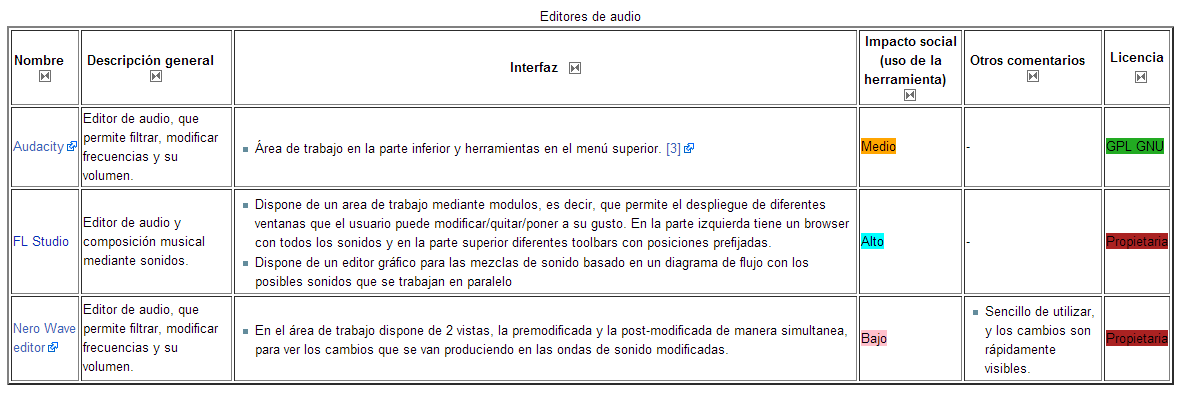
\includegraphics[width=0.95\textwidth]{figs/4-EditoresDeAudio.png}
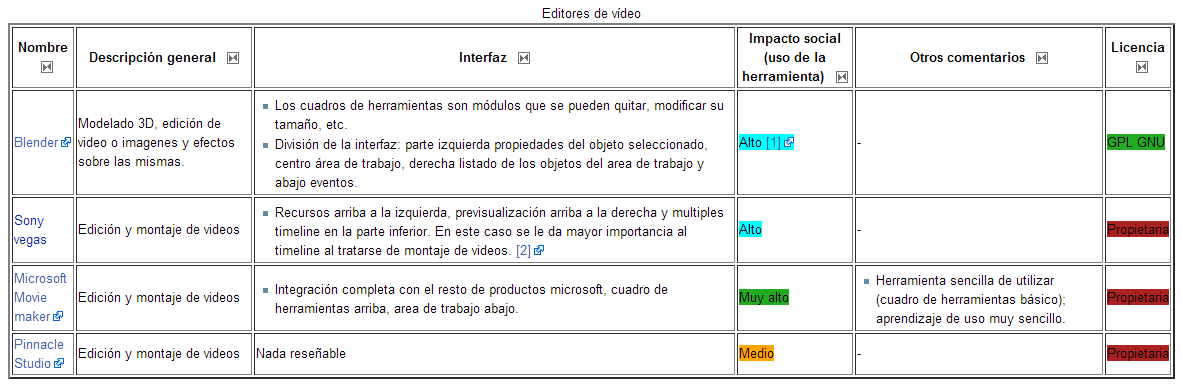
\includegraphics[width=0.95\textwidth]{figs/4-EditoresDeVideo.png}
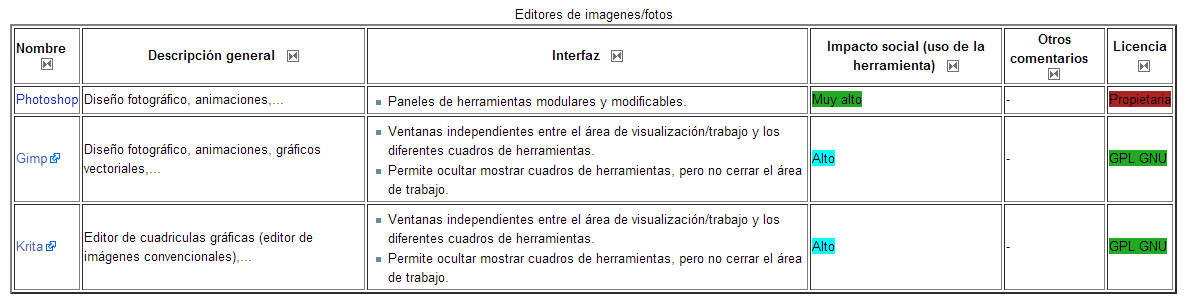
\includegraphics[width=0.95\textwidth]{figs/4-EditoresDeImagenes.png}
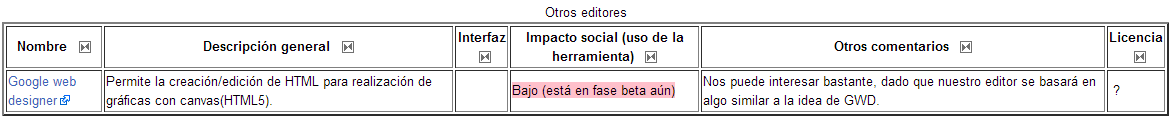
\includegraphics[width=0.95\textwidth]{figs/4-EditoresDeOtroTipo.png}
\caption{Estudio de editores de retoque de uso general (audio, vídeo, imágenes y web).}
\label{tab:EditoresRetoque}
\end{center}
\end{table}

Tras realizar un pequeño estudio general se decide tomar como referencia Photoshop, por varias razones:
\begin{itemize}
\item{Es una de las aplicaciones de edición más conocidas y usadas del mercado.}
\item{El entorno de trabajo es cómodo para el usuario, abre el editor, escoge una imagen, se muestra en el lienzo y a partir de ahí trabaja prácticamente usando sólo el lienzo. En WebMakeUp también se puede realizar eso, abrir el sitio web y a partir de ahí trabajar sobre el Canvas del sitio web de manera gráfica. En la Figura \ref{fig:IDEPhotoshop} de color rojo se refleja el Canvas de Photoshop. Esto se complementa con el artículo \cite{WebSpec}, que recomienda el uso de lenguajes gráficos para la interacción y navegación.}
\item{Disponía de una característica similar a las interacciones. En Photoshop existe una línea temporal para las animaciones, donde a medida que transcurre el tiempo puede ir variando la imagen. En la Figura \ref{fig:IDEPhotoshop} de color verde, se refleja la línea temporal de la animación en Photoshop. En WebMakeUp no existe una línea temporal, pero sí que va variando el contenido y el comportamiento de los widgets del sitio web a medida que el usuario interacciona con él.}
\item{En el lateral izquierdo existen herramientas para la edición de imágenes en Photoshop. En WebMakeUp ese panel puede ser útil para tener herramientas relacionadas con widgets, como por ejemplo un repositorio de widgets.}
\end{itemize}

\begin{figure}
\begin{center}
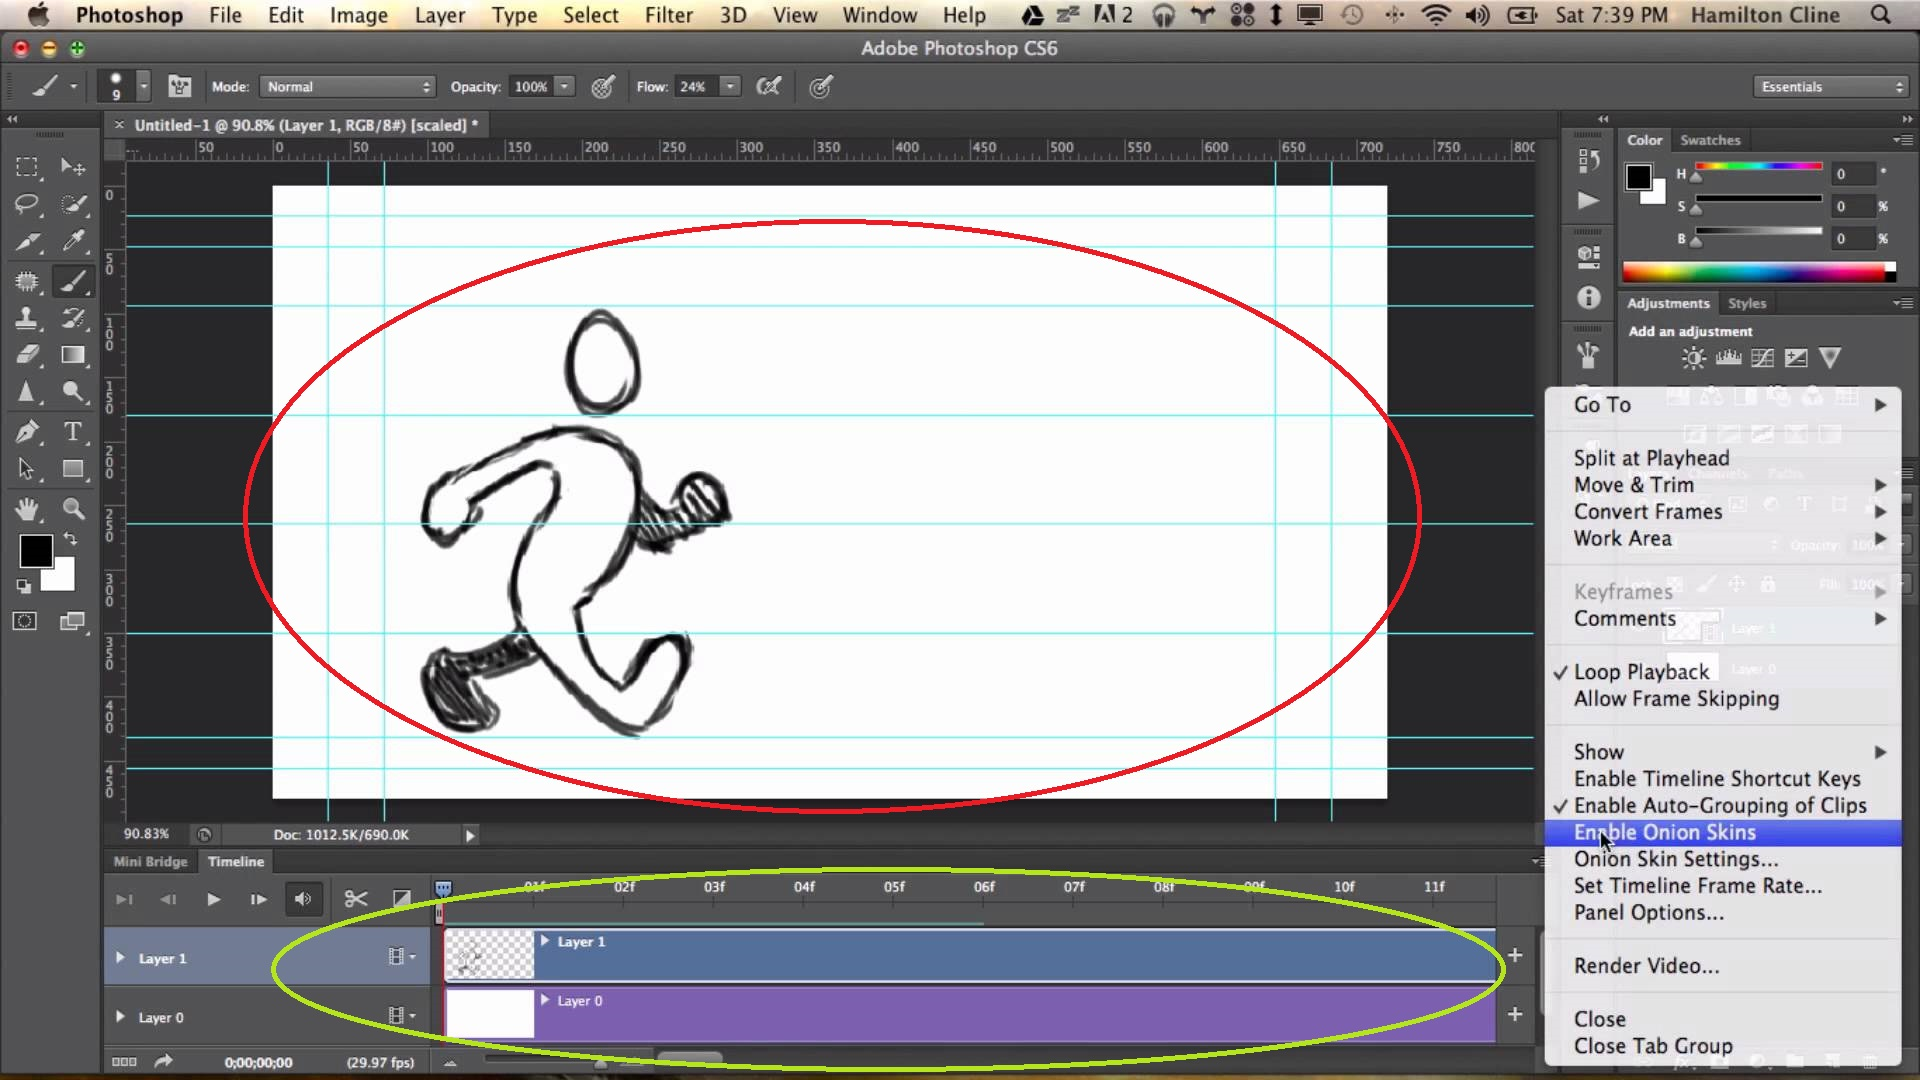
\includegraphics[width=0.95\textwidth]{figs/4-PhotoshopAnimationIDE.png}
\caption{IDE de Photoshop. De color rojo se marca el Canvas y de color verde la animación.}
\label{fig:IDEPhotoshop}
\end{center}
\end{figure}

Una vez definido cuál es el referente en el diseño del entorno de WebMakeUp a seguir, hay que buscar cómo representar las animaciones. Con él, el usuario puede diseñar animaciones sin conocimientos de programación. Este último aspecto limita bastante las opciones de animación que tiene el editor. El incluir aspectos como condiciones, bucles y demás lo haría demasiado complejo.

En el Apartado \ref{sec:modeloSTD} se comenta cuál fue la primera idea de cómo realizar esta representación. En WebMakeUp, tras probarlo con usuarios finales se decide descartar esta representación en favor del uso de blinks (Apartado \ref{sec:modeloBlinks}).

\section{Modelo de diagramas de transición de estados}
\label{sec:modeloSTD}

Para comprender el porqué se decide adoptar el modelo de diagramas de transición de estados (a partir de ahora STD, \emph{State Transition Diagram}) hay que comprender un poco más cómo funcionan las animaciones en Photoshop. En Photoshop las animaciones se producen en base a un evento, el evento temporal. El evento temporal en Photoshop permite cambiar el estado global de la imagen que se está editando, es decir, que existe un evento que hace que se cambie de un estado global a otro.

Pero, ¿qué es el estado global? El estado global en Photoshop lo constituyen, en un instante de tiempo concreto, las capas que están visibles. Las capas en Photoshop equivale a superponer una imagen encima de otra. Habitualmente estas imágenes tienen partes transparentes, que permiten ver la imagen inmediatamente inferior, tal y como se muestra en la Figura \ref{fig:PhotoshopCapas}. Poniendo diferentes capas en diferentes instantes de tiempo se conforman diferentes imágenes y por tanto diferentes estados globales.

\begin{figure}
\begin{center}
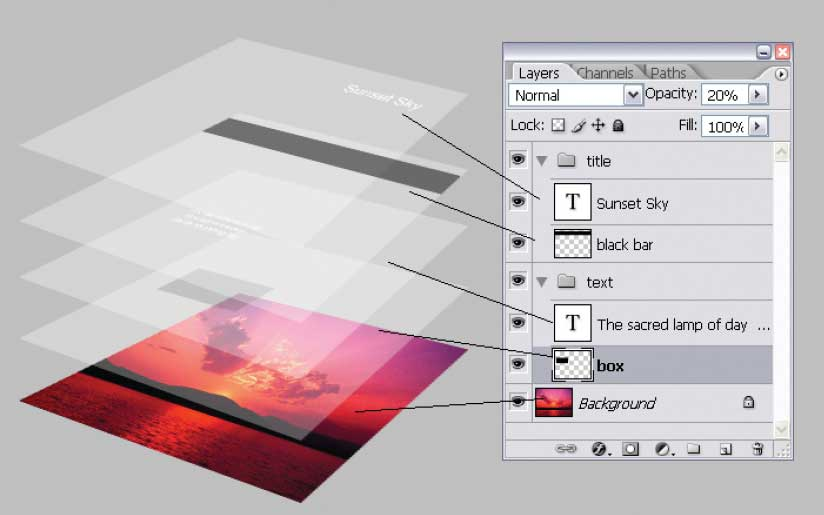
\includegraphics[width=0.35\textwidth]{figs/4-PhotoshopCapas.png}
\caption{Capas de una imagen en Photoshop}
\label{fig:PhotoshopCapas}
\end{center}
\end{figure}


Como se observa en la Figura \ref{fig:PhotoshopTimeline} en cada instante de la línea de tiempo hay diferentes estados globales. En WebMakeUp, se pueden traducir las capas a widgets y los estados de las líneas de tiempo por un STD. Basándose en el artículo  \cite{WhoMovedMyState}, la razón del STD es lógica. Realizar un evento sobre el sitio hace que cambien de estado los widgets, y la suma de los estados de los widgets conforman el estado global (el mismo concepto se utiliza en los sistemas distribuidos y el estado de los nodos \footnote{Gestión de un cluster de IBM PowerVM donde se menciona los 3 posibles estados globales dependiendo del estado de los nodos: \url{http://www-01.ibm.com/support/knowledgecenter/8246-L1T/p7hcgl/cluster.htm}}).

\begin{figure}
\begin{center}
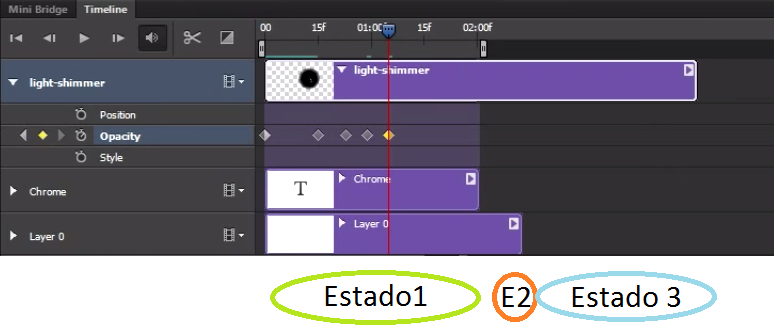
\includegraphics[width=0.75\textwidth]{figs/4-PhotoshopTimeline.png}
\caption{Timeline de Photoshop, donde el estado de las capas a lo largo del tiempo muestra 3 estados globales diferentes.}
\label{fig:PhotoshopTimeline}
\end{center}
\end{figure}

Un STD permite mostrar en un simple vistazo todos los estados posibles de la aplicación y el cómo se llega a esos estados (mediante qué eventos y en qué estado previo).

Pero aún queda por describir qué estados iban a tener los widgets. En un comienzo, como ejemplo de aumentación se toma de referencia una aumentación concreta llamada MyWiki, desarrollada por el grupo de investigación Onekin.

MyWiki es un \emph{userscript} instalable en diferentes navegadores webs (aunque estaba enfocado para Mozilla Firefox). El objetivo de MyWiki es permitir en artículos de Wikipedia\footnote{Sitio web de Wikipedia: \url{http://en.wikipedia.org/}} poder añadir notas y almacenarlas de manera local. En este apartado, se centra únicamente en una funcionalidad muy concreta de cómo está constituida la página web Wikipedia. Tal y como se observa en la Figura \ref{fig:MyWikiAugmentation} existe una nueva pestaña de navegación donde se puede añadir nuestras notas sobre el artículo que se está visitando. Esta pestaña presenta dos estados que pueden resultar interesantes en diferentes tipos de widgets. Estos dos estados son seleccionado y deseleccionado y en uno responde a eventos y en el otro no.

Tomando el ejemplo de MyWiki, además de ser interesante seleccionar y deseleccionar, también hay que tener la opción de ocultar el artículo de XML para mostrar el editor de notas de MyWiki (Figura \ref{fig:MyWikiEditor}).

\begin{figure}
\begin{center}
\subfloat[No augmented Wikipedia]{
	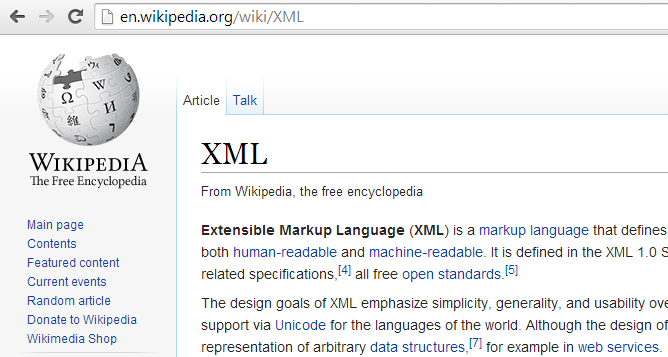
\includegraphics[width=0.47\textwidth]{figs/4-WikipediaXML.png}
}
\subfloat[Augmented with MyWiki]{
	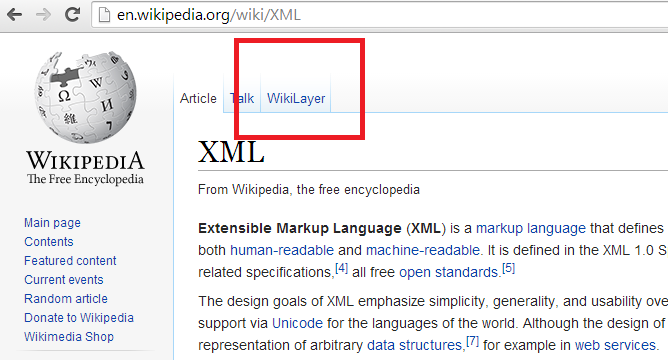
\includegraphics[width=0.47\textwidth]{figs/4-MyWikiTab.png}
}
\caption{A la izquierda artículo de Wikipedia sobre XML. A la derecha el mismo artículo con la aumentación realizada con MyWiki.}
\label{fig:MyWikiAugmentation}
\end{center}
\end{figure}

\begin{figure}
\begin{center}
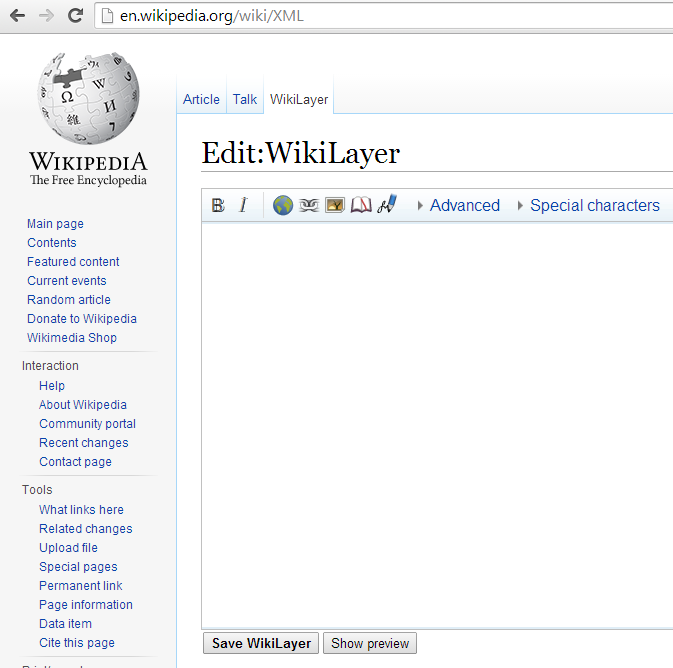
\includegraphics[width=0.45\textwidth]{figs/4-MyWikiEditor.png}
\caption{Editor de MyWiki integrado en Wikipedia.}
\label{fig:MyWikiEditor}
\end{center}
\end{figure}

Los artefactos que se necesitan para describir las interacciones de la aumentación mediante los STD son los siguientes:
\begin{itemize}
\item{Estados: constituido por un nombre (o identificador) y por un listado de los widgets y su estado (selected, deselected o collapsed) en ese estado global.}
\item{Transiciones: constituido por un evento (click, double click, mouseover o mouseout) y en qué widget se produce ese evento para que se dé la transición. Lógicamente, para representar la transición se requiere del identificador del estado origen y del de destino.}
\end{itemize}

Una vez definido los artefactos con los que se va a trabajar solo queda por describir cómo se ha hecho. Para ello hay que hacer un estudio, por un lado de herramientas que permitan describir de manera gráfica, y por otro lado, cómo representar internamente esas interacciones para la futura generación de la extensión con la aumentación \emph{ready to use} (lista para instalar y usar).

Sobre la generación de la extensión se habla en el Capítulo \ref{cha:generador}. En él se menciona el cómo se decide usar una librería llamada ConstraintJS con una sencilla API para trabajar con STDs (ver Anexo \ref{sec:CJS}). En consecuencia, este apartado se centra en cómo se representar de manera gráfica y cómo interactuar entre el diagrama STD y el Canvas.

Para ello, antes de nada, es conveniente estudiar cómo es la primera versión funcional de WebMakeUp. En la Figura \ref{fig:WebMakeUpVer1} se muestran dos paneles, uno izquierdo y otro inferior. El panel izquierdo contiene un repositorio de widgets. Estos se arrastran sobre el Canvas (que es la instancia del sitio web, en este caso Wikipedia). Por otro lado, el panel inferior es donde está el STD. Este está programado íntegramente usando una librería para dibujar diagramas de diferente tipo usando la tecnología Canvas HTML5 (no confundir con el Canvas de WebMakeUp) llamada GoJS. Canvas HTML5 es una nueva característica de HTML5 que permite crear dibujos sobre un lienzo. En el lienzo se dibujan diferentes tipos de objetos (formas geométricas, textos, degradados, imágenes,...) mediante el uso de Javascript.

\begin{figure}
\begin{center}
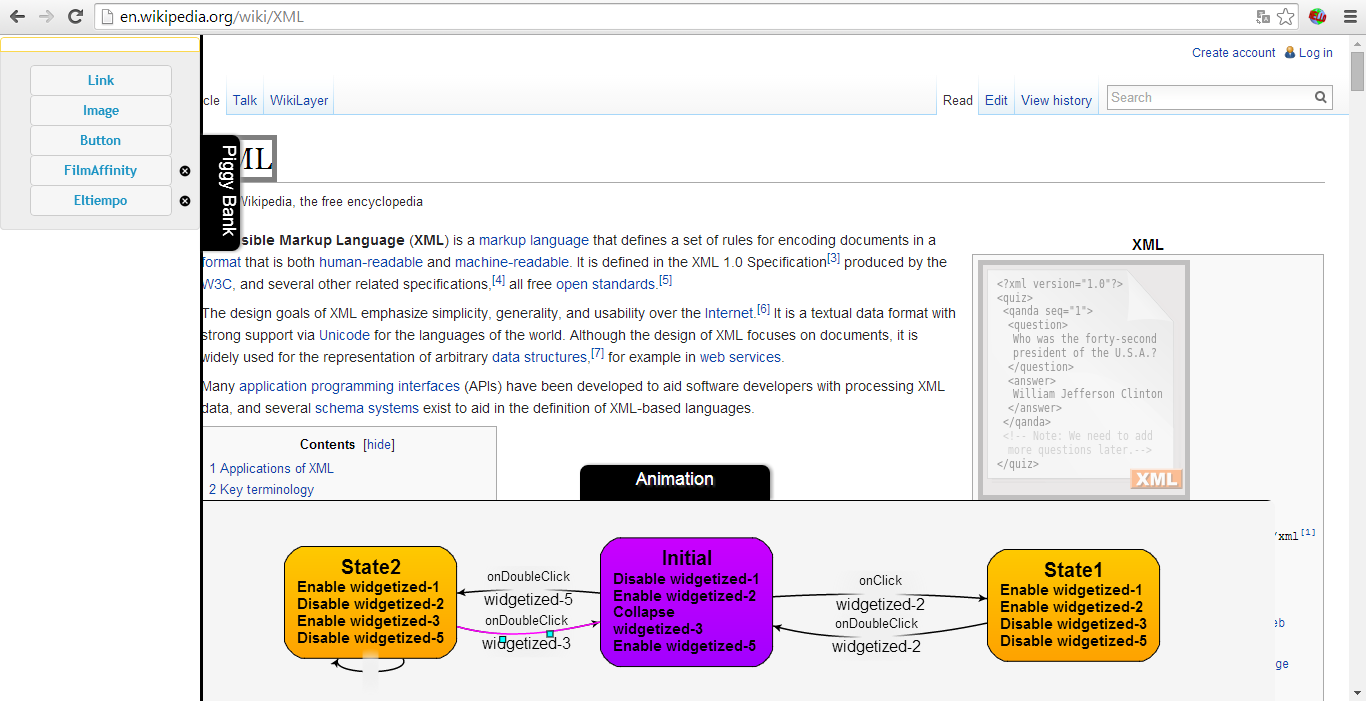
\includegraphics[width=0.95\textwidth]{figs/4-WebMakeUpVer1.png}
\caption{Editor WebMakeUp realizando una aumentación en \url{www.wikipedia.org.}}
\label{fig:WebMakeUpVer1}
\end{center}
\end{figure}

\subsection{GoJS - Librería de gráficas HTML5}
\label{sec:Interacciones-GoJS}

GoJS, tal y como lo describen en su sitio web\footnote{Sitio web de: \url{ http://www.gojs.net/latest/index.html}}, es una librería Javascript para implementar diagramas interactivos en diferentes navegadores actuales. Se basa en nodos, links y grupos para la creación de estos diagramas. Es fácilmente configurable mediante plantillas.

En su sitio ofrecen variedad de ejemplos\footnote{Ejemplo de STD de GoJS: \url{http://www.gojs.net/latest/samples/stateChart.html}} de cómo hacer desde arboles de decisión, EDTs, GANTTs, diagramas de flujo, etc. Se podría decir que es realmente muy configurable, pero la curva de aprendizaje de uso es lenta por dos razones principales:
\begin{itemize}
\item{Al funcionar todo con nodos y links realizar ciertos tipos de diagrama puede ser bastante complejo.}
\item{La API es realmente muy completa, ofrece infinididad de opciones, y la documentación es enorme, pero encontrar cómo se quieren hacer ciertas cosas requiere de búsqueda de alternativas a veces un poco complejas.

Por poner un ejemplo, en los STD de WebMakeUp se requería que el nodo inicial no se pudiera eliminar (ya que al menos se requiere un estado global en una aumentación, el estado inicial). Para realizar esto era necesario definir una capa diferente en el lienzo y crear una plantilla diferente al resto para el nodo inicial. Por tanto, se podría decir mediante este ejemplo que funciona de manera similar a como lo hace Photoshop, con capas. Respecto a las capas no había nada definido en ninguno de los ejemplos, y al ser una librería poco trillada, no era trivial encontrarse con ese método para resolver el problema.}
\end{itemize}

GoJS como se ha comentado, dispone de infinidad de características, y estas son algunas de las que se utilizan en el desarrollo de la interacción basada en STDs:
\begin{itemize}
\item{Es una aplicación desarrollada en Modelo-Vista-Controlador (MVC). El controlador se encarga de gestionar los eventos que se producen en el diagrama (selecciones, borrar nodos o links, etc.). El modelo se encarga de almacenar todos los datos que se generan mientras se trabaja con el editor. La vista se actualiza automáticamente cuando el modelo cambia, lo que favorece mucho el desarrollo ya que los cambios se reflejan automáticamente.}
\item{Las plantillas permiten definir cómo se van a presentar los datos, pero además reflejan qué datos van a estar en el modelo y cómo se va a hacer el \emph{matching} (la concordancia) entre los datos. Por ejemplo, se puede definir que en la vista se muestren los nombres de los widgets presentes en un estado del STD, pero internamente sólo se almacena el identificador.}
\item{GoJS al ser también un editor, en este caso de gráficas en HTML5, permite exportar e importar el modelo de manera sencilla en un objeto JSON, que es como se representan los objetos en Javascript. En el caso de los STDs el JSON que se obtiene es del estilo del que se muestra en la Figura \ref{fig:GoJSModelJSON}}.
\item{De igual manera, como la mayoría de editores dispone de características de edición que son difíciles de implementar, UNDO y REDO (deshacer y rehacer). En la Figura \ref{fig:GoJSTransaction} se muestra cómo GoJS funciona con transacciones, igual que las bases de datos convencionales. Las transacciones se van almacenando y gracias a ello se puede hacer UNDO y REDO.}
\end{itemize}

\begin{figure}
\begin{center}
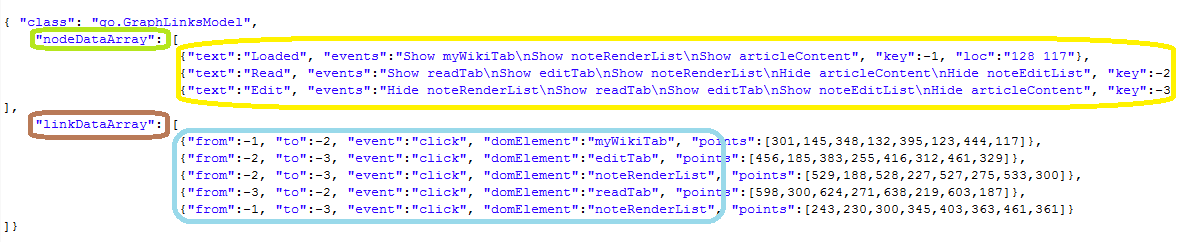
\includegraphics[width=0.95\textwidth]{figs/4-GoJSModelJSON.png}
\caption[Modelo generado por GoJS con información de los estados y transiciones del STD.]{Modelo generado por GoJS con información de los estados y transiciones del STD. De color verde y marrón la declaración de la lista de nodos y transiciones. De color amarillo, la información de los nodos y de azul la de las transiciones.}
\label{fig:GoJSModelJSON}
\end{center}
\end{figure}

\begin{figure}
\begin{center}
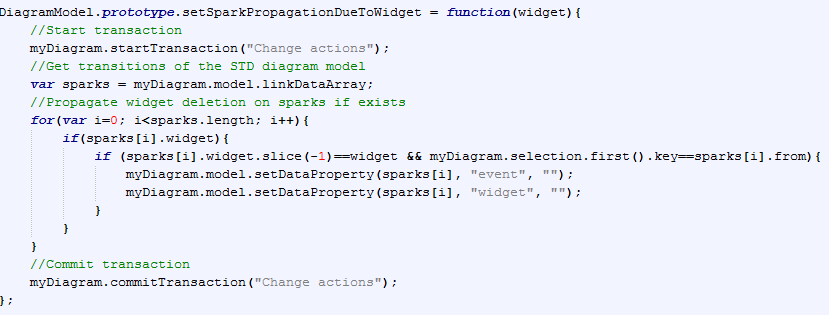
\includegraphics[width=0.95\textwidth]{figs/4-GoJSTransaction.png}
\caption{Funcionamiento de transacciones en el modelo de datos de GoJS.}
\label{fig:GoJSTransaction}
\end{center}
\end{figure}

Estas características permiten que se puedan comunicar mediante una API (basada en restricciones con ConstraintJS) el Canvas y el STD.

Sobre ConstraintJS se habla en el Anexo \ref{sec:CJS}, aunque cabe destacar que es una librería que permite trabajar con restricciones y en base a cambios en esas restricciones ejecutar manejadores (handlers, funciones Javascript) de manera automatizada. 

Por ejemplo, el cambiar el nodo seleccionado en el STD implicaba cambiar de estado de los widgets en el Canvas, tal y como se puede observar en la Figura \ref{fig:WebMakeUpV1NodeSelection}.

\begin{figure}
\begin{center}
\subfloat[Selected state A]{
	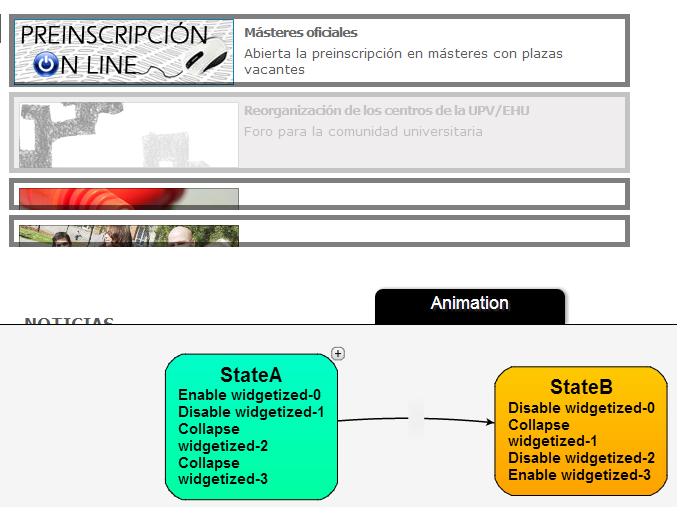
\includegraphics[width=0.47\textwidth]{figs/4-WebMakeUpV1SelectedA.png}
}
\subfloat[Selected state B]{
	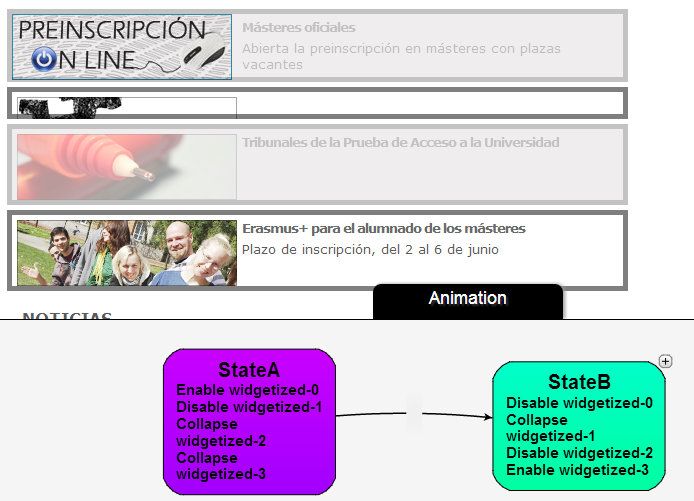
\includegraphics[width=0.47\textwidth]{figs/4-WebMakeUpV1SelectedB.png}
}
\caption{Cambio de estado de los widgets al seleccionar diferentes estados del STD.}
\label{fig:WebMakeUpV1NodeSelection}
\end{center}
\end{figure}

\section{Modelo de blinks}
\label{sec:modeloBlinks}

Tras la realización de un estudio con usuarios finales que no se realizó dentro del PFG, se detectaron muchos aspectos a mejorar. En lo que concierne al PFG, cabe destacar que el diagrama de transición de estados (Apartado \ref{sec:modeloSTD}) era complejo para la mayoría de usuarios por las siguientes razones:
\begin{itemize}
\item{El concepto de estado global es complejo. No se visualiza de manera sencilla la aumentación y lo que se quería aumentar.}
\item{La representación fuera del Canvas resulta confusa. El tener que conocer el nombre de cada uno de los widgets para poder comprender el STD y por tanto las transiciones, hace tediosa la programación de las interacciones.}
\item{El estado deselect no es muy utilizado. Se considera que un estado mostrado y otro ocultado son suficientes.}
\item{No es escalable para los propósitos de los usuarios. Por ejemplo para definir botones que ocultan o mostraban widgets concretos haciendo clic sobre ellos (algo bastante utilizado). Si se definen 3 de este tipo equivale a tener que realizar una máquina de 9 estados. \[x=n^2 / n=numeroDeBotones\] En la Figura \ref{fig:EscalabilidadInteracciones} se refleja la sencillez de los blinks frente a la complejidad de los STD en este caso.}
\end{itemize}

\begin{figure}
\begin{center}
\subfloat[Modelo basado en STD]{
	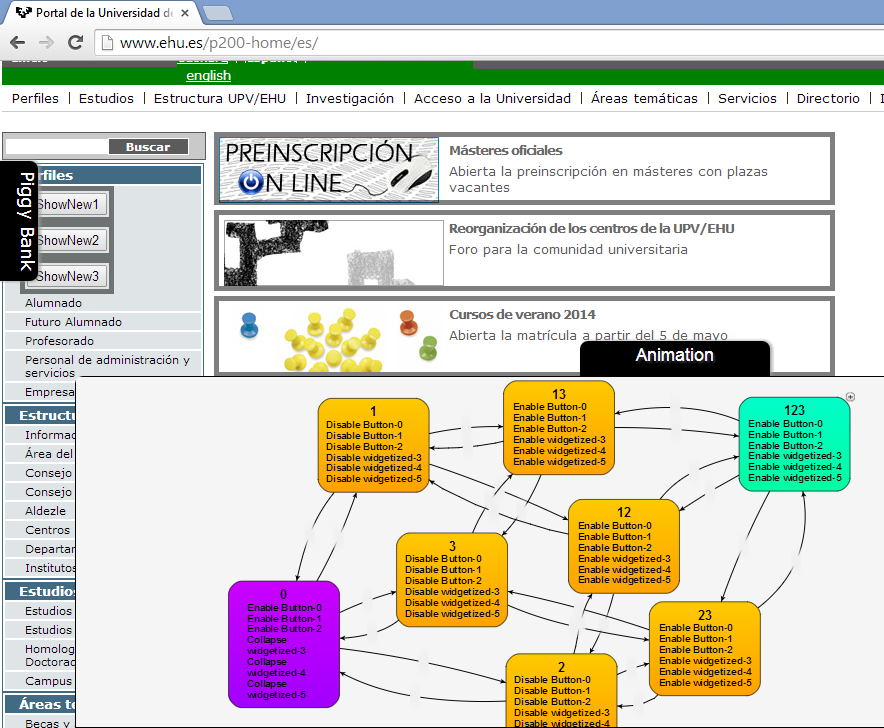
\includegraphics[width=0.45\textwidth]{figs/4-ScalabilitySTD.png}
}
\subfloat[Modelo basado en Blinks]{
	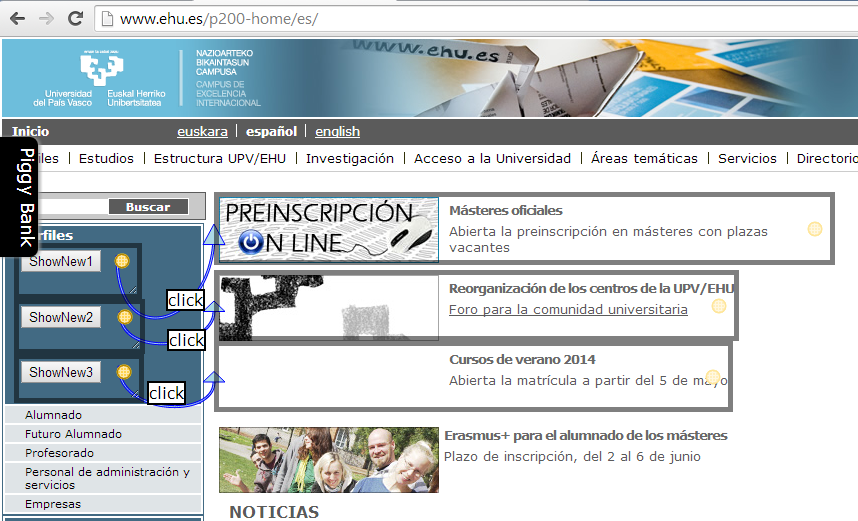
\includegraphics[width=0.45\textwidth]{figs/4-ScalabilityBlink.png}
}
\caption{Comparativa de escalabilidad entre el modelo basado en STD y el modelo basado en blinks.}
\label{fig:EscalabilidadInteracciones}
\end{center}
\end{figure}

Todo este feedback obtenido por parte de los usuarios ha servido para idear otra técnica que es más acorde, solventando los inconvenientes y tratando de aprovechar en la mayor medida posible el trabajo ya previamente realizado.

Esta técnica se basa en un concepto llamado blink, donde los widgets pestañean, es decir, están mostrándose u ocultándose. Ahora no existe un estado global conocido para el usuario, él simplemente tiene que indicar en qué widget se produce el evento para que el widget al que apunta pestañee y cambie su estado de mostrado (\emph{enabled}) a oculto (\emph{collapsed}) o viceversa. Esto se realiza en base a links tal y cómo se observa en la Figura \ref{fig:BlinkLink}.

\begin{figure}
\begin{center}
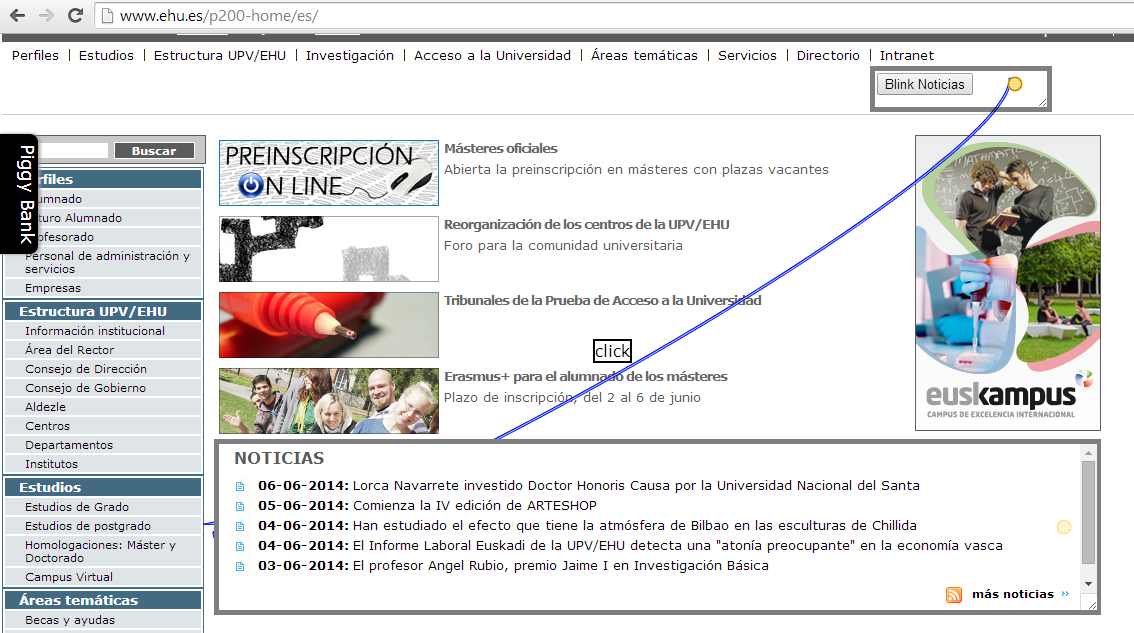
\includegraphics[width=0.55\textwidth]{figs/4-BlinkLink.png}
\caption[WebMakeUp con interacciones mediante el modelo de blinks.]{Editor WebMakeUp con interacciones mediante blinks, con dos widgets conectados mediante un link. El superior es el controlador y el inferior el observador.}
\label{fig:BlinkLink}
\end{center}
\end{figure}

Mediante la técnica de blink por tanto se tienen dos widgets que entran en juego. A uno se le llama el widget observador, que es el que observa si se ha producido un evento en el widget controlador. Si en el widget controlador se produce un evento el observador realiza un blink (es decir, cambia su estado de enable a collapse, o viceversa).

Para ello hay que tener en cuenta un nuevo aspecto, el de eventos opuestos. El evento opuesto es el evento que se tiene que producir para que el observador regrese al estado inicial. En WebMakeUp se definen cuatro eventos: \emph{click}, \emph{double click}, \emph{mouseover} y \emph{mouseout}. Hay que tener en cuenta que mouseover y mouseout están relacionados, es decir, que cuando se pone el cursor sobre un widget se hace un mouseover, y cuando se mueve fuera del widget, se produce un mouseout. Teniendo en cuenta esto, se definen tres eventos y sus opuestos:
\begin{itemize}
\item{Click y su opuesto, que es el propio click. En consecuencia, en el ejemplo de la Figura \ref{fig:BlinkLink}, cada vez que se haga clic en el widget controlador, el observador irá alternandose entre enabled y collapsed.}
\item{DoubleClick y su opuesto, el propio doubleClick.}
\item{Mouseover y su opuesto, mouseout. A este par en WebMakeUp se le llama MouseEnter.}
\end{itemize}

La definición del metamodelo de los blink se puede representar de la manera que se observa en la Figura \ref{fig:BlinkMetamodel}. En el metamodelo hay dos clases, la de widgets y la de blinks. 

La clase \textbf{Widget} representa toda la información del widget. En este caso únicamente se necesita conocer su identificador y el estado inicial. El identificador sirve para crear las relaciones entre widgets. El estado inicial, indica cuál es el estado por defecto del widget. Esto es importante, dado que gracias a definir si un widget inicia en enabled o collapsed, se consiguen generar diferentes tipos de patrones. Esto se explica detalladamente en el Apartado \ref{sec:PatronesBlinks}.

La clase \textbf{Blink} representa la relación de dos widgets (un controlador y un observador). A su vez, hay que tener en cuenta cuál de los tres eventos (DOMEventType) tiene que esperar el observador.

\begin{figure}
\begin{center}
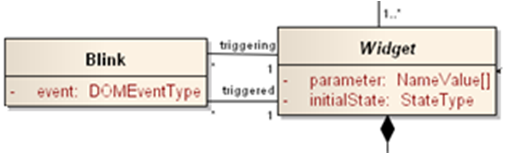
\includegraphics[width=0.45\textwidth]{figs/4-BlinkMetamodel.png}
\caption{Parte del metamodelo de WebMakeUp que representa los blinks.}
\label{fig:BlinkMetamodel}
\end{center}
\end{figure}

Cabe destacar que en este PFG, a diferencia del modelo basado en STD, donde sí se trabajó sobre la presentación al usuario final, en los blinks no fue así. La librería utilizada para dibujar fue WireIt \footnote{Sitio oficial de WireIt: \url{http://neyric.github.com/wireit}} con pequeñas modificaciones adaptándolas a las necesidades de WebMakeUp. Lo que sí se trabajó fue la generación de la extensión de Google Chrome a partir de este nuevo modelo basado en blinks. Esto está desarrollado en el Capítulo \ref{cha:generador}.

\subsection{Patrones de blinks}
\label{sec:PatronesBlinks}

A raíz del paradigma basado en blinks, se pueden definir diferentes tipos de patrones de diseño. Estos patrones de diseño, permiten ayudar a la hora de diseñar interacciones que se pueden dar habitualmente en las aumentaciones web. El usuario simplemente tiene que elegir qué widgets interaccionan y qué patrón de los propuestos siguen. Esto lo que realizará será de manera automatizada añadir las flechas correspondientes que hacen que se cumpla con el patrón deseado. 

Los patrones de diseño juegan con dos aspectos clave en el modelo basado en Blinks. Por un lado, el estado inicial de los widgets. Predefinir adecuadamente el estado inicial de un widget (mostrándose u ocultándose), permite generar diferentes patrones. Por otro lado, el número de widgets participantes en la interacción. Aunque las interacciones se hagan con un observador y un controlador, la unión de varias interacciones en una misma aumentación permite obtener diferentes patrones de diseño.

\begin{figure}
\begin{center}
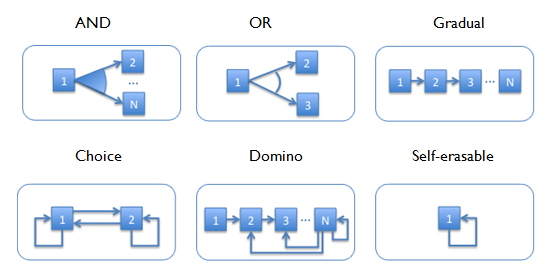
\includegraphics[width=0.95\textwidth]{figs/4-PatronesBlinks.png}
\caption{Patrones de diseño basado en blinks predefinidos en WebMakeUp.}
\label{fig:PatronesBlink}
\end{center}
\end{figure}

En la Figura \ref{fig:PatronesBlink} se observan los diferentes patrones que ahora se comentan en detalle:

\begin{itemize}
\item{Patrón AND: este patrón permite que al interactuar con un widget controlador se muestren/oculten varios widgets de manera simultánea. Para ello el patrón prepara a todos los widgets con el mismo estado inicial, con tal de que estos a medida que se produzcan los blinks, sigan compartiendo el mismo estado (todos mostrándose o todos ocultos).
 
Es útil cuando se quiere mostrar u ocultar varios widgets simultáneamente.}
\item{Patrón OR: este patrón tiene sentido con 3 widgets, un controlador y 2 observadores. En este caso en cada blink, uno de los observadores se mostrará (el que estuviera oculto) y el otro se ocultará (el que estuviera mostrándose). El funcionamiento es igual que el del AND, con la única diferencia de que el estado inicial no es el mismo en todos los widgets.

Es útil cuando se quiere alternar el contenido que se está mostrando.}
\item{Patrón Gradual: el funcionamiento consiste en indicar varios widgets, donde cada uno al interactuar con él muestra más contenido.

Es útil cuando existe contenido con jerarquía o de árbol, es decir, cuando hay contenido que depende de otro contenido para tener utilidad en la web.}
\item{Patrón Choice: permite alternar entre dos widgets, si se muestra uno el otro estará oculto y viceversa. El intercambio se produce realizando una interacción sobre él mismo.

Esto es útil cuando se quiere ir alternando entre diferente contenido sin necesidad de otro widget.}
\item{Patrón Domino: el funcionamiento es similar al de un dominó, donde al interaccionar con un widget muestra el siguiente y así sucesivamente. Cuando se interacciona con el último este oculta todos los anteriores (exceptuando el primero, para que pueda volver a producirse el efecto dominó).

Esto es útil en información de tipo jerárquica.}
\item{Patrón Self-erasable: al interactuar con él se oculta, no volviendo a mostrarse nunca más hasta que se vuelva a visitar el sitio web.

Esto es útil en caso de información que se quiere leer una vez y no más. Un ejemplo ya implementado en los sitios web por ley actualmente, son los widgets con la advertencia de uso Cookies de terceros.}
\end{itemize}

El uso de estos patrones permite generar dinamismo a los sitios web de manera muy ágil y sencilla.

La razón de utilizarlo de esa manera surge de los SmartArt de Microsoft PowerPoint. Los SmartArt son elementos gráficos que permiten generar diferentes patrones de disposición de los datos, de forma piramidal, jerárquica, cíclica, etc.

En SmartArt, simplemente hay que seleccionar qué datos se toman en cuenta y se elige un patrón. De manera automática, genera un gráfico con la representación de esos datos. En la Figura \ref{fig:SmartArt} se muestra cómo la estructura de datos se convierte en un gráfico que representa mejor el círculo PDCA\footnote{Ciclo de mejora continua o círculo de Deming: \url{http://en.wikipedia.org/wiki/PDCA}}.

En WebMakeUp el funcionamiento es igual. Se seleccionan los widgets participantes y el patrón que van a seguir. De manera automática se generan los diferentes links entre los widgets participantes cumpliendo con ese patrón.

\begin{figure}
\begin{center}
\subfloat[Estructura por defecto]{
	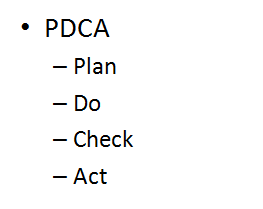
\includegraphics[width=0.45\textwidth]{figs/4-SmartArtDefault.png}
}
\subfloat[Gráfico SmartArt]{
	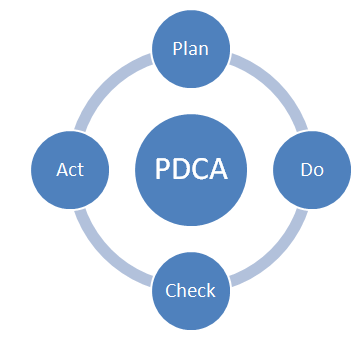
\includegraphics[width=0.45\textwidth]{figs/4-SmartArtGraph.png}
}
\caption{Representación por defecto y gráfica del ciclo PDCA mediante SmartArt de PowerPoint.}
\label{fig:SmartArt}
\end{center}
\end{figure}

Estos patrones no se desarrollaron en este PFG, pero sirven para validar el generador de extensiones. Estos patrones tienen que ser capaces de funcionar en tiempo de ejecución de la aumentación (Apartado \ref{sec:ValidacionGenerador}).

Para finalizar con este capítulo, cabe destacar que al estar aún en pleno desarrollo WebMakeUp, todavía quedaría por realizar una prueba con usuarios reales para ver cómo se adaptarían a estos nuevos cambios. Aunque tal y como se ha ido observando en el trabajo con los blinks la realización de aumentaciones con interacciones es más rápida, y se confía en la buena aceptación del público en general.
\chapter{Creación de extensiones Chrome a partir del modelo de aumentación}
\label{cha:generador}
\chaptermark{Transformador de extensiones}

En este capítulo se tratan diferentes temas relacionados con la generación de la aumentación para implantarla en el navegador.

Para ubicarse, en primer lugar se realiza una aumentación web con el editor WebMakeUp. Posteriormente, se genera una extensión de Google Chrome. Esta se instala y se ejecuta en el sitio web que se indique en tiempo de edición para mostrar la aumentación que se desea.

Por lo tanto, este capítulo va dedicado a explicar cómo se crea la extensión de Google Chrome a partir del modelo de datos que proporciona en tiempo de edición la herramienta WebMakeUp. En primer lugar, se habla del modelo de aumentación del editor, que es independiente de la plataforma en la que se va a generar (Platform Independent Model, a partir de ahora PIM) en el Apartado \ref{sec:PIM}.

Posteriormente, hay que hablar del modelo específico de dominio (Platform Specific Model, a partir de ahora PSM), donde en este PFG se decide crear una extensión de Google Chrome utilizando como base algunas librerías entre la que se destaca ConstraintJS. Para ello, hay que explicar claramente cómo es la plataforma y cómo es el modelo resultante de la transformación.

Asimismo, hay que describir cómo se hace esa transformación y cómo se ejecuta la aumentación (Apartado \ref{sec:DescripcionGenerador}).

Finalmente se muestran algunos ejemplos de aumentación (Apartado \ref{sec:EjemplosGenerador}) y una validación final en base a los patrones y tipos de widgets existentes (Apartado \ref{sec:ValidacionGenerador}).

\section{Platform Independent Model - Modelo independiente de la plataforma}
\label{sec:PIM}

A la hora de crear una extensión, en primer lugar hay que explicar cuál es el proceso. En el editor WebMakeUp, la aumentación se refleja de manera gráfica para el usuario. Además existe un modelo asociado a la aumentación, que es el que se encarga de representarla internamente.

Esta representación interna puede servir para 2 aspectos en prácticamente cualquier editor del mercado:
\begin{itemize}
\item{Permitir dar persistencia en el trabajo que se está realizando, lo que habitualmente se denomina guardar. Asociado con el concepto de guardar un proyecto del editor, existe la opción inversa, que es cargar un proyecto en el editor. Para permitir esto, hay que representar en un modelo de datos el trabajo que se está realizando.}
\item{Permitir exportar los resultados del trabajo, generando un resultado, que al final es el que se va a utilizar. Para ello también se utiliza un modelo de datos.}
\end{itemize}

Este PFG se ha centrado en una pequeña parte de exportar un resultado final, todo ello a partir del modelo de datos que proporciona WebMakeUp. El trabajo realizado es el empaquetamiento de la extensión y el modelo de interacción (ver Capítulo \ref{cha:interacciones}). Asimismo, en WebMakeUp pero fuera del PFG se trabaja con la creación en tiempo de ejecución de los widgets y el posicionamiento del mismo. Sobre esto último también hay que comentar algunos aspectos, dado que pertenece todo al transformador.

En la Figura \ref{fig:MetamodeloWebMakeUp} se muestra todo el metamodelo de WebMakeUp. En el se representan todos los aspectos de la aumentación: propiedades de los widgets (la clase Widget y sus relaciones), propiedades de interacción (representado mediante Blinks), y de la propia aumentación (la clase Mod).

\begin{figure}
\begin{center}
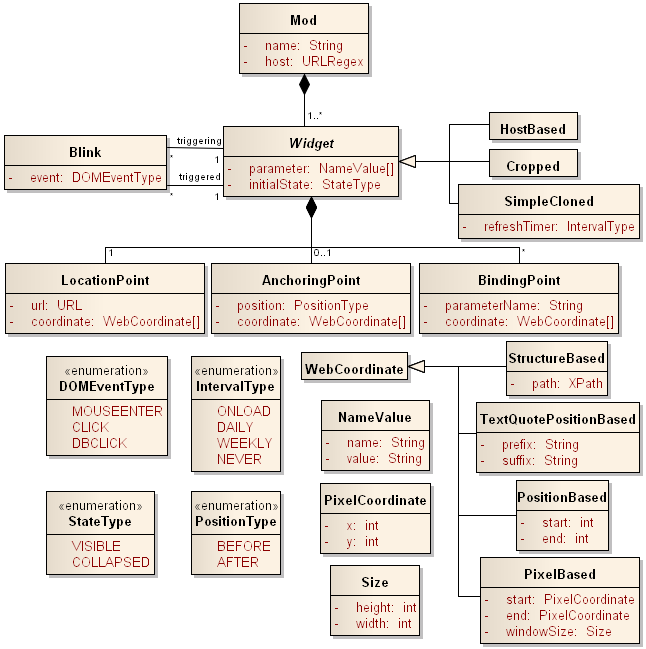
\includegraphics[width=0.65\textwidth]{figs/5-MetamodeloWebMakeUp.png}
\caption{Metamodelo de WebMakeUp que representa cómo es una aumentación web.}
\label{fig:MetamodeloWebMakeUp}
\end{center}
\end{figure}

Este PFG se centra únicamente en las clases del metamodelo que representan las configuraciones de la extensión (la clase \textbf{Mod}) y en cómo generar un código que sea capaz de plasmar las interacciones (la relación entre \textbf{Widgets} mediante \textbf{Blinks}). Estas clases del metamodelo se pueden ver en la Figura \ref{fig:MetamodeloWebMakeUpReducido}. 

Asimismo, hay widgets que acceden a recursos fuera del sitio web donde se ejecuta la aumentación. Esto requiere de permisos adicionales, dado que por defecto una aumentación sólo puede acceder al sitio web donde se ejecuta. Por lo tanto, la clase \textbf{LocationPoint} almacena las URLs externas a las que tiene acceso un Widget. Con ello se consigue en tiempo de transformación indicar a la extensión de Google Chrome los permisos estrictamente necesarios, ofreciendo mayor seguridad a las aumentaciones creadas.

\begin{figure}
\begin{center}
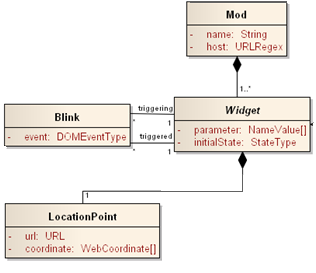
\includegraphics[width=0.45\textwidth]{figs/5-MetamodeloWebMakeUpReducido.png}
\caption{Parte del metamodelo de WebMakeUp del que se extrae la información de la aumentación y las animaciones.}
\label{fig:MetamodeloWebMakeUpReducido}
\end{center}
\end{figure}


\section{Platform Specific Model - Modelo especifico de la plataforma}
\label{sec:PSM}

En este apartado se trata de definir cómo es la plataforma sobre la que va a ejecutarse la aumentación. Es necesario conocer cómo es la plataforma para poder generar un artefacto acorde a las especificaciones que se detallan en la propia plataforma.

Cómo se ha ido comentando a lo largo de este documento, la plataforma sobre la que se ha trabajado ha sido Google Chrome. WebMakeUp está desarrollado sobre Google Chrome y las aumentaciones que crea son específicamente para Google Chrome. Por tanto, se debe hablar de cómo es Google Chrome (Apartado \ref{sec:PSM-GoogleChrome}).

\subsection{Google Chrome}
\label{sec:PSM-GoogleChrome}
Google Chrome es un navegador Web de uso general. El navegador ha sido desarrollado a partir del proyecto Chromium\footnote{Web del proyecto Chromium: \url{http://www.chromium.org/}}, pero el navegador que este proyecto ofrece no está apoyado ni comercial ni técnicamente por Google.

En este PFG, el uso de Google Chrome fue impuesto, por tanto no se tuvo que realizar ningún tipo de estudio sobre qué plataforma utilizar para el desarrollo de WebMakeUp, ni tampoco de las aumentaciones que se crean. Aun así, es necesario mencionar el porqué Google Chrome en lugar de otros. 

Existe una razón principal, que es el uso de Google Chrome en el mercado. Google Chrome se lanza al mercado de manera oficial en septiembre de 2008. Como se muestra en la Figura \ref{fig:UsoGoogleChrome} a mediados de 2012 ya consigue desbancar a Internet Explorer como navegador más utilizado. Actualmente presenta una cuota de un 45\% de uso en el mercado, tanto en PC, como en otros dispositivos.

\begin{figure}
\begin{center}
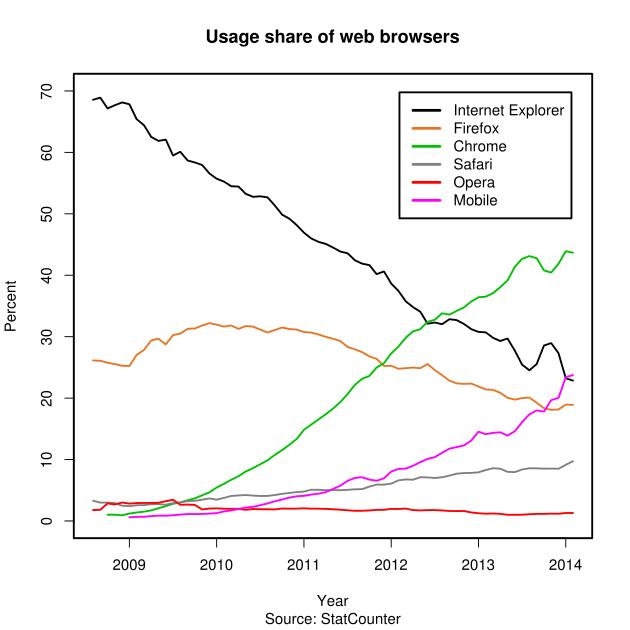
\includegraphics[width=0.65\textwidth]{figs/5-UsoGoogleChrome.png}
\caption{Utilización de Google Chrome en el mercado.}
\label{fig:UsoGoogleChrome}
\end{center}
\end{figure}

En este caso, únicamente hay que comentar cómo es Google Chrome para PC, ya sea en sus versiones para Windows, MacOS o Linux, que presentan una interfaz prácticamente idéntica (no únicamente gráfica, sino también de desarrollo).

Google Chrome, al igual que otros navegadores actuales ofrecen posibilidades de extensión de las funcionalidades que ofrecen. Esta extensibilidad del navegador en Google Chrome se pueden hacer de 2 formas. Por un lado existen las \emph{apps} y por otro lado las extensiones.

Las Google Chrome apps\footnote{Google Chrome apps:\url{https://support.google.com/chrome/answer/1050586?hl=en}} en realidad son aplicaciones puramente del lado servidor. Google Chrome permite la instalación de estas apps y con ello tener un acceso directo desde el navegador o incluso desde el propio sistema operativo.

En este caso al trabajar con aumentación web esta opción no es interesante, dado que se requiere de un lado servidor del que no se va a disponer. Por tanto, existen las extensiones, que permiten modificar las funcionalidades y tareas que realiza el navegador de manera local. Es decir, la extensión se ejecuta en el lado cliente y no repercute en el lado servidor.

Existen 2 maneras de desarrollar extensiones en Google Chrome, mediante el uso de \emph{userscripts} o mediante extensiones nativas de Google Chrome.

Un \emph{userscript}\footnote{Ejemplos de userscript:  \url{http://userscripts.org:8080/}} está constituido por un fichero, que es un \emph{script}, programado en Javascript. Este brinda la posibilidad de hacer modificaciones en el DOM del sitio web y aplicar algunas cláusulas de permisos, y de recursos utilizados. Estos \emph{userscript} pueden ser utilizados en cualquier navegador que sea capaz de interpretarlos. Actualmente tanto Firefox como Google Chrome son capaces de interpretarlos de manera nativa.

Inspirado en los \emph{userscript}, Google Chrome dispone de extensiones nativas. Con inspirado se quiere decir que el creador de los \emph{userscript}, también participó en el desarrollo de la extensiones de Google Chrome y que la especificación de algunas cosas son similares. La principal diferencia es que una extensión de Google Chrome permite no solo el acceso al DOM, si no a múltiples características del propio navegador (como la persistencia de datos). En el caso del editor de mods WebMakeUp, se pueden almacenar aumentaciones sin exportar y recuperarlas para seguir editando en otro momento. Para ello utiliza la persistencia que ofrece Google Chrome en su API\footnote{Persistencia en Google Chrome mediante HTML5 y javascript: \url{http://mysticalpotato.wordpress.com/2011/01/23/html5-y-json-para-dotar-de-persistencia-a-una-extension-de-chrome/}}.

Las extensiones nativas de Google Chrome se pueden instalar de 2 maneras.

Por un lado, existe el Chrome Store\footnote{Sitio web del Chrome Store: \url{https://chrome.google.com/webstore}}, que es una tienda online que permite instalar apps y extensiones nativas en un clic, mantiene la sincronización entre los diferentes PCs con Chrome donde se tenga la cuenta de Google iniciada. El fichero que se instala es un contenedor firmado por el creador de la extensión y que garantiza la integridad del mismo ofreciendo seguridad.

Por otro lado, existe la posibilidad de instalarla desde el PC, desde una carpeta que cumpla con las especificaciones de una extensión de Google Chrome que se explica a continuación. Dado que en este PFG no se abarca la posibilidad de publicación de la extensión que el usuario crea con el editor WebMakeUp, lo que se crea es un comprimido .zip con el código necesario para implantar y ejecutar la aumentación en el navegador.

Las extensiones de Google Chrome son sencillas de programar. Para ello Google Chrome interpreta los 3 lenguajes del lado cliente que se utilizan en el desarrollo del lado cliente de la web, HTML, CSS y Javascript. En las extensiones nativas, al igual que en los \emph{userscripts} predomina Javascript, dado que el contenido de la web ya existe (se obtiene de un sitio web). Muchas veces los estilos también se mantienen dado que las extensiones habitualmente cambian la funcionalidad y pocas veces en el estilo. Por tanto, los mayores cambios se van a notar en el comportamiento del sitio y eso corresponde a Javascript.

En Google Chrome existen diferentes áreas de trabajo. La estructura de una extensión divide las zonas de acción de la extensión. Tal y cómo se muestra en la Figura \ref{fig:arquitecturaChrome}, existe un fichero principal, llamado \emph{manifest.json}.

\begin{figure}
\begin{center}
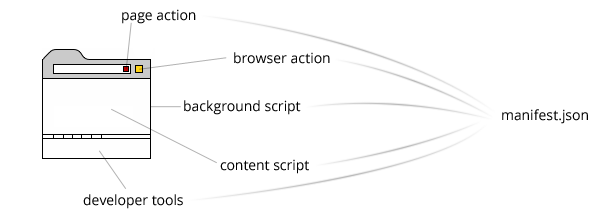
\includegraphics[width=0.75\textwidth]{figs/5-chromeArchitecture.png}
\caption{Arquitectura de desarrollo de Google Chrome donde se observa en qué parte actúa cada área de la extensión.}
\label{fig:arquitecturaChrome}
\end{center}
\end{figure}

El manifest.json es el único fichero en una extensión de Google Chrome que es obligatorio. En la Figura \ref{fig:chromeManifest} se observa un fichero básico manifest.json que ayudará a explicar la estructura que se necesita para desarrollar una extensión.

\begin{figure}
\begin{center}
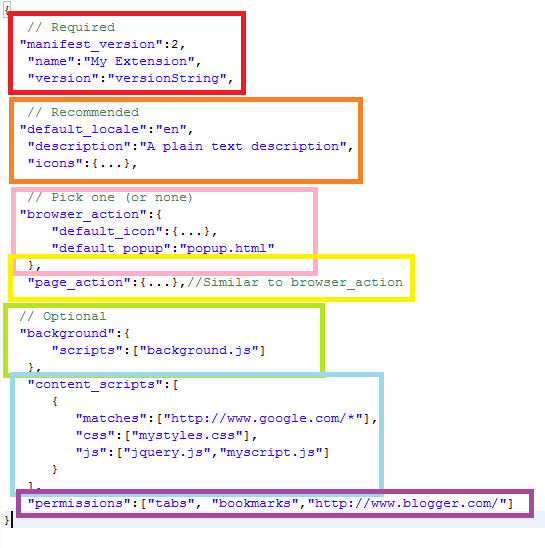
\includegraphics[width=0.65\textwidth]{figs/5-Manifest.png}
\caption{Estructura básica del fichero de manifest.}
\label{fig:chromeManifest}
\end{center}
\end{figure}

Por un lado, se gestionan las propiedades generales (en negrita se marcan las obligatorias):
\begin{itemize}
\item{\textbf{Versión del manifiesto}: actualmente se utiliza la v2. En los \emph{userscript}, que también tienen su propio manifiesto, se utilizaba la v1, aunque ya está obsoleta.}
\item{\textbf{Nombre}: nombre de la extensión.}
\item{\textbf{Versión}: versión en la que se encuentra la extensión creada.}
\item{Descripción: descripción de la extensión. Se suele utilizar para describir para qué sirve la extensión o dónde se utiliza.}
\item{Permisos: a qué recursos puede acceder la extensión. Qué sitios web, si utiliza persistencia para almacenar los datos, etc.}
\end{itemize}

Por otro lado, se definen los ficheros que conforman las diferentes áreas de trabajo que se muestran en la Figura \ref{fig:arquitecturaChrome}:
\begin{itemize}
\item{Page action: su uso común es el de notificar dentro de la barra de dirección/búsqueda de Chrome.}
\item{Browser action: proporciona un menú para la extensión. Por ejemplo en WebMakeUp ahí está el menú para iniciar el editor, guardar, cargar y exportar la aumentación.}
\item{Background script: cada extensión crea un nuevo proceso de Google Chrome en el sistema operativo. Cada pestaña también tiene su propio proceso. El background es código que se ejecuta en el proceso de la extensión y lo comparten todas las pestañas. Dispone de algunos permisos cómo acceso a componentes del navegador, por ejemplo, para poder almacenar datos.}
\item{Content script: lo conforman los scripts que se ejecutan en una pestaña concreta. Se le pueden indicar en qué sitios webs tiene que actuar. En la Figura \ref{fig:chromeManifest} de color azul se observa en matches que actuará solo en el sitio de \url{www.google.com} y que se interpretarán dos Javascripts y un fichero de CSS. Dispone de acceso al DOM, pero no puede acceder a componentes del navegador.}
\end{itemize}

Una aumentación el único fin que tiene es modificar el DOM, que es donde se trabaja con los widgets que están dispuestos en él. Por tanto, lo razonable es que la aumentación que se va a generar trabaje sobre el content script.

En el Apartado \ref{sec:DescripcionGenerador} se habla sobre como funciona el transformador de la extensión en base al modelo de datos que proporciona WebMakeUp (Apartado \ref{sec:PIM}) y junto a la plataforma especifica (Google Chrome) que se ha descrito en este apartado.

\section{Descripción de la transformación de la extensión}
\label{sec:DescripcionGenerador}

Antes de comenzar a explicar cómo se obtiene la transformación de la extensión, hay que tener claro un concepto relacionado con Javascript. Tal y como se ha ido mencionando en apartados anteriores, Javascript es un lenguaje interpretado.

El lenguaje de programación C es un lenguaje que se compila obteniendo un código ejecutable por la máquina. Este código, posteriormente se ejecuta en una máquina que cumpla con las mismas características (como la arquitectura de la CPU).

En Javascript, el código fuente no se compila. Existe un intérprete (llamado motor Javascript) que es capaz en tiempo de ejecución de interpretar ese código y ejecutarlo. Cada navegador tiene su propio intérprete y no todos interpretan las instrucciones de la misma manera. Para ello, existen estándares como \emph{ECMAScript} que permiten garantizar que esa interpretación será idéntica en los diferentes intérpretes existentes en el mercado.

¿Qué ventajas ofrece que sea interpretado? Permite que el mismo fichero .js sea multiplataforma. Esto es lógico hacerlo dado que Javascript es un lenguaje de uso en Internet, donde los usuarios disponen de diferentes plataformas y acceden al mismo contenido.

Una vez aclarado cómo funciona Javascript, hay que dividir la transformación de la extensión en dos fases. Por un lado, la generación/creación de la extensión de Google Chrome, y por otro lado, la ejecución de la misma.

\subsection{Creación de la extensión de Chrome}
\label{sec:CreacionExtension}

En este apartado el objetivo es sencillo. Hay que realizar una traducción del lenguaje que conoce WebMakeUp (el modelo de datos de la aumentación) al lenguaje que conoce Google Chrome (la arquitectura de extensión nativa de Google Chrome).

Dado que se ha decidido interpretar el modelo en tiempo de ejecución (ver Apartado \ref{sec:EjecucionExtension}), en la creación de la extensión simplemente hay que generar el manifest.json y el modelo de datos que posteriormente se interpreta.

El manifest.json tiene una parte que es común a todas las extensiones que se generan y una parte dinámica dependiendo de la aumentación. En la Figura \ref{fig:generatedManifestStaticDynamic} se diferencian los campos comunes a todas las extensiones (versión, estilos y Javascripts a ejecutar en el context script), y las variables dependiendo de la aumentación que se cree (nombre, descripción, sitios webs donde se ejecuta y permisos).

\begin{figure}
\begin{center}
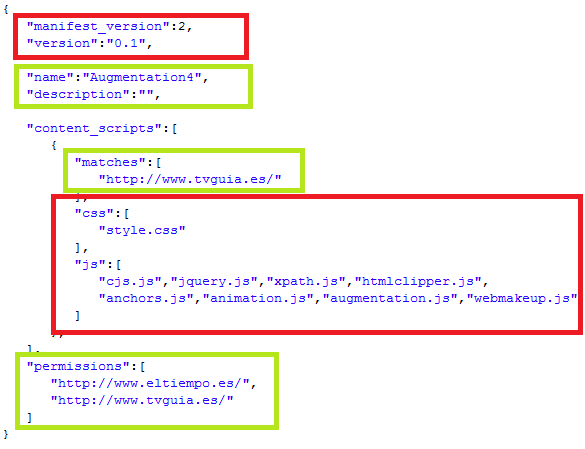
\includegraphics[width=0.65\textwidth]{figs/5-generatedManifestStaticDynamic.png}
\caption{Fichero manifest.json donde se diferencia la parte común (rojo) a todas las extensiones de la parte variable (verde).}
\label{fig:generatedManifestStaticDynamic}
\end{center}
\end{figure}

Estos datos se obtienen del modelo, en este caso de las clases que se presentan en la Figura \ref{fig:MetamodelReducedManifest}.

\begin{figure}
\centering
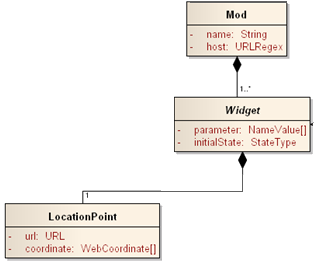
\includegraphics[width=0.5\textwidth]{./figs/5-MetamodelReducedManifest}
\caption{Parte del metamodelo que se utiliza en tiempo de generación de la extensión.}
\label{fig:MetamodelReducedManifest}
\end{figure}


Un \emph{Mod} tiene un nombre, una descripción y una \emph{URLRegex}, que es una expresión regular que indica el sitio/sitios donde se va a ejecutar.

A su vez, dependiendo de los widgets, estos pueden ser de diferentes tipos. Si estos requieren obtener algún tipo de datos de otro sitio web se tiene que proporcionar permisos para ello. Cada widget dispone de un location point con la URL a la que accede y en este caso lo que se hace es añadirla a los sitios permitidos.

Además del manifest, hay que importar el modelo de WebMakeUp para que se interprete en tiempo de ejecución. Para ello se realiza una conversión del objeto JSON que contiene todo el modelo de datos de WebMakeUp a \emph{string} gracias a la función \emph{JSON.stringify()} de Javascript.

Finalmente, se empaquetan todas las librerías necesarias para su futura interpretación en \emph{runtime} (tiempo de ejecución), para presentarle al usuario un fichero .zip comprimido con la extensión generada. Para empaquetar la extensión se utiliza una librería llamada JSzip \footnote{Web oficial de jszip: \url{http://stuk.github.io/jszip/}}. En ella se convierten los \emph{strings} en ficheros incluidos en un objeto \emph{BLOB} (Objeto Binario Largo) que actúa de contenedor. Para presentarle este objeto al usuario, se ha utilizado la librería FileSaver\footnote{Sitio web oficial de FileSaver: \url{https://github.com/eligrey/FileSaver.js/}}. Con ella se hace una descarga del BLOB, que en este caso es un fichero contenedor en .zip.

El resultado final es el que se presenta en la Figura \ref{fig:ExtensionEmpaquetada}. En él se incluye el fichero manifest.json que se ha generado y el fichero webmakeup.js que incluye el modelo de datos en formato JSON. El resto de ficheros sirven para interpretar el modelo y poder ejecutar la aumentación en \emph{runtime}.

\begin{figure}
\centering
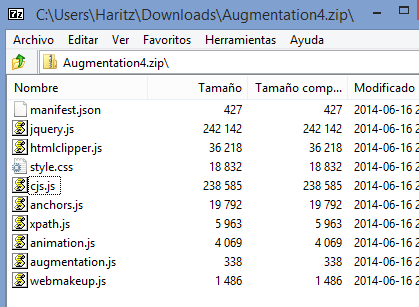
\includegraphics[width=0.7\linewidth]{./figs/5-ExtensionEmpaquetada}
\caption{Extensión empaquetada que se genera a partir de la aumentación}
\label{fig:ExtensionEmpaquetada}
\end{figure}


\subsection{Ejecución de la extensión}
\label{sec:EjecucionExtension}

Una vez generada la extensión (Apartado \ref{sec:CreacionExtension}), en este apartado se habla de cómo se interpreta el modelo de datos para crear la aumentación.

Tal y como se ha comentado previamente, el código puede ser compilado o interpretado. Incluso en el propio WebMakeUp en tiempo de generación se puede haber compilado (o creado) las instrucciones Javascript que se van a ejecutar. Como prueba de ello, en la primera versión de WebMakeUp basada en diagramas de transición de estados se generaban las instrucciones Javascript. En la Figura \ref{fig:generatedCompiledCodeSTD} se muestra que los datos están en el propio código. Se reflejan los estados que se crean y las transiciones existentes, donde los parámetros de las funciones a las que se llaman están estos datos sin ofrecer ninguna estructura.

\begin{figure}
\centering
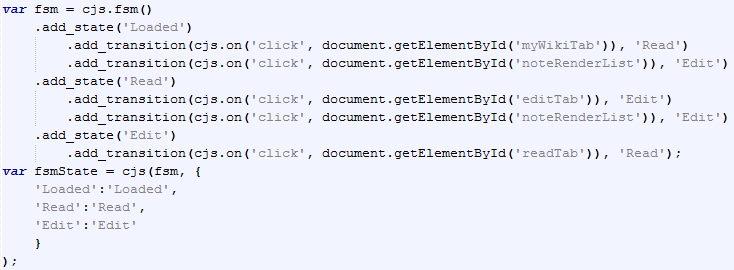
\includegraphics[width=0.95\linewidth]{./figs/5-generatedCompiledCodeSTD}
\caption{Código pre-compilado con la máquina de transición de estados que se crea en tiempo de ejecución.}
\label{fig:generatedCompiledCodeSTD}
\end{figure}

El realizarlo de esta manera no supone ninguna ventaja práctica, dado que la ventaja principal del código compilado es que se ejecuta más rápido, pero Javascript es interpretado. Por tanto interpretar un código que interpreta un modelo de datos en coste es prácticamente idéntico a un código con las funciones a ejecutar ya preparadas para ser interpretadas.

Las ventajas de generar únicamente un modelo e interpretarlo en tiempo de ejecución, sin embargo, son notorias:
\begin{itemize}
\item{Es más fácil de validar un modelo de datos que la sintaxis y semántica de un lenguaje de programación. Existen herramientas como JSON Schema con el que se pueden validar modelos de datos en JSON, además su coste es pequeño.}
\item{Permite evitar dependencia entre datos y código a ejecutar. Por ejemplo, se puede mantener el mismo modelo de datos y cambiar únicamente el intérprete del modelo. Modificarlo es sencillo, mientras que cambiar el generador de instrucciones Javascript es complejo.}
\item{Es más sencillo hacer re-ingeniería. Al estar independizada la parte del modelo de la interpretación es más sencillo reestructurar los procesos, realizar refactorización, etc.}
\end{itemize}

Tras aclarar el porqué se ha realizado un código que interpreta un modelo, sólo queda por describir cómo se interpreta.

Cabe destacar que del modelo hay que interpretar tanto los widgets como las animaciones. El intérprete de widgets no es parte del PFG, por tanto, simplemente hay que mencionar que su objetivo es crear y posicionar los widgets en el DOM. El intérprete de animaciones si es parte del PFG y es en el que se centra este apartado.

\begin{figure}
\centering
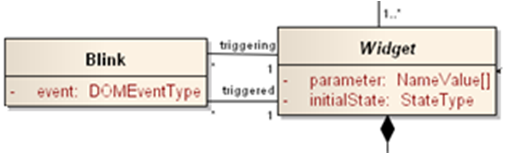
\includegraphics[width=0.7\linewidth]{./figs/5-MetamodelReducedWidgetsBlinks}
\caption{Modelo de datos que describe los blinks de interacción entre widgets}
\label{fig:MetamodelReducedWidgetsBlinks}
\end{figure}

En la Figura \ref{fig:MetamodelReducedWidgetsBlinks} se observan las clases del metamodelo que describen las interacciones basadas en blinks. Como se describe en el Apartado \ref{sec:modeloBlinks}, el blink consta de 2 widgets, un observador (\emph{triggered}) y un controlador (\emph{triggering}), y de un evento que se produce en el \emph{triggering}.

La idea que se ha tenido para representar estas interacciones ha sido mediante STD (diagramas de transición de estados), que en lo que a código se traducen como máquinas de estado finitas (a partir de ahora FSM). Existen dos razones principales para ello:
\begin{itemize}
\item{La previa utilización de FSMs para trabajar con el concepto de estado global de la aumentación en el modelo de interacción basado en STD (Apartado \ref{sec:modeloSTD}).}
\item{La facilidad de representar el concepto de estado de un widget con la misma herramienta que se representaba el estado global (ConstraintJS, descrito en el Anexo \ref{sec:CJS}). Además, la manera de gestionar los manejadores para los diferentes eventos es muy sencilla.}
\end{itemize}

Teniendo en cuenta esto, lo que se genera es una FSM por cada uno de los widgets que tiene al menos un blink en el que participa como observador (\emph{triggered}). Es lógico, dado que ese widget cambiará de estado (de mostrarse a ocultarse y viceversa). Sobre otros widgets (o sobre sí mismo) se pueden producir eventos. Cada vez que se produce un evento sobre un controlador (\emph{triggering}) el observador cambiará de estado. 

En la Figura \ref{fig:blink2WidgetsExample} se muestra un ejemplo que sirve para explicar el cómo se describen las máquinas de estado. En él se presentan tres widgets. Lo que se busca es focalizarse únicamente en el texto superior. Para ello en caso de que se tenga el cursor en el texto superior (Widget 2) las noticias se ocultan (Widget 3). Pero también se puede ocultar el Widget 3 utilizando el widget central (Widget 1) si se hace clic sobre él.

\begin{figure}
\centering
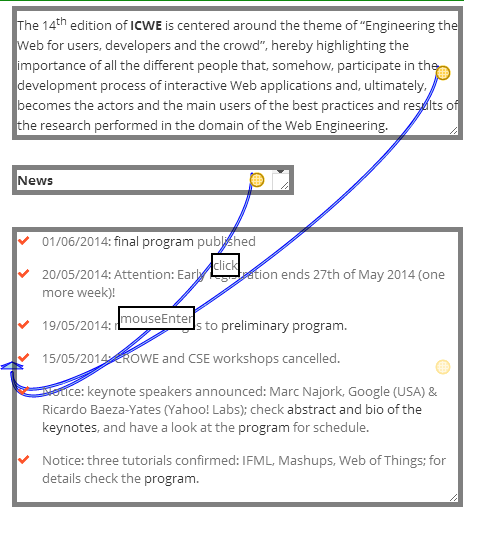
\includegraphics[width=0.5\linewidth]{./figs/5-blink2WidgetsExample}
\caption{Ejemplo de 2 blinks donde el observer es el mismo}
\label{fig:blink2WidgetsExample}
\end{figure}

En la Figura \ref{fig:WidgetFSM} se muestra un cómo se representa en FSM el ejemplo anterior. El widget triggered tiene como estado inicial enable. Existe un blink entre triggered y Widget1 (triggering) con el evento click. Esto significa según el funcionamiento de los blinks, que con el evento click cambia de collapse a enable y con su inverso (el click) vuelve a collapse. Asimismo con el Widget 2 existe un evento que hace que se oculte (mouseover) y otro que con el que vuelve a mostrarse (mouseout).

\begin{figure}
\centering
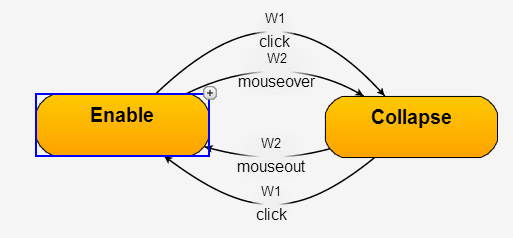
\includegraphics[width=0.7\linewidth]{./figs/5-WidgetFSM}
\caption{Representación en FSM de los estados y transiciones sobre un widget.}
\label{fig:WidgetFSM}
\end{figure}

Por tanto, el intérprete basándose en el modelo de datos debe realizar dos tareas. Por un lado, identificar todos los widgets que participan como triggered en algún blink. Por otro lado, generar para cada uno de esos widgets una FSM con sus eventos y los widgets triggering que participan respectivamente.

Para el primer paso se ha de hacer un recorrido por todos los blinks e ir almacenando por cada widget triggered una lista con los blinks (par evento+triggeringWidget). En la Figura \ref{fig:TriggeredWidgetsJavascript} se puede observar el algoritmo.

\begin{figure}
\centering
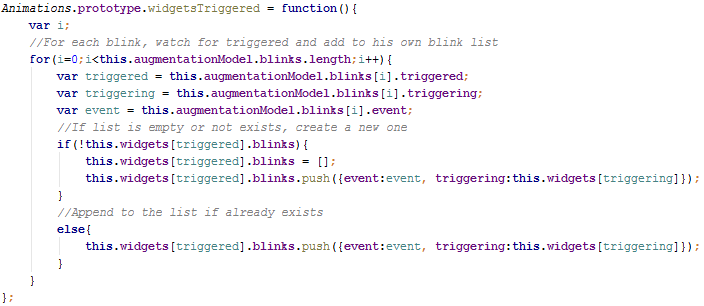
\includegraphics[width=0.7\linewidth]{./figs/5-TriggeredWidgetsJavascript}
\caption{Obtención de los widgets con algún blink en el que tiene la función de observador (triggered).}
\label{fig:TriggeredWidgetsJavascript}
\end{figure}

Para el segundo paso, una vez se obtiene la lista de widgets triggered, utilizando la API de ConstraintJS se crea una FSM para cada widget. La creación como se observa en la Figura \ref{fig:CJSFSMCreation} se realiza en 4 pasos:
\begin{itemize}
\item{Crear los estados de la máquina: enable y collapse.}
\item{Crear un par de transiciones (evento y evento inverso) por cada blink en el que participa como triggered.}
\item{Indicar el estado inicial de la máquina dependiendo del estado inicial del widget.}
\item{Añadir el evento a ejecutar cuando se cambia de estado. De enable->collapse se oculta el widget y de collapse->enable se muestra.}
\end{itemize}

\begin{figure}
\centering
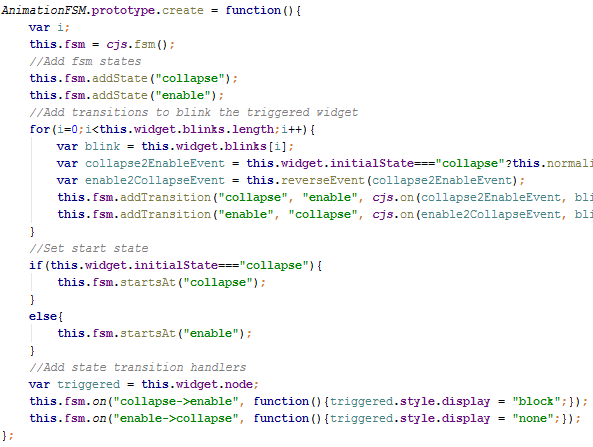
\includegraphics[width=0.7\linewidth]{./figs/5-CJSFSMCreation}
\caption{Creación de la FSM utilizando la API de ConstraintJS}
\label{fig:CJSFSMCreation}
\end{figure}

Una vez creada la FSM, ConstraintJS se encarga de gestionar todos los eventos, las transiciones y los estados de las diferentes máquinas que se crean.

\section{Ejemplos}
\label{sec:EjemplosGenerador}

En este apartado se trata de demostrar el correcto funcionamiento en base a varios ejemplos en diferentes sitios webs y con diferentes tipos de aumentaciones. Estos ejemplos sirven para poder realizar una validación del correcto funcionamiento del transformador (Apartado \ref{sec:ValidacionGenerador}).

El \textbf{ejemplo 1} trata de encaminar los diferentes pasos que hay que realizar para enviar una respuesta a una pregunta en el foro \url{www.stackoverflow.com}. En la Figura \ref{fig:StackOverflowDefault} se observa un formulario en tres pasos. Paso 1, responder la pregunta que se ha hecho. Paso 2, se indican los datos de usuario. Paso 3, se envía la respuesta aceptando los términos de acuerdo. En la Figura \ref{fig:StackOverflowEditor} se muestra que se ha aplicado el patrón zoom-in para ese formulario. Asimismo, abajo hay un widget que muestra un mensaje de si se quiere realizar un tour por StackOverflow. A este widget se le ha aplicado el patrón self-erasable, que una vez leído, si no te interesa el tour se hace clic y elimina el mensaje.

\begin{figure}
\centering
\subfloat[Formulario StackOverflow original]{
	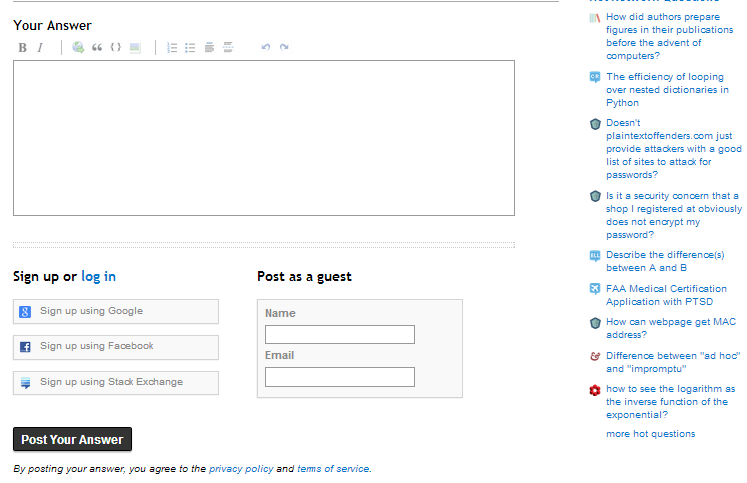
\includegraphics[width=0.5\textwidth]{./figs/5-StackOverflowDefault.png}
	\label{fig:StackOverflowDefault}
}
\subfloat[Editor WebMakeUp aumentando StackOverflow]{
	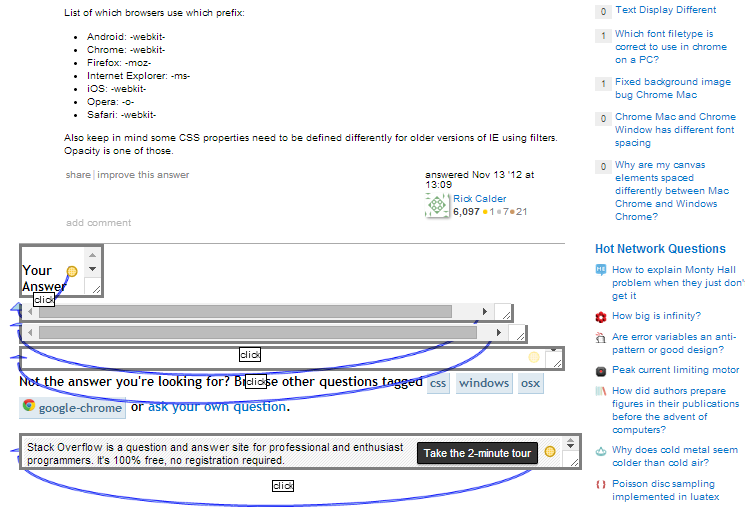
\includegraphics[width=0.5\textwidth]{figs/5-StackOverflow.png}
	\label{fig:StackOverflowEditor}
}
\caption{Ejemplo de aumentación del sitio web StackOverflow.}
\label{fig:StackOverflowExample}
\end{figure}

El \textbf{ejemplo 2} aumenta el sitio \url{http://icwe2013.webengineering.org/program}, que trata sobre el congreso ICWE. En la Figura \ref{fig:ICWEDefault} se muestra en la parte superior izquierda el programa del congreso que se puede o mirar online o descargar. Para aumentarlo, se añade la opción de mostrar u ocultar ambas opciones haciendo clic en el texto Program (Figura \ref{fig:ICWEEditor}). En la inferior izquierda, se muestra el programa para el día 12 de julio. Lo que se ha hecho es utilizando un patrón zoom-in dominó ir mostrando el programa a medida que se va haciendo click en el evento actual, este mostrará el siguiente. Al hacer click en el último evento vuelve a ocultar todos dejándolo compactado. En la parte derecha se ha utilizado un patrón alternate para ir alternando entre los sponsors y los organizadores del ICWE.

\begin{figure}
\centering
\subfloat[Programa del congreso ICWE]{
	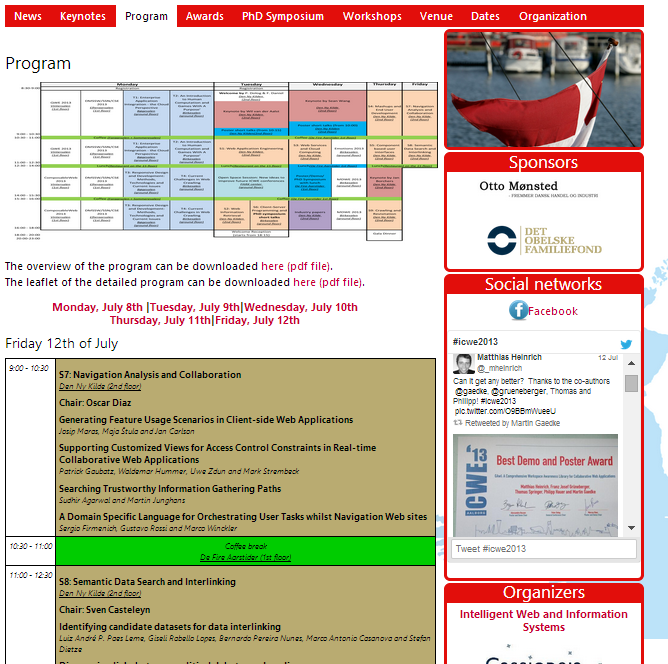
\includegraphics[width=0.5\textwidth]{./figs/5-ICWEDefault.png}
	\label{fig:ICWEDefault}
}
\subfloat[Editor WebMakeUp aumentando ICWE]{
	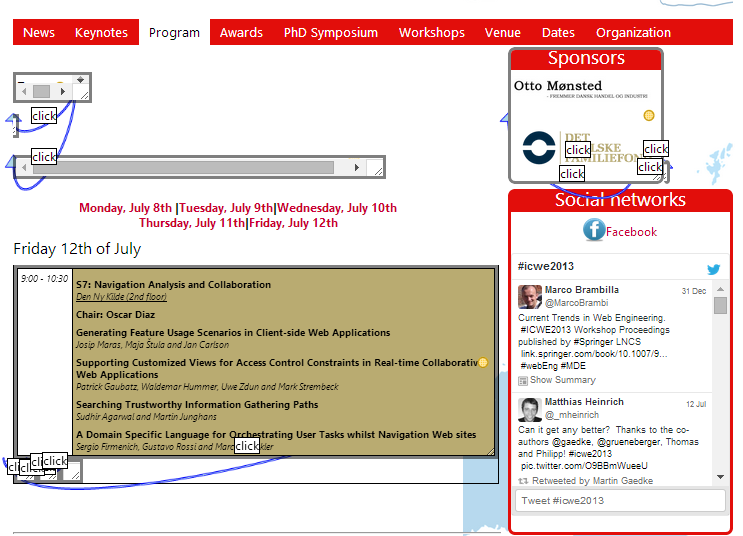
\includegraphics[width=0.5\textwidth]{figs/5-ICWEEditor.png}
	\label{fig:ICWEEditor}
}
\caption{Ejemplo de aumentación del sitio web de ICWE2013.}
\label{fig:ICWEExample}
\end{figure}

En el \textbf{ejemplo 3} se ha aumentado \url{www.tvguia.es} (ver Figura \ref{fig:TVGuiaExample}). En este ejemplo se ha decidido añadir la puntuación de la película de la noche, obtenida de Filmaffinity\footnote{Sitio web del recomendador de cine Filmaffinity: \url{https://www.filmaffinity.com/es/main.html}}, y el gráfico de las puntuaciones. Entre estos dos widgets existe un patrón OR, es decir, o se muestra la puntuación o el gráfico.

\begin{figure}
\centering
\subfloat[Sitio web de tvguia]{
	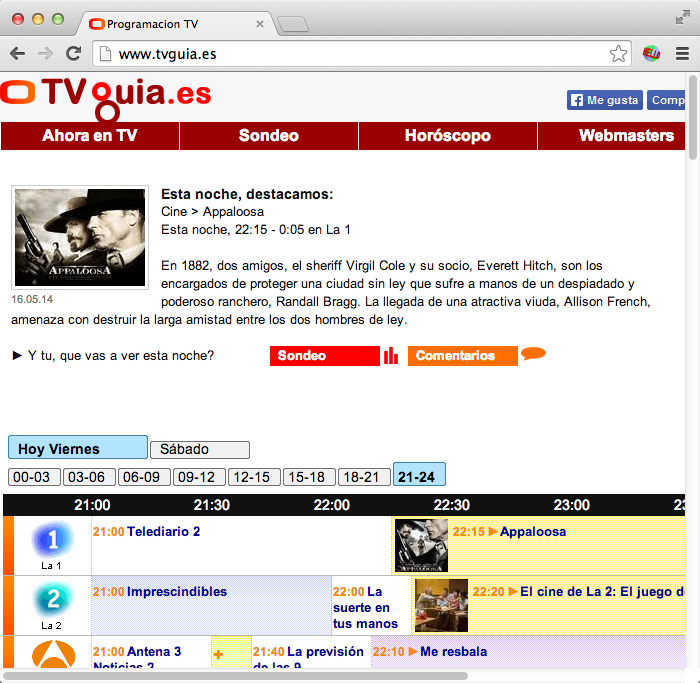
\includegraphics[width=0.5\textwidth]{./figs/5-TVGuiaDefault.png}
	\label{fig:TVGuiaDefault}
}
\subfloat[Editor WebMakeUp aumentando TVGuia]{
	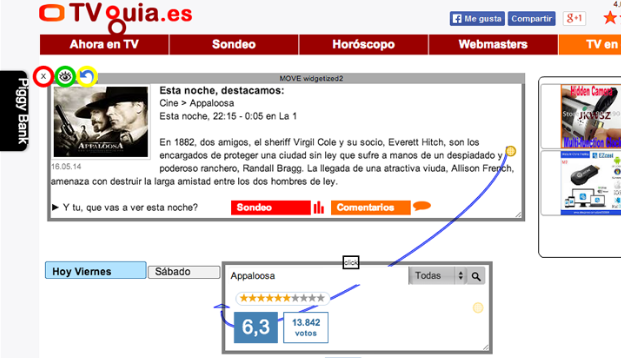
\includegraphics[width=0.5\textwidth]{figs/5-TVGuiaEditor.png}
	\label{fig:TVGuiaEditor}
}
\caption{Ejemplo de aumentación del sitio web de TVGuia.}
\label{fig:TVGuiaExample}
\end{figure}

\section{Validación}
\label{sec:ValidacionGenerador}

En este apartado, tomando como referencia los tres ejemplos que se han mostrado en el Apartado \ref{sec:EjemplosGenerador} se hace una validación de si las pruebas realizadas cubren todos los aspectos que hay que tener en cuenta, y garantizar si el generador realiza bien su trabajo.

Para ello hay que identificar los seis patrones posibles basados en blinks (Apartado \ref{sec:PatronesBlinks}) y los tres tipos de widgets (\textbf{HostBased}, \textbf{Cloned} y \textbf{ComplexCloned}).
\begin{itemize}
\item{HostBased: son los widgets propios de la página web.}
\item{Cloned: son elementos que se extraen de otros sitios webs.}
\item{ComplexCloned: son elementos extraídos de otros sitios webs donde su contenido es complejo. Los ComplexCloned tienen como objetivo, tomando algún elemento del sitio web variable, obtener cierta información remota. En el ejemplo de TVGuia, la película de la noche es variable (cada día hay una diferente). Mediante el buscador de un sitio remoto (en este caso filmaffinity) se puede obtener la puntuación de la película de la noche.}
\end{itemize}

Teniendo en cuenta estos aspectos, en la Tabla \ref{tab:ValidacionGenerador} se muestra qué tipos de widgets y qué patrones abarca cada uno de los ejemplos. Cómo se puede observar, entre los tres ejemplos se validan todos los patrones y los diferentes tipos de widgets, con lo que se puede asegurar que el generador cumple con sus funciones de manera adecuada.

\begin{table}
\centering
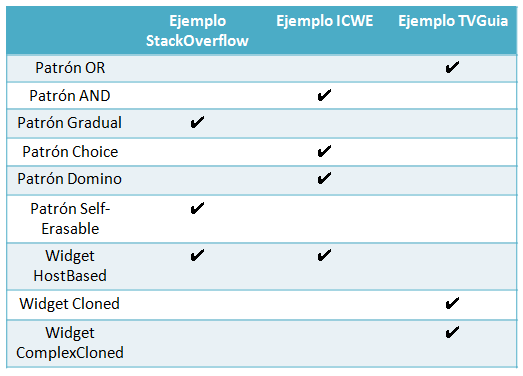
\includegraphics[width=0.7\linewidth]{./figs/5-Validacion.png}
\caption{Tabla de validación de los patrones y tipos de widgets basándose en los ejemplos.}
\label{tab:ValidacionGenerador}
\end{table} 
\chapter{Gestión del Proyecto}
\label{cha:gestion}

\section{Planificación inicial}
\label{sec:Planificacion}

El desarrollo del proyecto transcurre a lo largo del curso académico 2013/2014, donde el inicio del mismo se remonta al 26 de Septiembre de 2013 y la finalización se estima entre el 16 y 18 de Julio de 2014.

Dado el tipo de proyecto, que es un proyecto de innovación con una componente de investigación bastante fuerte, realizar una planificación muy exhaustiva no tiene sentido por dos razones principales:
\begin{enumerate}
\item{La naturaleza del proyecto es incierta. No es un desarrollo convencional donde se tenga definido un objetivo claro y conciso con una especificación muy precisa que pudiera dividirse en tareas muy concretas y realizar una estimación de las mismas.}
\item{El proyecto es de un desarrollo de larga duración, cercano a nueve meses, donde los riesgos e imprevistos son complejos de identificar y un cambio en uno de los periodos iniciales podría trastocar la planificación global continuamente.}
\end{enumerate}

Por estas dos razones principales se decide realizar una planificación más laxa, existiendo colchones de tiempo bastante amplios para las diferentes fases principales del proyecto. Las planificaciones a nivel semanal permite ir adecuando el propio proyecto de manera más efectiva. Además la carga lectiva del alumno era menor dado que sólo tenía que cursar tres asignaturas, una de ellas en el primer cuatrimestre y dos en el segundo. Por lo tanto, se planifica trabajar más en el primero y afrontar una carga menor en el proyecto en el segundo.

Por tanto las fases del proyecto que se definen son las siguientes:
\begin{itemize}
\item{Planificación general: planificación del proyecto, definición de unos objetivos básicos, sin profundizar demasiado en las especificaciones y preparar un entorno de trabajo colaborativo.}
\item{Desarrollo software: incluye estrictamente desarrollo de la aplicación WebMakeUp, donde se trabaja en las diferentes áreas del software como son análisis, diseño, implementación y testing.}
\item{Documentación: tanto la parte de realización de la memoria, cómo el desarrollo de la presentación.}
\end{itemize}
La explicación de que las fases no estén enumeradas es simplemente que hay ciertas fases que se superponen entre si en la franja temporal. Al ser un desarrollo ágil se puede estar trabajando en diferentes fases de manera simultánea y volver a fases anteriores durante el mismo.

\subsection{Estructura de desglose de trabajo - EDT}
\label{sec:EDT}

A continuación se presenta la estructura que desglosa los principales trabajos que se tiene previsto realizar a lo largo del proyecto (Figura \ref{fig:EDT}).

A su vez para conocer en mayor profundidad las principales actividades se adjunta una Tabla \ref{tab:EDT} descriptiva que contiene las principales tareas en las que consiste cada área de trabajo.

\begin{figure}
\begin{center}
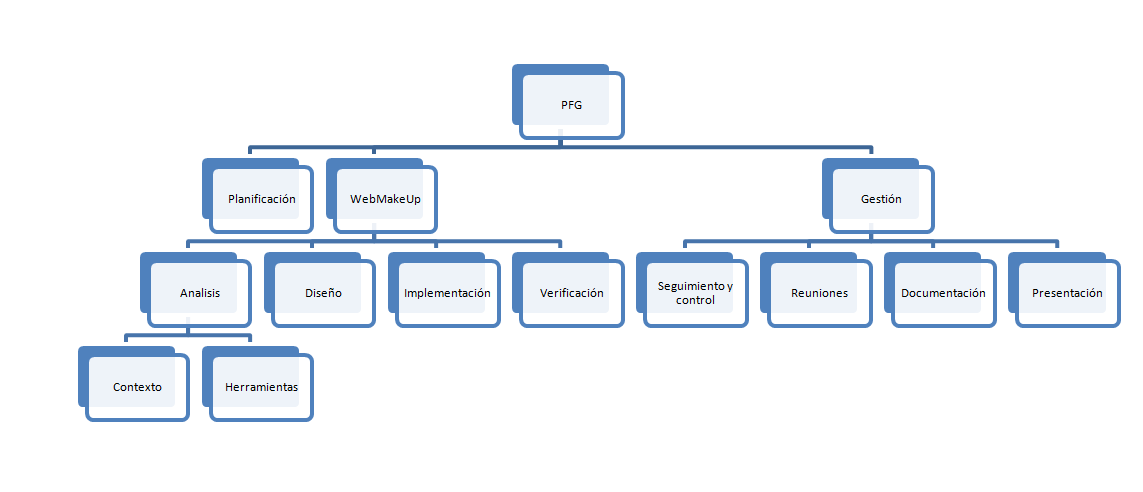
\includegraphics[width=0.95\textwidth]{figs/6-EDT.png}
\caption{Estructura de desglose de trabajo}
\label{fig:EDT}
\end{center}
\end{figure}

\begin{table}
\includegraphics[width=0.95\textwidth]{figs/6-EDTTable.png}
\caption{Descripción de la estructura de trabajo.}
\label{tab:EDT}
\end{table}

\subsection{Diagrama de GANTT e Hitos}
\label{sec:GANTTEHitos}

Dada la naturaleza del proyecto es complejo definir en la línea temporal el cómo se va a desarrollar el proyecto, estimar tiempos o incluso delimitar las fases que hay a lo largo del mismo. Todo va a estar condicionado a medida que se van obteniendo ideas, que modifican continuamente, tanto los objetivos, cómo las herramientas a desarrollar.

Para demostrar la complejidad de definir un diagrama de Hitos, se han dado dos hechos que surgen a lo largo del PFG y que no se prevén en el momento de la planificación:
\begin{itemize}
\item{Durante el mes de enero se decide por parte del grupo de investigación Onekin enviar el proyecto WebMakeUp al congreso ICWE 2014 \footnote{Página web del sitio ICWE 2014: \url{http://icwe2014.webengineering.org/}}. Esto hizo que se tuviera que aumentar el número de horas trabajadas durante el mes de enero.}
\item{Al alumno le sale la oportunidad de hacer prácticas en empresa durante tres meses. Esto hizo que descendiera el número de horas trabajadas frente a las previstas durante los meses de marzo, abril y mayo.}
\end{itemize}

Teniendo en cuenta que pueden suceder cosas de este tipo, se decidió hacer una planificación inicial en base a un desarrollo por iteraciones. Se pretende hacer una primera iteración teniendo en cuenta que se disponía de más tiempo en el primer trimestre con un \emph{Hello World} funcional de la aplicación que se refina reunión tras reunión. Se preparan diferentes prototipos y se van aceptando o descartando los cambios que se van añadiendo a la herramienta. En la segunda iteración, más corta, tras probar la herramienta con usuarios finales, se siguen haciendo mejoras en caso de que fuesen necesarias.

Tal cómo se muestra en la figura \ref{fig:Gantt} se dividen por un lado las dos iteraciones, y también la parte más relacionada con el proyecto y la gestión del PFG. Al haber tantos condicionantes y tantas incógnitas, a pesar de crear una planificación general al inicio, la metodología que se adopta es la de planificaciones semanales y control exhaustivo. Con ello, se ve cómo se modifica el objetivo del proyecto que no está claramente definido desde el inicio.

El no tener un objetivo excesivamente definido, por el tipo de proyecto que es, permite ir adaptándolo a medida que se va haciendo el desarrollo, teniendo un mayor margen de maniobra sobre los objetivos adoptados al inicio. El mayor inconveniente, es que al no tener una planificación demasiado restrictiva, se puede dar el caso de que no se consiguiera el objetivo de concluir con el desarrollo completo.

De igual manera, el desarrollo ágil implica que el desarrollo no se divide en cuatro fases (análisis, diseño, implementación y testing) claramente diferenciadas en la línea temporal. Se va pasando por esas cuatro fases de manera continua. De ahí la razón de que en la Figura \ref{fig:Gantt} las fases del desarrollo se solapen durante toda la iteración.

\begin{figure}
\begin{center}
\includegraphics[width=0.65\textwidth]{figs/6-Gantt.png}
\caption{Diagrama de Gantt}
\label{fig:Gantt}
\end{center}
\end{figure}

\begin{figure}
\begin{center}
\includegraphics[width=0.65\textwidth]{figs/6-Hitos.png}
\caption{Diagrama de Hitos}
\label{fig:Hitos}
\end{center}
\end{figure}

Tal como se observa en el diagrama de la Figura \ref{fig:Hitos} existen cinco hitos que si se han definido desde un principio:

\begin{itemize}
\item{Comienzo del proyecto: 26 de septiembre de 2013. Fecha en la que se da inicio al proyecto y se pre-inscribe en GAUR.}
\item{Final de la primera iteración: finales de febrero.}
\item{Final de la segunda iteración: finales de abril.}
\item{Matriculación del proyecto en GAUR: 23 de junio de 2014 y a su vez entrega en ADDI del proyecto: 1 de julio de 2014 (fecha límite).}
\item{Final del proyecto: 16-18 de julio de 2014. Fecha en la que se presenta el proyecto ante el tribunal.}
\end{itemize}

En base a todas estas premisas, se hace una estimación de tiempo invertido en cada una de las fases del proyecto que se desglosa en la Tabla \ref{tab:TiemposPlanificacion}. Lógicamente esta tabla iba a ser simplemente orientativa, dado que los recursos de los que se dispone en este proyecto eran mayores. El uso de los recursos temporales principalmente depende de cómo se fuese desarrollando el proyecto y cómo se va disponiendo de ellos, dependiendo de la carga de las asignaturas del curso lectivo, que prevalecen en todo momento frente al PFG.

Como se observa en la Tabla \ref{tab:TiemposPlanificacion}, se hace una estimación donde se dedican algo más del 50\% al desarrollo del proyecto y el resto a planificación, seguimiento y documentación. La razón de ello es que al trabajar en grupo y al ser un proyecto de innovación es vital llevar un seguimiento muy exhaustivo. De igual manera, al trabajar con ideas innovadoras, hay que ser bastante meticuloso explicando lo que se ha desarrollado, ya que no es trivial, y por tanto dedicarle muchos recursos y aprovecharlos bien es importante. Por último, los valores añadidos que se quieren realizar con este proyecto requieren de trabajo en estos aspectos que no son puramente de desarrollo.

\begin{table}
\begin{center}
\includegraphics[width=0.95\textwidth]{figs/6-TiemposPlanificacion.png}
\caption{Tabla de tiempos planificados al inicio del proyecto}
\label{tab:TiemposPlanificacion}
\end{center}
\end{table}

\section{Metodología de trabajo}
\label{sec:MetodologiaTrabajo}

Cómo se describe en el Capítulo \ref{cha:Antecedentes} el PFG es una pequeña parte de lo que contiene el proyecto de WebMakeUp. Es conveniente explicar cuál es la metodología de trabajo con el resto de los integrantes (Apartado \ref{sec:TrabajoEnEquipo}), y la individual (Apartado \ref{sec:TrabajoIndividual}).

\subsection{Metodología de trabajo en equipo}
\label{sec:TrabajoEnEquipo}

Para describir la metodología de trabajo en equipo, primero hay que describir brevemente a los integrantes del grupo con sus roles correspondientes.

\begin{figure}
\begin{center}
\includegraphics[width=0.95\textwidth]{figs/6-Equipo.png}
\end{center}
\caption{Organigrama del equipo de desarrollo de WebMakeUp}
\label{fig:OrganigramaEquipo}
\end{figure}

En la Figura \ref{fig:OrganigramaEquipo} se puede observar los integrantes del grupo con una breve descripción de su rol en el desarrollo de WebMakeUp. En la Tabla \ref{tab:Stakeholders} se puede observar todos los stakeholders del PFG.

\begin{table}
\begin{center}
\includegraphics[width=0.95\textwidth]{figs/6-Stakeholders.png}
\end{center}
\caption{Tabla con los stakeholders del PFG}
\label{tab:Stakeholders}
\end{table}

Tras conocer esto, se utilizan diferentes herramientas para el trabajo en grupo. Para planificar las tareas y llevar un control de los deadlines \emph{Asana} (Anexo \ref{sec:Asana}). Para documentar \emph{Wiki de Onekin} (Anexo \ref{sec:Wiki}). Para el desarrollo un control de versiones de \emph{GIT en BitBucket} (Anexo \ref{sec:BitBucket}). Para intercambio de otros tipos de ficheros mediante correo y Dropbox (Anexo \ref{sec:Dropbox}).

Para las reuniones el alumno se encarga de alojar en la Wiki un topic con el acta por cada reunión. En esta se tienen en cuenta los siguientes aspectos:
\begin{itemize}
\item{Asistentes, duración, sitio (aunque casi siempre serán en el despacho de Óscar, director de proyecto).}
\item{Temas a tratar u orden del día (por parte de Óscar)}
\item{Presentación de trabajos realizados desde la anterior reunión.}
\item{Toma de decisiones.}
\item{Definición de tareas a realizar.}
\end{itemize}

Es importante asegurar que todos los presentes salen con trabajo a realizar para la próxima reunión y con las decisiones tomadas por escrito, para recordarlas.

Para el desarrollo de la aplicación, la comunicación ha de ser continua. Al trabajar sobre el mismo proyecto, se decide utilizar una plataforma de control de versiones como es GIT en este caso trabajando sobre la nube BitBucket para almacenamiento de las versiones.

Por último, para desarrollar las ideas en formato manuscrito se dispone de una Wiki. En ella se pueden hacer documentaciones de manera colaborativa y hablar de los diferentes aspectos de WebMakeUp.

\subsection{Metodología de trabajo individual}
\label{sec:TrabajoIndividual}

La metodología de trabajo individual consiste en diferentes aspectos entre los que se destacan los siguientes:
\begin{itemize}
\item{Planificación y realización de tareas: el sistema de planificación se ha basado en planificaciones continuas semanales. Además de utilizar la plataforma Asana, para un mejor desgranamiento de las tareas, se ha decidido utilizar una plataforma de gestión de tareas en Access (Anexo \ref{sec:Access}). En ella se deben de introducir las planificaciones semanales, se va realizando la gestión de las tareas y se ve el nivel de cumplimiento de las mismas. Al ser un proyecto complejo, el ir viendo que se alcanzan los objetivos a corto plazo es fundamental, no solo para poder asegurar el cumplimiento de un PFG de calidad, si no para garantizar el cumplimiento de los objetivos encomendados en el proyecto WebMakeUp, evitando desviarse en exceso en tareas no primordiales.}
\item{Seguimiento y control del PFG: a medida que se vaya desarrollando el PFG se verifican los objetivos a largo plazo. Esto se puede hacer en reuniones con el director y de manera individual. Aproximadamente se desarrollan reuniones con el director de manera mensual o bimensual para ir definiendo el objetivo y la forma del PFG.}
\item{Sistema de ficheros y de backups: una de las tareas más importantes es la de mantener la información de manera ordenada y actualizada, garantizando su persistencia frente a fallos de diferente índole. Los diferentes tipos de riesgos con pérdida de información están reflejados en la gestión de riesgos (Apartado \ref{sec:Riesgos}).

La información se distribuye en diferentes carpetas, tratando de mantener un orden estricto con tal de perder el menor tiempo posible en búsqueda de documentos. Se puede observar la estructura de ficheros de la Figura \ref{fig:EstructuraFicheros} entre los que destaca:
 \begin{itemize}
 \item{Bibliografía: documentos de lectura para aprendizaje e investigación.}
 \item{Compartido: ficheros de trabajo compartidos con otros integrantes del grupo. Destacan las carpetas sincronizadas con GIT.}
 \item{Documentación: documentación y agregados a la misma, cómo ejemplos, artículos de WebMakeUp enviados al congreso ICWE, etc.}
 \end{itemize}
 Las carpetas, para garantizar la disponibilidad en cualquier lugar, se almacenan en Dropbox. Esto a su vez ofrece un sistema de respaldo en nube y un control de versiones, que aunque sea muy básico, puede sacar de algún apuro. Para el código fuente (tanto el de WebMakeUp, cómo la memoria escrita en LaTeX) está también respaldado por un control de versiones. WebMakeUp en BitBucket, dado que tiene que ser un proyecto privado (no abierto al público). La memoria utiliza Google Code (Apartado \ref{sec:GoogleCode}). Por último, se hacen backups manuales periódicamente en otro disco duro externo para no tener que depender de las diferentes tecnologías en nube utilizadas.}
\item{Documentación: aunque esté planificada para final del PFG, es recomendable ir escribiendo algunos de los apartados a medida que se van completando, especialmente en el desarrollo y planificación. Estos se pueden documentar en la Wiki y en la fase de documentación hacer una migración a \LaTeX.}
\end{itemize}

\begin{figure}
\begin{center}
\includegraphics[width=0.35\textwidth]{figs/6-EstructuraFicheros.png}
\end{center}
\caption{Sistema de información general del PFG}
\label{fig:EstructuraFicheros}
\end{figure}

\section{Calidad}
\label{sec:Calidad}

Para definir el plan de calidad, hay que hablar de diferentes aspectos de la calidad. Por un lado la calidad del proyecto y por otro lado la calidad del producto que se quiere obtener. De igual manera, y haciendo una mención especial, también es interesante la calidad de los conocimientos adquiridos, especialmente en un proyecto innovador de investigación que se aborda por primera vez para el alumno. Por tanto se subdivide el plan de calidad abordando estos tres ámbitos:

\subsection{Orientado al PFG}
En referencia al Proyecto Final de Grado se quieren obtener estos niveles de calidad:
\begin{itemize}
\item{Una planificación lo más afín y realista posible. A medida que se vaya realizando planificaciones semanales se han de estimar de mejor manera tanto las tareas cómo su duración. Métrica que se define es la de contabilizar el número de tareas aplazadas. Para ello se crearán estadísticas con el gestor de tareas (Apartado \ref{sec:Access}).}
\item{Documentación correctamente redactada. La métrica que se ha decidido definir es la de nº de lectores de la memoria que han conseguido comprender parte de la misma. Para ello se le ofrece la lectura de este documento a varias personas, para que puedan valorar que está correctamente redactada y que los términos son fácilmente comprensibles.}
\end{itemize}

\subsection{Orientado al desarrollo de WebMakeUp}

El siguiente apartado se centra en explicar las métricas asociadas al desarrollo de WebMakeUp. Qué métricas definir para garantizar un desarrollo sencillo, útil, fácilmente legible, etc.

\begin{itemize}
\item{Código fuente correctamente documentado: para ello se define la métrica de cuantas funciones están correctamente documentadas. Si pueden estar definidas en JSDoc\footnote{JSDoc trata de emular a JavaDoc pero para aplicaciones en javascript: \url{http://usejsdoc.org/}}, mejor.}
\item{Código fuente sencillo: para ello se ha definido la métrica de cuantas líneas de media tiene cada función javascript del código programado.}
\item{Código fuente que permita un desarrollo más ágil: la métrica utilizada es cuántas de las clases o partes del código programado siguen un patrón de diseño (observer, singleton, facade,...) o una arquitectura adecuada (ya sea MVC, MV, arquitectura en 3 niveles, etc.)}
\item{Cumplimiento con estándares de ECMAScript 5. La métrica utilizada es en el código javascript cuantas funciones inician con \emph{``use strict``;}. Esto se encarga de evitar ciertos tipos de errores. En la Figura \ref{fig:UseStrict}} se puede observar una función con el preámbulo \emph{``use strict``;}.
\item{Programación orientada a seguir un proceso igual en todos las funciones. Para ello el editor utilizado, WebStorm\footnote{Sitio web de JetBrains/WebStorm: \url{http://www.jetbrains.com/webstorm}}, dispone de un corrector de código que detecta malos hábitos de programación. En este caso las métricas son cuantas variables se inicializan y cuantas no (dado que en Javascript no es obligatorio inicializarlas, pero si recomendable). Además también se define la métrica de bloques correctamente definidos (apertura y cierre de \emph{if}, \emph{whiles}, \emph{for} etc. con llaves \{\}, dado que en Javascript los bloques de una línea no lo requieren, pero es una buena práctica).}
\end{itemize}

\begin{figure}
\begin{center}
\includegraphics[width=0.95\textwidth]{figs/6-UseStrict.png}
\end{center}
\caption{Función javascript que cumple con el estandar ECMAScript 5}
\label{fig:UseStrict}
\end{figure}

\subsection{Orientado a la adquisición de conocimientos}

En este último apartado de calidad, se trata de valorar la calidad de los conocimientos adquiridos. Para ello se definen dos métricas:

\begin{itemize}
\item{Aplicabilidad de los conocimientos adquiridos: Número de artículos leídos donde se comprenda su contexto, significado y se pueda utilizar en el proyecto.}
\item{Aprendizaje autónomo sobre herramientas y tecnologías no utilizadas previamente. La métrica utilizada es la de búsqueda de mejora de técnicas de trabajo y su aplicación con éxito dentro del proyecto. Algunos ejemplos pueden ser: uso de control de versiones, uso tecnologías de documentación como Wikis, \LaTeX{},...}
\end{itemize}

Tras la realización del proyecto, los resultados de estas métricas están definidas en el Apartado \ref{sec:Resultados}.


\section{Riesgos}
\label{sec:Riesgos}

En un proyecto de estas características tener un plan de identificación y mitigación de riesgos es bastante importante, dado que el objetivo es a largo plazo. Además al ser un proyecto tan incierto el nivel de incógnita aumenta y los riesgos son más impredecibles.

En la Tabla \ref{tab:Riesgos} se refleja algunos de los riesgos que se han identificado, qué probabilidad existe de que ocurra, qué impacto tendría en el desarrollo del PFG, cómo prevenirlo y qué se podría hacer en caso de que ocurra.

\begin{table}
\begin{center}
\includegraphics[width=0.95\textwidth]{figs/6-Riesgos.png}
\end{center}
\caption{Identificación y mitigación de riesgos}
\label{tab:Riesgos}
\end{table}


\section{Seguimiento y control}
\label{sec:Seguimiento}

En este apartado se comentan los aspectos de seguimiento y control más relevantes. Entre ellos, destacan los aspectos de gestión de tareas, replanificaciones, gestión de riesgos y trabajo en equipo.

En lo que a \textbf{gestión de tareas} se refiere cabe destacar que de lo planificado, a lo finalmente realizado, hay ciertos desajustes. En primer lugar cabe destacar que en la planificación se distribuyen en diferentes tipos de tareas y hay cambios. En la Tabla \ref{tab:RedistribucionTareas} se muestra los tipos de tareas que se planifican al principio del proyecto (Apartado \ref{sec:EDT}), y cómo han variado según las necesidades que surgen a lo largo del proyecto.

\begin{table}
\begin{center}
\includegraphics[width=0.95\textwidth]{figs/6-RedistribucionTareas.png}
\end{center}
\caption{Tabla comparativa de categorías de tareas planificadas en un inicio y utilizadas finalmente.}
\label{tab:RedistribucionTareas}
\end{table}

Junto con estos cambios, las \textbf{re-planificaciones} que se desarrollan son por diferentes causas. En un primer momento los hitos definidos son cinco, tal y como se comenta en el Apartado \ref{sec:GANTTEHitos}. Aún así a lo largo del proyecto surgen nuevos Hitos y cambios con respecto a la planificación.

En este caso se destacan principalmente dos hechos que cambian en gran parte la planificación inicial del proyecto.

\subsection{Re-planificación en base al congreso ICWE 2014}
Esta re-planificación surge después de que en el grupo Onekin decide presentar WebMakeUp al congreso ICWE 2014 que se celebra en Toulouse del 1 al 4 de Julio. El congreso ICWE es un congreso internacional donde participan ingenieros con tal de poder compartir ideas innovadoras y conceptos basados en software sobre sistemas web.

Para poder presentarse al congreso hay que presentar un \emph{paper}. Este no se realiza en el PFG. Un \emph{paper} es un artículo que comenta por un lado una idea innovadora y a su vez una pequeña explicación de un desarrollo concreto sobre esa idea. Por tanto, es necesario tener al menos una primera versión funcional de WebMakeUp para poder dar la explicación sobre el desarrollo.

A inicios de enero se fija este nuevo hito, que es para el día 18 de febrero. Esto requiere de un mayor esfuerzo y dedicación durante el mes de enero y especialmente a medida que se aproxima la fecha del hito. Es importante trabajar de manera coordinada y a su vez disponer de tiempo para la realización del mismo. El mes de enero por parte del alumno es en el que más tiempo se dispone. Por tanto, se puede dedicar enteramente al desarrollo de WebMakeUp. Asimismo, se fijan reuniones con mayor frecuencia, incluso diarias durante la última semana, dado el momento crítico en el que se encuentra el proyecto para cumplir con este hito. Tal y cómo se puede observar en la Figura \ref{fig:graficoReuniones}, la carga de comunicación (tiempo dedicado a reuniones) es mucho mayor en las semanas próximas a febrero que en el resto del PFG.

\begin{figure}
\begin{center}
\includegraphics[width=0.65\textwidth]{figs/6-GraficoReuniones.png}
\end{center}
\caption{Tiempo (en minutos) invertido en reuniones a lo largo del PFG.}
\label{fig:graficoReuniones}
\end{figure}

\subsection{Re-planificación en base a realización de prácticas en empresa}

Otra de las claves en lo que a re-planificación se refiere es la realización de prácticas en empresa por parte del alumno. Estas se realizan entre mediados de febrero y mediados de mayo. Consisten en una dedicación de 20 horas semanales (media jornada) y se compaginan con las 2 asignaturas que se estaban cursando en el segundo cuatrimestre. La realización de estas prácticas y las asignaturas no permiten dedicar tiempo al PFG.

Las razones de la realización de las prácticas se deben a diferentes causas:
\begin{itemize}
\item{Propósito de obtener experiencia en el mundo laboral. Estas prácticas no son necesarias para el cumplimiento de los créditos del curso académico.}
\item{El trabajo realizado en el PFG sobrepasa las expectativas para aquella fecha. En gran parte esto es debido a la inversión de tiempo extra realizado para el congreso ICWE.}
\item{Dado que el desarrollo de WebMakeUp en esas fechas requiere de refactorización del código y prueba con usuarios finales que no está incluida en este PFG, no se requiere de mayor labor hasta conocer ese \emph{feedback} por parte de usuarios finales.}
\end{itemize}

Posteriormente, al finalizar las prácticas se vuelve a retomar haciendo una pequeña segunda iteración del proyecto. En él, atendiendo al feedback de los usuarios, se traslada el generador de extensiones de WebMakeUp al modelo basado en blinks explicado en el Apartado \ref{sec:modeloBlinks}.

La \textbf{gestión de riesgos} consigue solventar gran parte de los problemas. Cabe destacar que el tiempo extra dedicado en la primera fase del proyecto, hasta el hito de ICWE, consigue solventar con seguridad los objetivos para la primera iteración. Pero no sólo eso, si no que se realiza un proyecto para aquellas fechas que ya cubre lo que se esperaba realizar en la segunda iteración y por tanto a lo que se espera que fuese el desarrollo del PFG en si.

La prevención juega un papel fundamental. Por ejemplo, en poder lograr cumplir con el hito de la conferencia ICWE. Además, la rápida detección de la posibilidad de prácticas en empresa (ya se conoce desde principios de Enero), se puede establecer una planificación acorde a la situación. En ella se trabaja más en enero, mayo y junio permitiendo cumplir con todos los hitos restantes del PFG.

Aún así, en la Tabla \ref{tab:RiesgosNoPlanificados} se observan algunos de los riesgos que no se tuvieron en cuenta en la planificación. Se muestran los riesgos, el impacto y cómo se solventan.

\begin{table}
\begin{center}
\includegraphics[width=0.95\textwidth]{figs/6-RiesgosNoPlanificados.png}
\end{center}
\caption{Otros riesgos que han surgido a lo largo del proyecto y no estaban planificados.}
\label{tab:RiesgosNoPlanificados}
\end{table}

Cómo se observa, son riesgos sin demasiado impacto y solventados sin excesivo problema o coste. En parte esto se debe a la buena planificación de riesgos realizada, bastante pesimista y teniendo en cuenta los peores casos con tal de garantizar la finalización con mayor probabilidad. También, influye la cantidad de recursos de tiempo de la que se dispone a lo largo del curso, que es grande. Esto facilita mucho la labor, pudiendo anticipar la realización de muchas de las tareas.

Por último, teniendo en cuenta los aspectos de seguimiento, el \textbf{desarrollo en equipo} ha ido de manera correcta. Las reuniones en grupo han sido muy útiles y se han seguido los aspectos fundamentales que se definieron al inicio del PFG. En el Anexo \ref{sec:ActasDeReunion} se puede observar un acta de reunión donde se verifican algunos de estos aspectos.

\section{Resultados}
\label{sec:Resultados}

En este apartado se trabajan principalmente dos aspectos. Por un lado, el grado de cumplimiento con los plazos y estimaciones establecidos. Por otro lado, el grado de calidad con el que se ha hecho en base a las métricas planificadas.

Antes de comenzar con el \textbf{grado de cumplimiento de plazos y estimaciones}, un apunte. Las estadísticas aquí reflejadas no contabilizan el total real de las horas dedicadas planificadas semanalmente o realizadas. La razón es que parte del desarrollo del PFG es describir esta misma memoria. Para contabilizar el total absoluto habría que hacerlo una vez acabada y verificada la memoria. Asimismo hay que añadir horas de preparación de la exposición del PFG, donde hay ciertas partes que se hacen después de la memoria. Por tanto, los datos aquí presentes son hasta el día 19 de junio de 2014. De igual manera, la contabilidad de estas horas representan más del 95\% del total, lo que es una mayoría suficiente con la que sacar conclusiones.

Para verificar en qué medida se desvían los resultados en base a la planificación inicial, hay que basarse en el tiempo planificado para cada apartado y el tiempo real dedicado. Para ello en el inicio se definen 300 horas de trabajo. Simplemente es un objetivo mínimo dado que los recursos temporales disponibles son mayores y depende del interés en el proyecto el tiempo que se dedica finalmente.

\begin{figure}
\begin{center}
\includegraphics[width=0.40\textwidth]{figs/6-TiemposTotales.png}
\end{center}
\caption{Tiempo del PFG planificado, estimado de manera semanal y real.}
\label{fig:TiemposTotales}
\end{figure}

En la Figura \ref{fig:TiemposTotales} se muestran tres columnas. En la primera se observa el tiempo planificado inicialmente 300 horas. En la segunda en base a las planificaciones semanales cuánto se estimaba en total. En la tercera columna, el tiempo real dedicado al PFG. Este gráfico muestra cómo a medida que se conocen las tareas a realizar se aproximan las estimaciones a la realidad. En este tipo de proyectos con gran parte innovadora y orientada a la investigación, no tiene sentido realizar una planificación a largo plazo. En este gráfico se muestra que esto es así, dado que la planificación inicial difiere en más de un 15\% del tiempo dedicado finalmente.

En la Figura \ref{fig:TiemposPorCategoria} se pueden observar tres columnas por cada categoría. El glosario es idéntico al gráfico anterior, pero aquí se observa más claro en qué se han dedicado los esfuerzos, cual de las categorías de tareas se planifica mejor y en qué aspectos hay un menor control.

\begin{figure}
\begin{center}
\subfloat[Tiempo en minutos de las categorías]{
	\includegraphics[width=0.45\textwidth]{figs/6-TiemposPorCategoria.png}
	
}
\subfloat[Tiempo en porcentaje respecto al total de las categorías]{
	\includegraphics[width=0.50\textwidth]{figs/6-PorcentajesPorCategoria.png}
}
\end{center}
\caption{Tiempo (en minutos y porcentaje) de las categorías planificado (azul), estimado de manera semanal (rojo) y realizado (verde).}
\label{fig:TiemposPorCategoria}
\end{figure}

En este caso cabe destacar cómo la mayor diferencia se encuentra en la parte de implementación. En ella, la planificación es demasiado optimista, dado que se tarda casi 50 horas más de lo planificado inicialmente. 
Esto se debe en gran parte a dos factores. El tiempo dedicado en total en el PFG es mayor que el planificado, por tanto la estadística se podría decir que está un poco desvirtuada. Para ello, el segundo gráfico muestra con mayor precisión la planificación frente a lo realizado. El segundo factor está relacionado a lo que es la tónica en este tipo de proyectos, la mayor dificultad se encuentra en la parte menos elaborada o trillada, en este caso el desarrollo. En él se utilizan librerías con poca o ninguna documentación. El desarrollo es en equipo, lo que aumenta los problemas. Asimismo, y no menos importante, la poca dedicación al diseño y el desconocimiento del lenguaje nunca trabaja en favor de una implementación rápida. Por último, en la planificación se desconoce qué se desarrolla realmente, por tanto es poco probable ''acertar''. A pesar de ello, tampoco es ese el objetivo de la planificación, si no el definir unas pautas y metodologías a seguir.

Hablando de la \textbf{calidad del proyecto}, basándose en las métricas definidas en el Apartado \ref{sec:Calidad}, se observa en qué medida se consigue un PFG con la calidad inicialmente deseada. En las Tablas \ref{tab:Metricas} se muestra en base a las tres categorías definidas en la gestión de calidad, el grado de cumplimiento. Se define la métrica, cuál fue el nivel exigido al inicio del PFG y el grado de cumplimiento.

\begin{table}
\begin{center}
\includegraphics[width=0.95\textwidth]{figs/6-MetricasPFG.png}
Métricas relacionadas con la calidad del PFG.
\includegraphics[width=0.95\textwidth]{figs/6-MetricasWebMakeUp.png}
Métricas relacionadas con la calidad del desarrollo de WebMakeUp.
\includegraphics[width=0.95\textwidth]{figs/6-MetricasConocimientos.png}
Métricas relacionadas con la aplicabilidad de conocimientos adquiridos.
\end{center}
\caption{Métricas definidas en la gestión de calidad y su grado de cumplimiento en el desarrollo del PFG.}
\label{tab:Metricas}
\end{table}

Teniendo en cuenta estas métricas, se puede extraer de conclusión que el nivel exigido en el tema de calidad es muy útil para completarlo. A su vez sirve para establecer ciertos niveles de exigencia. A pesar de que no se cumplen todos los objetivos, los resultados obtenidos sirven para mejorar en futuras ocasiones. Principalmente, lo que cabe destacar, es que definir estos mínimos de calidad sirve para el aprendizaje personal. Con ello se ve cual es la dificultad de cumplir con exigencias en un proyecto de un volumen medianamente grande.

\chapter{Conclusiones}
\label{cha:conclusiones}

Para concluir se presentan ciertas conclusiones generales relacionadas con el PFG y la herramienta desarrollada (Apartado \ref{sec:ConclusionesGenerales}). A su vez, posibles futuras líneas de trabajo derivadas de las limitaciones actuales del propio proyecto (Apartado \ref{sec:TrabajoFuturo}). Por último, unas lecciones aprendidas a lo largo del PFG (Apartado \ref{sec:Lecciones}).

\section{Conclusiones generales}
\label{sec:ConclusionesGenerales}

El uso de las tecnologías web para desarrollar aplicaciones está sustituyendo en gran medida a las aplicaciones tradicionales de escritorio. La razón principal es que no requiere de ninguna instalación (aparte del navegador) y que es accesible de manera global, permitiendo también un trabajo colaborativo.

Dado que desarrollar software requiere de gran conocimiento y tiempo y no todos disponen de ello, desarrollar herramientas DIY permite:
\begin{itemize}
\item{El usuario sea el responsable del desarrollo que va a consumir posteriormente.}
\item{Gracias al DIY el usuario puede cumplir con sus propias especificaciones y valorar de manera más precisa si logra satisfacer sus necesidades.}
\item{Le permite modificar su desarrollo de manera sencilla, ya que conoce todos los aspectos del mismo.}
\end{itemize}

Por tanto, la utilidad de herramientas de este estilo, puede hacer que se generen aumentaciones útiles. Esto hace que la gente pueda ahorrar mucho tiempo en algunas tareas y ser, por un lado, más productivos, y por otro lado, desempeñar mejor la labor.

Cabe destacar, que el proyecto tiene ciertos valores positivos a destacar a nivel global.

El realizar este PFG ha permitido poder completar algunas funcionalidades de la herramienta WebMakeUp. Con ello se permite investigar sobre las aumentaciones web del lado cliente. Esto es muy provechoso para el grupo Onekin, que ha decidido utilizar algunas de las ideas aquí desarrolladas para la creación de 2 artículos de investigación que se han enviado a dos congresos. 

El primer artículo \cite{ICWEWebMakeUp} se envía al congreso ICWE 2014\footnote{Sitio web oficial del congreso ICWE 2014: \url{http://icwe2014.webengineering.org/}}, donde finalmente no se acepta. En él se muestra la primera versión de WebMakeUp, donde las animaciones se hacen en el modelo basado en STDs.

El segundo artículo \cite{WISEWebMakeUp} se envía al congreso WISE 2014 de Doha\footnote{Sitio web oficial de la conferencia WISE: \url{http://www.wise-qatar.org/}}, que aún está pendiente de ser aceptado. En él se muestra cómo es la segunda versión de WebMakeUp, donde se mejoraron muchos aspectos. Entre ellos, el cambio al modelo basado en blinks.

\section{Líneas de trabajo futuras}
\label{sec:TrabajoFuturo}

El desarrollo realizado en este PFG tiene una limitación muy clara. La limitación es que sólo te permite atender la demanda de los usuarios de Google Chrome.

Por lo tanto, una de las líneas de trabajo que se podría trabajar en el futuro son:
\begin{itemize}
\item{\textbf{Desarrollar diferentes generadores} (uno por cada navegador o al menos abarcar la de la mayoría). Esto implicaría una labor muy tediosa por dos aspectos principales. Uno, es necesario conocer cómo es la plataforma específica de desarrollo para cada uno de los navegadores, dado que no existe una plataforma común. Dos, requiere de un desarrollo para cada uno de los navegadores. Esto implica una cantidad ingente de horas con tal de cubrir las necesidades de al menos los principales navegadores (Internet Explorer, Opera, Safari, Firefox y algún navegador móvil como Dolphin\footnote{Sitio web de Dolphin Browser: \url{http://dolphin.com/}.}.}
\item{\textbf{Desarrollar un generador} común a todas las plataformas. Para ello existen maneras de aumentar la web mediante el uso de \emph{userscripts}. Los userscripts son compatibles con diferentes navegadores (al menos Chrome y Firefox ya los soportan de manera nativa, y otros navegadores mediante extensiones interprete). Esto implica que una misma extensión/script generada sería compatible con diferentes navegadores.}
\end{itemize}

\section{Lecciones aprendidas}
\label{sec:Lecciones}

A lo largo del PFG hay muchas lecciones aprendidas, relacionadas con muchos aspectos, no sólo del desarrollo, si no también con la investigación, la gestión, el trabajo en equipo, y un largo etcétera. Aquí se describen las más relevantes:

\begin{itemize}
\item{El desarrollo para usuarios finales requiere de pruebas con ellos. A pesar de resultar trivial, en este proyecto se refleja que este es uno de los conceptos más importantes. Un usuario final muestra sus necesidades, ideas, metodologías de trabajo. Muchas veces se puede desarrollar una herramienta muy potente pero que nadie es capaz de usarla. Detectar esto es complejo si no se realizan \emph{tests} con usuarios finales.}
\item{El desarrollo basado en metodologías ágiles es muy adecuado para construir herramientas innovadoras. El ir implementando a medida que se van obteniendo nuevas ideas, ayuda a ir descartándolas o aceptándolas sin tener que desarrollarlas completamente.}
\item{El análisis es muy importante en líneas de investigación. Cuando se dispone de una idea innovadora, hay que buscar información para garantizar que se puede llevar a cabo y para cerciorarse de que no se está reinventando la rueda. Ser hábil buscando información relacionada es importante, dado que permite no dedicar demasiado tiempo a tareas que ya han sido desarrolladas previamente, pudiendo dedicar más tiempo a la parte no trillada.}
\item{El seguimiento y control continuo es necesario en los proyectos donde no se tiene definido un objetivo claro. Permite ir viendo si se alcanzan o no los objetivos, y evita generar sobre-costes en partes no fundamentales de la investigación.}
\end{itemize}

\noappendicestocpagenum
\appendixpage
\addappheadtotoc
\appendix
% Adjustments headers
\pagestyle{fancy}
\fancyhead[LO]{\leftmark}
\ifdefined\euskaraz
	\fancyhead[RE]{\emph{\thechapter eranskina}}
\else
	\fancyhead[RE]{\emph{Anexo \thechapter}}
\fi
\renewcommand{\headrulewidth}{0.5pt}
\label{Anexos}

\chapter{Ejemplo de acta de reunión}
\label{sec:ActasDeReunion}

En este Anexo se muestra cómo se desarrolla una reunión (tanto de WebMakeUp, como del PFG) o más bien el acta que se genera.

Cabe destacar que las actas quedan recogidas en la Wiki (Anexo \ref{sec:Wiki}). El siguiente acta se transforma del lenguaje WikiMedia\footnote{El lenguaje Wikimedia se utiliza para redactar documentos en una Wiki.} al lenguaje \LaTeX\footnote{\LaTeX es un lenguaje de marcas para redactar documentos formales.} gracias a Pandoc\footnote{Sitio web de Pandoc: \url{http://johnmacfarlane.net/pandoc/try/}}, que es un transformador de documentos.

A lo largo del PFG se realizan más de 30 reuniones, el poner el acta de todas era excesivo y poco provechoso, por ello se muestra este ejemplo. En todas las reuniones se deja constancia de 3 aspectos fundamentales: qué se había hecho (trabajo previamente realizado), por donde había que seguir (temas tratados) y cómo se reparten las tareas a realizar (tareas).

Este ejemplo concreto es de una reunión de WebMakeUp. Se produce en una de las primeras fases, donde se están buscando cómo interpretar y definir las interacciones. Asimismo también se tratan algunos temas relaciones con la GUI (\emph{Graphical user interface}, o interfaz de usuario).

\textbf{Fecha}

17 de Octubre de 2013

\textbf{Duración}

45' aprox.

\textbf{Asistentes}

\begin{itemize}
\itemsep1pt\parskip0pt\parsep0pt
\item
  Óscar
\item
  Haritz Medina
\item
  Cristóbal
\item
  Iñigo
\end{itemize}

\textbf{Trabajos previamente realizados}

\begin{itemize}
\item Búsqueda de información sobre SCxml\footnote{SCXml: un estandar para denotar FSMs en XML y abstracción del control de la misma. Más información: \url{http://www.w3.org/TR/scxml}}, cómo trabaja con Javascript. Modelar el funcionamiento de Wikilayer en base a un diagrama de transición de estados.
\item Pensar en cómo se podría adecuar la interfaz y mostrar un prototipo definitivo.
\item Búsqueda sobre proyectos o código fuente libre que ayuden a ahorrar tiempo en la implementación del editor.
\end{itemize}
\textbf{Temas tratados}

\begin{itemize}
\itemsep1pt\parskip0pt\parsep0pt
\item
  Definir qué 3 tipos de tareas se han de tener en cuenta:

  \begin{itemize}
  \itemsep1pt\parskip0pt\parsep0pt
  \item
    Cómo concebir una aumentación (Diseño de la aumentación).
  \item
    Cómo va a ser el IDE de desarrollo y cómo se va a implementar.
  \item
    Cómo se van a codificar extensiones (o implementar aumentaciones).
  \end{itemize}
\item
  Presentación de la herramienta Asana: planificación del trabajo del
  grupo

  \begin{itemize}
  \itemsep1pt\parskip0pt\parsep0pt
  \item
    Reparto de tareas en Asana: definir tareas, deadlines, etc.
  \item
    Designar quienes harán el seguimiento del cumplimiento de las
    tareas: Óscar y Cristóbal.
  \end{itemize}
\item
  Definir tiempo de inversión en el TFG para Haritz: 20 horas semanales
  aproximadamente.
\end{itemize}

\textbf{Tareas}

Las tareas se podrán ver con mayor precisión en la web
\href{https://app.asana.com/0/8179240639112/8179240639112}{Asana}

\underline{Tareas Haritz}

\begin{itemize}
\itemsep1pt\parskip0pt\parsep0pt
\item
  Búsqueda de librerías de Javascript que puedan ser útiles para la
  implementación de codificar o generar aumentaciones.
\item
  Trabajar con ConstraintJS, entender su funcionamiento y desarrollar un
  boceto de Wikilayer con él.
\end{itemize}

\underline{Tareas Cristóbal}

\begin{itemize}
\itemsep1pt\parskip0pt\parsep0pt
\item
  Definir un STD para wikilayer.
\item
  Definir un STD para las herramientas de Iker e Itziar y realizar pruebas de ``estrés'' de las aplicaciones con tal de buscar más requisitos para Webmakeup.
\end{itemize}

\underline{Tareas Iñigo}

\begin{itemize}
\itemsep1pt\parskip0pt\parsep0pt
\item
  Ver si es interesante la utilización de las herramientas MockingBird y Pencil o alguna de las ideas o concepciones de las mismas.
\item
  Buscar ideas que puedan ser interesantes para el IDE.
\item
  Decidir el diseño del IDE.
\end{itemize}

\underline{Tareas Óscar}

\begin{itemize}
\itemsep1pt\parskip0pt\parsep0pt
\item
  Seguimiento y control
\end{itemize}

\textbf{Próxima reunión}
Próxima semana


\chapter{Herramientas de Gestión}
\label{sec:HerramientasGestion}

En este anexo se describen las principales herramientas que se han utilizado para el PFG relacionadas con la planificación y gestión del mismo.

\section{Asana}
\label{sec:Asana}

Asana \footnote{Sitio web de Asana: \url{http://www.asana.com}} es la plataforma de planificación que se utiliza dentro del proyecto WebMakeUp entre los cuatro integrantes. Asana es un sitio web que utiliza el grupo Onekin para poder trabajar con tareas, deadlines, insertar comentarios, compartir ficheros de distintos servicios de nube (Dropbox, GoogleDrive, Box,...) en equipo. Su utilización es bien sencilla, en la Figura \ref{fig:Asana} se muestra la interfaz principal, en la cual se hace todo el trabajo. 

Asana permite tener varios proyectos en el mismo repositorio, en la imagen se muestra el proyecto WebMakeUp. En el panel marcado de color amarillo están las tareas generales actualmente en el proyecto. Estas tareas, haciendo clic en una de ellas se despliega toda la información en la parte derecha. Arriba se definen las subtareas y el deadline (resaltado de color rojo). En el centro (resaltado de azul) están los ficheros compartidos por los miembros del grupo en esta tarea. Por último, en la parte inferior (resaltado de verde) se puede realizar comentarios y hacer \emph{follow} (abonarse a que informen de los cambios en esta tarea).

Esta plataforma permite una gestión rápida y sencilla de todo el trabajo. Es sencillo para los usuarios y para que el director pueda hacer un seguimiento y control.
\begin{figure}
\begin{center}
\includegraphics[width=0.95\textwidth]{figs/6-Asana.png}
\end{center}
\caption{Plataforma de TeamWork Asana}
\label{fig:Asana}
\end{figure}

\section{Wiki}
\label{sec:Wiki}

Para describir qué es una wiki, hay que poner a Wikipedia\footnote{Sitio web de Wikipedia: \url{http://en.wikipedia.org/}} como ejemplo. En Wikipedia, al igual que en cualquier wiki, hay artículos sobre diferentes cosas, donde los diferentes usuarios de ella pueden colaborar cambiando o adaptando ese contenido según dispongan de información. Esta herramienta es colaborativa y permite escribir artículos con una sintaxis bastante sencilla y además de manera concurrente entre más de un usuario.

En este PFG en concreto, Onekin ofrece su wiki orientada a los PFG que dispone con tal de que se puedan ir documentando ciertos aspectos del mismo, herramientas, librerías, actas de reuniones, DOP, etc.

\section{Gestión de tareas en Access}
\label{sec:Access}

El control exhaustivo que se lleva a lo largo del proyecto, permitiendo mejorar los procesos, las estimaciones y garantizando el alcance de los objetivos, requiere de una herramienta. Para ir haciendo planificaciones, obtener estadísticas y realizar un seguimiento y control adecuado se necesita de un sistema gestión de tareas más potente que lo que se utiliza en clase. Para ello existen muchas herramientas predefinidas con tal cometido, pero tras hacer un pequeño estudio de las mismas, se decide hacer una herramienta a medida, que no solo es útil en este proyecto, si no que lo puede ser en muchos más que se planteen en el futuro. Esta herramienta desarrollada de manera personal tiene que cubrir las siguientes necesidades:
\begin{itemize}
\item{No requerir mucho tiempo de desarrollo.}
\item{Interfaz sencilla y usable.}
\item{Obtención de estadísticas de manera que se reflejara el avance de las tareas y el grado de cumplimiento.}
\end{itemize}

Al principio se comienza a realizar este control en Microsoft Excel, dado que ofrece una manera sencilla de representar. El coste de desarrollo es mínimo, se ven claro todos los datos y se pueden obtener gráficas y estadísticas de manera sencilla. Pero a medida que avanzaba el proyecto, se detectan ciertos problemas: falta de escalabilidad, falta de relación de datos (si una tarea se hace en diferentes días o no) y además se ve que no hay manera de representar tareas aplazadas a otras fechas. Esto último es importante para resolver una de las métricas de control de calidad implantadas (Apartado \ref{sec:Calidad}).

Por estas razones, se decide exportar esta gestión a Microsoft Access y su uso mediante formularios, con los que ya se ha trabajado previamente. En la Figura \ref{fig:AccessPlanificacionGestion}, se muestra cómo se dispone de un sencillo formulario para computar todas las planificaciones, seguimiento y aplazamientos de las tareas. Se definen algunas vistas (o consultas en Access), por ejemplo, para ver qué tareas están sin finalizar u obtener estadísticas de todo tipo. Gracias a ello se puede ir viendo de manera más clara si se van alcanzando los objetivos.

\begin{figure}
\begin{center}
\includegraphics[width=0.95\textwidth]{figs/6-AccessPlanificacion.png}
(a)Planificación de las tareas, dividido por semanas.
\label{fig:AccessPlanificacion}
\includegraphics[width=0.95\textwidth]{figs/6-AccessSeguimiento.png}
(b)Seguimiento y control
\label{fig:AccessSeguimiento}

\caption{Sistema de gestión de tareas en Access desarrollado para el control de las tareas.}
\label{fig:AccessPlanificacionGestion}
\end{center}
\end{figure}

\section{\LaTeX{}}
\label{sec:Latex}

Tal y como lo describen en la página oficial de \LaTeX{} \footnote{Sitio web del proyecto \LaTeX{}: http://www.latex-project.org/} es un estándar \emph{de facto} para comunicar y publicar documentos de índole científica.

Las razones de utilizar \LaTeX en lugar de otras herramientas que se utilizan a lo largo de los cursos académicos (como Open/LibreOffice o Microsoft Office) son las siguientes:

\begin{itemize}
\item{Es un proyecto enorme y describirlo es complejo. Para ello modularizar la documentación es una buena práctica y con \LaTeX se puede hacer dividiéndolo en diferentes ficheros.}
\item{Hay que centrarse en las cosas a contar y no en el diseño o presentación del mismo, y en ese aspecto esta herramienta separa muy bien estos dos aspectos.}
\item{En los artículos de investigación como estándar se utiliza \LaTeX y aprender el cómo utilizarlo es importante por si se requieren usos del mismo en el futuro.}
\item{Al ser texto plano que posteriormente se procesa, permite una fácil integración con herramientas de control de versiones. En este caso se ha utilizado GIT con un repositorio en GoogleCode. El utilizar un sistema de control de versiones no es posible a día de hoy con casi cualquier otro tipo de procesador de textos.}
\item{No dependencia de servicios en nube. Por ejemplo, Google Drive cumplía con prácticamente el resto de requisitos, pero la dependencia de su servicio para poder documentar podía suponer algún riesgo, por ejemplo si el servicio dejaba de estar disponible.}
\end{itemize}

Para el aprendizaje de LaTeX y cómo referencia se ha tomado el libro \cite{WikiLatex}.

\section{GIT}
\label{sec:GIT}

GIT es un sistema de control de versiones distribuido. Se puede tanto trabajar en local cómo utilizar un repositorio, por ejemplo en la nube, con la que compartir con otra gente y poder trabajar de manera conjunta. En este caso, se realizan dos tipos de desarrollo donde GIT tiene cabida.

Por un lado el desarrollo de WebMakeUp utilizando BitBucket como servidor en nube, y por otro lado la documentación de la memoria, utilizando Google Code como servidor en nube.

Durante el proceso de planificación se ve que era necesario para el desarrollo de software en equipo la necesidad de usar un control de versiones. Con él, se resuelven muchos de los problemas que habitualmente se tienen: unión de versiones de trabajo por parte de los diferentes integrantes, log de cambios, respaldos de seguridad, etc.

Por tanto dado que apenas se trabaja en estos aspectos a lo largo del Grado en Ingeniería Informática, es necesario innovar y aprender a utilizar esta herramienta.

\section{Google Code}
\label{sec:GoogleCode}
Google Code ofrece almacenamiento en nube de proyectos software. Permite compartirlos y disponer no solo de un repositorio GIT, Mercurial\footnote{Explicación del control de versiones Mercurial: \url{http://en.wikipedia.org/wiki/Mercurial}} o Subversion\footnote{Explicación del control de versiones Apache Subversion: \url{http://en.wikipedia.org/wiki/Apache_Subversion}}, si no que además ofrece una Wiki y tramitación de incidencias. La principal ventaja frente a BitBucket es que el panel de administración es más sencillo. Al usarse para documentación donde solo hay un integrante es más conveniente utilizar esta plataforma. Google Code solo permite repositorios públicos.

En este caso la documentación y el código fuente de este documento está a disposición de cualquier usuario\footnote{Dirección del repositorio de google code con el código fuente de la memoria: \url{https://code.google.com/p/memoria-pfc/}} permitiendo nutrirse del mismo. La documentación del proyecto está pública bajo licencia GNU GPLv2\footnote{Licencia GNU GPLv2: \url{http://www.gnu.org/licenses/old-licenses/gpl-2.0.html}}.

\section{BitBucket}
\label{sec:BitBucket}
BitBucket, al igual que Google Code admite los mismos tipos de repositorio. La principal diferencia es que este permite repositorios privados, es decir, que no sean públicos y que sólo los invitados puedan tener acceso al mismo. Esto es parte de los requisitos del propio WebMakeUp y por eso se utiliza este servicio.


\section{Dropbox}
\label{sec:Dropbox}
Dropbox es una plataforma de almacenamiento en nube. En este proyecto se utiliza esta herramienta como \emph{backup} de todo el sistema de información. Las principales razones de su uso son: su fiabilidad y robustez, y un cliente que permite sincronizar diferentes ordenadores/móviles. Gracias al cliente todos los ficheros están actualizados en todos los dispositivos. Con ello, no sólo ofrecen backup en nube, si no en otros ordenadores que lo tengan sincronizado, no obligando en ningún momento a depender de la plataforma en caso de caída.


\section{GoJS}
\label{sec:Gestion-GoJS}

GoJS se utiliza en la representación de los STD de WebMakeUp con un modelo de interacciones basado en diagramas de transición de estados explicados en el Apartado \ref{sec:modeloSTD} y más concretamente en el Apartado \ref{sec:Interacciones-GoJS}. Pero GoJS es mucho más potente y se utiliza para dibujar algunos diagramas presentes en la memoria.
Estos son el diagrama de GANTT (Figura \ref{fig:Gantt}) y el organigrama de miembros de WebMakeUp (Figura \ref{fig:OrganigramaEquipo}), que están hechos con esta librería de Javascript. 

Por tanto, esta librería ha sido utilizada a lo largo del propio proyecto para describir los diagramas de transición de estados en WebMakeUp y también para poder generar parte de esta documentación. Con ello se valida aún más que el uso de ciertos elementos en WebMakeUp también pueden ser completamente válidos en otros muchos ámbitos no relacionados únicamente con desarrollo, en este caso en poder generar parte de la documentación.


\chapter{Breve manual de WebMakeUp}
\label{sec:ManualWebMakeUp}

WebMakeUp es una herramienta de aumentación web \emph{Do-it Yourself} realizada por el grupo Onekin\footnote{Sitio web del grupo Onekin: \url{http://onekin.org/}}. Varios de los aspectos del editor se elaboran en este PFG, pero para comprender en su totalidad la herramienta es recomendable describir brevemente sus características.

WebMakeUp es un editor que funciona como extensión de Google Chrome. Tras instalarla sale en el navegador en la parte derecha un nuevo icono tal y como se observa en la Figura \ref{fig:MenuWebMakeUp}.

\begin{figure}
\centering
\includegraphics[width=0.45\linewidth]{./figs/A-MenuWebMakeUp}
\caption{Menú principal de WebMakeUp}
\label{fig:MenuWebMakeUp}
\end{figure}

En este menú se dispone de 4 opciones.
\begin{itemize}
\item{\textbf{New MakeUp}: permite abrir el editor y crear una nueva aumentación en la página sobre la que se está trabajando.}
\item{\textbf{Save MakeUp}: permite salvar en cualquier momento la aumentación que se está desarrollando. La aumentación queda guardada dentro del propio navegador.}
\item{\textbf{Load MakeUp}: permite cargar una aumentación previamente salvada.}
\item{\textbf{Export As Extension}: permite exportar la aumentación como extensión de Chrome. Es el paso que se realiza en este PFG en el Capítulo \ref{cha:generador}.}
\end{itemize}

Al navegar en un sitio web se puede (sin necesidad de abrir el editor) obtener clons de widgets.

Para obtener los clons pulsando el boton derecho hay una opción llamada MineIt (ver Figura \ref{fig:MenuMineIt}). Se remarcan los widgets de color a medida que se pasa el cursor por encima de ellos. Volviendo a hacer clic, se almacena ese clon en el \emph{Piggy Bank}, que es un repositorio local de widgets.

Existen actualmente dos tipos de clons, clons simples y clons complejos. Los simples son copias del contenido que se selecciona. Estos puede que se actualicen cada cierto tiempo si el motor observa que el contenido es variable (por ejemplo si es un mapa del tiempo). 

Los complejos están compuestos de dos fases. En una primera fase se tiene que recoger qué es lo que se quiere clonar. Suponiendo el ejemplo del gráfico con la puntuación de películas de \url{www.filmaffinity.com} que se observa en la Figura \ref{fig:MenuMineIt}.

\begin{figure}
\centering
\includegraphics[width=0.45\linewidth]{./figs/A-MenuMineIt}
\caption{Menú MineIt para clonar widgets de sitios web en WebMakeUp}
\label{fig:MenuMineIt}
\end{figure}

Una vez se abre el editor WebMakeUp (pulsando en New MakeUp al navegar en un sitio web concreto), se muestran dos menús laterales (ver Figura \ref{fig:EditorWebMakeUpOpened}). El izquierdo es el \emph{Piggy Bank} y el derecho el de los patrones de diseño basados en blinks (Apartado \ref{sec:modeloBlinks}).

\begin{figure}
\centering
\includegraphics[width=0.55\linewidth]{./figs/A-EditorWebMakeUpOpened}
\caption{Editor WebMakeUp sobre TVGuia.es con los 2 menús laterales.}
\label{fig:EditorWebMakeUpOpened}
\end{figure}

Sobre el sitio web se remarcan los widgets de color verde a medida que se pasa el cursor por encima de ellos. Al hacer clic se convierte lo seleccionado en widget.

Desde el \emph{Piggy Bank} se pueden arrastrar y soltar también los widgets clonados de otros sitios webs que haya en el repositorio.

Una vez dispuestos los widgets sobre el Canvas, la zona de trabajo, que es el sitio web, se puede crear animaciones entre ellos. Se pueden realizar blinks arrastrando links entre widgets o bien seleccionándolos y pulsando en el panel derecho sobre el patrón que se desee. Si se opta por la segunda opción de manera automática se generan todos los links.

\begin{figure}
\centering
\includegraphics[width=0.55\linewidth]{./figs/A-EditorWebMakeUpAugmented}
\caption{Editor WebMakeUp sobre TvGuia con la aumentación editada}
\label{fig:EditorWebMakeUpAugmented}
\end{figure}

Finalmente, una vez se tiene la aumentación finalizada (ver Figura \ref{fig:EditorWebMakeUpAugmented}), se pulsa en \emph{Export As Extension}. Esto genera un comprimido .zip que se puede instalar como extensión en Google Chrome.

Existe más información al respecto en el artículo \cite{WISEWebMakeUp}, donde se explican los aspectos técnicos más avanzados del editor WebMakeUp y las ideas que lo avalan.

\chapter{ConstraintJS}
\label{sec:CJS}

ConstraintJS (a partir de ahora CJS) es una librería desarrollada por Stephen Oney\footnote{Sitio web de Stephen Oney: \url{http://from.so/}} que tiene como propósito principal definir restricciones en javascript de manera sencilla.

En este PFG se ha utilizado a raíz de encontrar un par de artículos sobre S.Oney \cite{Oney:2012:CPI:2380116.2380146} y 
\cite{InterState}.

El primero de ellos es un \emph{paper} sobre CJS, donde se explican las principales características de la herramienta. El segundo de ellos es sobre Interstate, que es una herramienta basada en CJS. Su objetivo es proporcionar un editor donde la interacción entre figuras geométricas se hace mediante transiciones en máquinas de estado finitas, una por cada figura geométrica.

CJS ofrece múltiples características, pero en este apartado se habla de dos. La primera, que se utiliza para comunicar el Canvas y el STD (Apartado \ref{sec:modeloSTD}) en la primera versión de WebMakeUp. La segunda, es la que se utiliza en el intérprete de las interacciones descrito en el Apartado \ref{sec:EjecucionExtension}.

CJS dispone de una API\footnote{API de CJS: \url{http://cjs.from.so/api/}} muy sencilla de usar, con unos métodos muy bien documentados y sencillos de utilizar. De igual manera, al estar todavía en fase de desarrollo de manera muy activa y con código fuente libre, se puede contactar con el autor para proponerle mejoras, cambios o correcciones.

La primera característica es que CJS permite crear \textbf{restricciones}. En CJS se definen variables y se asocia una relación con otras variables. Explicado de otra manera, definiendo que y = x + 5; si x cambia de valor, automáticamente y también cambia de valor manteniendo esa relación con x.

\begin{verbatim}
var x = cjs(3);
var y = cjs(function (){return x.get() + 5};
y.get(); //Devuelve 8
x.set(7);
y.get(); //Devuelve 12
\end{verbatim}

Esto por si sólo no es excesivamente útil, pero CJS también puede definir qué función realizar cuando se cambia una de las restricciones:

\begin{verbatim}
x.onChange(function() {
    console.log(y.get());
});
\end{verbatim}

Esto mostrará en la consola el valor de \emph{y} cada vez que cambie de valor \emph{x}.

Mediante esta técnica, la primera versión de WebMakeUp con dos áreas de trabajo (el STD y el Canvas), permite la comunicación de las mismas. Cada vez que cambia algo del STD se modifica el modelo de datos que está encapsulado en restricciones de CJS. Por tanto, cada vez que cambie algo en el modelo de datos, esto se manejará en el lado del Canvas, y viceversa.

La segunda característica de la que dispone CJS, es la de crear \textbf{máquinas de transición de estados} (a partir de ahora FSM). La FSM presenta una interfaz sencilla para generar estados, crear transiciones en base a eventos sobre elementos del DOM y manejar automáticamente las funciones a realizar cuando haya transiciones o se cambie a un estado concreto.

En el Apartado \ref{sec:EjecucionExtension} se puede observar las funciones que se han utilizado en WebMakeUp para la realización de las animaciones. Las máquinas de estado, aunque CJS las ofrece con una API sencilla, hay que tener en cuenta que internamente también están desarrolladas sobre restricciones. Con ello, se pueden definir restricciones sobre FSMs o transiciones en base a cambios en alguna de las restricciones.




























% line in order to check if utf-8 is properly configured: áéíóúñ



\backmatter

\bibliography{gap-pfg}

\chapter{Agradecimientos}

En primer lugar, me gustaría agradecer a mi director de proyecto Óscar por proponerme realizar este PFG. Ha sabido guiarme correctamente a lo largo de todo el año mostrando disponibilidad ante todas las demandas. De él he aprendido una infinidad de cosas, no únicamente relacionadas con la tecnología, sino también para tomarlo como un referente en el trato humano.

Asimismo, dentro del grupo Onekin, me gustaría agradecer a Iñigo y a Cristóbal por ayudarme a la hora de trabajar, ofreciendo su ayuda cuando la he necesitado y aconsejándome con muchas dudas que he tenido a lo largo del PFG. Ha sido muy sencillo y muy provechoso trabajar con ellos.

De igual manera, quiero agradecer a mis compañeros de clase que tanto me han ayudado a lo largo del PFG ofreciendo su ayuda y sus consejos, pero también a lo largo del grado con los que he podido aprender valores muy importantes como el trabajo en equipo.

También me gustaría agradecer a los profesores que me han sufrido como alumno, dado que gracias a ellos he adquirido conocimientos no sólo relacionados con la informática si no sobre la vida en general y que me serán realmente útiles.

Por último, agradecer a mi familia, amigos y a Ainhoa que tanto han confiado en mí, y que me han ayudado a crecer en lo profesional y en lo personal.

% In case we are using a glossary
% \glstoctrue
% \glsaddall
% \printglossaries

\end{document}
% line in order to check if utf-8 is properly configured: áéíóúñ
